\documentclass[a4paper,12pt,twoside]{memoir}

% Castellano
\usepackage[spanish,es-tabla]{babel}
\selectlanguage{spanish}
\usepackage[utf8]{inputenc}
\usepackage[T1]{fontenc}
\usepackage{lmodern} % scalable font
\usepackage{microtype}
\usepackage{placeins}
\usepackage{longtable,booktabs}
\usepackage{float}
\usepackage{subfig}
\RequirePackage{booktabs}
\RequirePackage[table]{xcolor}
\RequirePackage{xtab}
\RequirePackage{multirow}

% Links
\PassOptionsToPackage{hyphens}{url}\usepackage[colorlinks]{hyperref}
\hypersetup{
	allcolors = {red}
}

% Ecuaciones
\usepackage{amsmath}

% Rutas de fichero / paquete
\newcommand{\ruta}[1]{{\sffamily #1}}

% Párrafos
\nonzeroparskip

% Huérfanas y viudas
\widowpenalty100000
\clubpenalty100000

% Evitar solapes en el header
\nouppercaseheads

% Imagenes
\usepackage{graphicx}
\newcommand{\imagen}[2]{
	\begin{figure}[!h]
		\centering
		\includegraphics[width=0.9\textwidth]{#1}
		\caption{#2}\label{fig:#1}
	\end{figure}
	\FloatBarrier
}

\newcommand{\imagenflotante}[2]{
	\begin{figure}%[!h]
		\centering
		\includegraphics[width=0.9\textwidth]{#1}
		\caption{#2}\label{fig:#1}
	\end{figure}
}



% El comando \figura nos permite insertar figuras comodamente, y utilizando
% siempre el mismo formato. Los parametros son:
% 1 -> Porcentaje del ancho de página que ocupará la figura (de 0 a 1)
% 2 --> Fichero de la imagen
% 3 --> Texto a pie de imagen
% 4 --> Etiqueta (label) para referencias
% 5 --> Opciones que queramos pasarle al \includegraphics
% 6 --> Opciones de posicionamiento a pasarle a \begin{figure}
\newcommand{\figuraConPosicion}[6]{%
  \setlength{\anchoFloat}{#1\textwidth}%
  \addtolength{\anchoFloat}{-4\fboxsep}%
  \setlength{\anchoFigura}{\anchoFloat}%
  \begin{figure}[#6]
    \begin{center}%
      \Ovalbox{%
        \begin{minipage}{\anchoFloat}%
          \begin{center}%
            \includegraphics[width=\anchoFigura,#5]{#2}%
            \caption{#3}%
            \label{#4}%
          \end{center}%
        \end{minipage}
      }%
    \end{center}%
  \end{figure}%
}

%
% Comando para incluir imágenes en formato apaisado (sin marco).
\newcommand{\figuraApaisadaSinMarco}[5]{%
  \begin{figure}%
    \begin{center}%
    \includegraphics[angle=90,height=#1\textheight,#5]{#2}%
    \caption{#3}%
    \label{#4}%
    \end{center}%
  \end{figure}%
}
% Para las tablas
\newcommand{\otoprule}{\midrule [\heavyrulewidth]}
%
% Nuevo comando para tablas pequeñas (menos de una página).
\newcommand{\tablaSmall}[5]{%
 \begin{table}
  \begin{center}
   \rowcolors {2}{gray!35}{}
   \begin{tabular}{#2}
    \toprule
    #4
    \otoprule
    #5
    \bottomrule
   \end{tabular}
   \caption{#1}
   \label{tabla:#3}
  \end{center}
 \end{table}
}

%
%Para el float H de tablaSmallSinColores
\usepackage{float}

%
% Nuevo comando para tablas pequeñas (menos de una página).
\newcommand{\tablaSmallSinColores}[5]{%
 \begin{table}[H]
  \begin{center}
   \begin{tabular}{#2}
    \toprule
    #4
    \otoprule
    #5
    \bottomrule
   \end{tabular}
   \caption{#1}
   \label{tabla:#3}
  \end{center}
 \end{table}
}

\newcommand{\tablaApaisadaSmall}[5]{%
\begin{landscape}
  \begin{table}
   \begin{center}
    \rowcolors {2}{gray!35}{}
    \begin{tabular}{#2}
     \toprule
     #4
     \otoprule
     #5
     \bottomrule
    \end{tabular}
    \caption{#1}
    \label{tabla:#3}
   \end{center}
  \end{table}
\end{landscape}
}

%
% Nuevo comando para tablas grandes con cabecera y filas alternas coloreadas en gris.
\newcommand{\tabla}[6]{%
  \begin{center}
    \tablefirsthead{
      \toprule
      #5
      \otoprule
    }
    \tablehead{
      \multicolumn{#3}{l}{\small\sl continúa desde la página anterior}\\
      \toprule
      #5
      \otoprule
    }
    \tabletail{
      \hline
      \multicolumn{#3}{r}{\small\sl continúa en la página siguiente}\\
    }
    \tablelasttail{
      \hline
    }
    \bottomcaption{#1}
    \rowcolors {2}{gray!35}{}
    \begin{xtabular}{#2}
      #6
      \bottomrule
    \end{xtabular}
    \label{tabla:#4}
  \end{center}
}

%
% Nuevo comando para tablas grandes con cabecera.
\newcommand{\tablaSinColores}[6]{%
  \begin{center}
    \tablefirsthead{
      \toprule
      #5
      \otoprule
    }
    \tablehead{
      \multicolumn{#3}{l}{\small\sl continúa desde la página anterior}\\
      \toprule
      #5
      \otoprule
    }
    \tabletail{
      \hline
      \multicolumn{#3}{r}{\small\sl continúa en la página siguiente}\\
    }
    \tablelasttail{
      \hline
    }
    \bottomcaption{#1}
    \begin{xtabular}{#2}
      #6
      \bottomrule
    \end{xtabular}
    \label{tabla:#4}
  \end{center}
}

%
% Nuevo comando para tablas grandes sin cabecera.
\newcommand{\tablaSinCabecera}[5]{%
  \begin{center}
    \tablefirsthead{
      \toprule
    }
    \tablehead{
      \multicolumn{#3}{l}{\small\sl continúa desde la página anterior}\\
      \hline
    }
    \tabletail{
      \hline
      \multicolumn{#3}{r}{\small\sl continúa en la página siguiente}\\
    }
    \tablelasttail{
      \hline
    }
    \bottomcaption{#1}
  \begin{xtabular}{#2}
    #5
   \bottomrule
  \end{xtabular}
  \label{tabla:#4}
  \end{center}
}



\definecolor{cgoLight}{HTML}{EEEEEE}
\definecolor{cgoExtralight}{HTML}{FFFFFF}

%
% Nuevo comando para tablas grandes sin cabecera.
\newcommand{\tablaSinCabeceraConBandas}[5]{%
  \begin{center}
    \tablefirsthead{
      \toprule
    }
    \tablehead{
      \multicolumn{#3}{l}{\small\sl continúa desde la página anterior}\\
      \hline
    }
    \tabletail{
      \hline
      \multicolumn{#3}{r}{\small\sl continúa en la página siguiente}\\
    }
    \tablelasttail{
      \hline
    }
    \bottomcaption{#1}
    \rowcolors[]{1}{cgoExtralight}{cgoLight}

  \begin{xtabular}{#2}
    #5
   \bottomrule
  \end{xtabular}
  \label{tabla:#4}
  \end{center}
}




\graphicspath{ {./img/} }

% Capítulos
\chapterstyle{bianchi}
\newcommand{\capitulo}[2]{
	\setcounter{chapter}{#1}
	\setcounter{section}{0}
	\setcounter{figure}{0}
	\setcounter{table}{0}
	\chapter*{#2}
	\addcontentsline{toc}{chapter}{#2}
	\markboth{#2}{#2}
}

% Apéndices
\renewcommand{\appendixname}{Apéndice}
\renewcommand*\cftappendixname{\appendixname}

\newcommand{\apendice}[1]{
	%\renewcommand{\thechapter}{A}
	\chapter{#1}
}

\renewcommand*\cftappendixname{\appendixname\ }

% Formato de portada
\makeatletter
\usepackage{xcolor}
\newcommand{\tutor}[1]{\def\@tutor{#1}}
\newcommand{\course}[1]{\def\@course{#1}}
\definecolor{cpardoBox}{HTML}{E6E6FF}
\def\maketitle{
  \null
  \thispagestyle{empty}
  % Cabecera ----------------
\noindent
\includegraphics[width=\textwidth]{cabecera}\vspace{1cm}%
  \vfill
  % Título proyecto y escudo informática ----------------
  \colorbox{cpardoBox}{%
    \begin{minipage}{.8\textwidth}
      \vspace{.5cm}\Large
      \begin{center}
      \textbf{TFG del Grado en Ingeniería Informática}\vspace{.6cm}\\
      \textbf{\LARGE\@title{}}
      \end{center}
      \vspace{.2cm}
    \end{minipage}

  }%
  \hfill\begin{minipage}{.20\textwidth}
    
\includegraphics[width=\textwidth]{escudoInfor}
  \end{minipage}
  \vfill
  % Datos de alumno, curso y tutores ------------------
  \begin{center}%
  {%
    \noindent\LARGE
    Presentado por \@author{}\\ 
    en Universidad de Burgos --- \@date{}\\
    Tutores: \@tutor{}\\
  }%
  \end{center}%
  \null
  \cleardoublepage
  }
\makeatother


% Datos de portada
\title{CSACVM - Gestor de currículos para CSA \\Documentación Técnica}
\author{Alex Tomé Aguiar}
\tutor{Carlos Pardo Aguilar y Sandra Rodríguez Arribas}
\date{\today}

\begin{document}

\maketitle



\cleardoublepage



%%%%%%%%%%%%%%%%%%%%%%%%%%%%%%%%%%%%%%%%%%%%%%%%%%%%%%%%%%%%%%%%%%%%%%%%%%%%%%%%%%%%%%%%



\frontmatter


\clearpage

% Indices
\tableofcontents

\clearpage

\listoffigures

\clearpage

\listoftables

\clearpage

\mainmatter

\appendix

\apendice{Plan de Proyecto Software}
\section{Introducción}

En la fase de planificación se hace un análisis de las diferentes fases y tareas que
se abordan en el proyecto, estimando así el trabajo, el tiempo y los costes económicos
que supondrán el desarrollo de este.

Para llevar a cabo esta planificación, se analiza en proyecto en su totalidad y se 
divide en partes. Dependiendo de la metodología que hayamos escogido, se hará de una 
manera u otra, bien sea a través de sprints, fases en cascada, etc.

Como hay varias cosas que se deben estimar, podemos dividir esta etapa en:
\begin{itemize}
  \tightlist
  \item\textbf{Planificación temporal}: en esta parte se llevará a cabo el análisis de las distintas
  fases que formarán el desarrollo del proyecto y se hará una planificación de la 
  duración de las mismas, así como la diferencia entre el tiempo estimado y el real.
  \item\textbf{Estudio de viabilidad}: este a su vez lo dividiremos en viabilidad económica y viabilidad legal, ya que tendremos que tener en cuenta las herramientas código abierto y las librerías que sean de pago en caso de que las hubiera.
\end{itemize}

\newpage
\section{Planificación temporal}
Como se ha indicado previamente, la planificación temporal comprende todas las fases que
forman parte del desarrollo del proyecto. 

Debido a la metodología elegida (modelo en cascada con ruta crítica), se ha dividido 
el desarrollo en diferentes etapas, cada una de distinta duración en función del tamaño
o del número de tareas de cada una. 

Las diferentes etapas elegidas son:
\begin{itemize}
\item Fase 0: Organización previa y configuración principal de la aplicación.
\item Fase 1: Layout, inicio de sesión, registros y perfiles de los usuarios.
\item Fase 2: Directorio de usuario y gestión de currículum.
\item Fase 3: Edición, borrado, clonación y exportación de currículum.
\item Fase 4: Gestión de currículum para administradores.
\item Fase 5: Publicaciones en la página principal.
\item Fase 6: Administración y mantenimiento de usuarios.
\item Fase 7: Despliegue de la aplicación en servidor con una máquina virtual.
\item Fase 8: Mejoras y extras.
\item Fase 9: Documentación.
\end{itemize}

Cada fase se corresponde con una \emph{milestone} en el repositorio del proyecto, de manera
que se separan las tareas por cada tipo de etapa.
A continuación, se detallarán cada una de las fases mencionadas.

\subsection{Fase 0: Organización previa y configuración principal de la aplicación}
Esta fase, al ser la primera de todas, comprende toda la etapa de análisis y 
construcción previa de la aplicación. Esta etapa, a su vez, se divide en dos secciones,
que han sido separadas en análisis/primeros pasos.

Por lo tanto, las dos subsecciones de esta fase serían:
\begin{itemize}
\tightlist
\item Fase 0.1: Organización previa y análisis.
\item Fase 0.2: Configuración inicial de la aplicación.
\end{itemize}

La primera sección, la de análisis, busca, por un lado, las necesidades del proyecto en cuanto
a entorno, librerías, lenguajes y dependencias y, por otro lado, el diseño de la base de datos.

La lista de las principales tareas que se han llevado a cabo en esta sección son:
\begin{itemize}
\tightlist
\item Análisis y diseño de la base de datos (modelos, tablas, campos...).
\item Dependencias del proyecto.
\item Creación del proyecto y de los modelos.
\item Configuración de la aplicación con la cadena de conexión.
\item Primera migración a base de datos.
\item Manejo de excepciones y ``logs'' del proyecto con Serilog y ExceptionHandlerMiddleware.
\end{itemize}

Para esta primera parte, la duración estimada ha sido de 3 horas, y la duración real ha sido de 3.5 horas.

En la segunda sección se comienza a diseñar la aplicación en cuanto a vistas y estructura interna,
configurando el layout principal (del que dependen el resto de vistas), hojas de estilos,
importar el estilo base de la aplicación, etc.
\begin{figure}
    \centering
    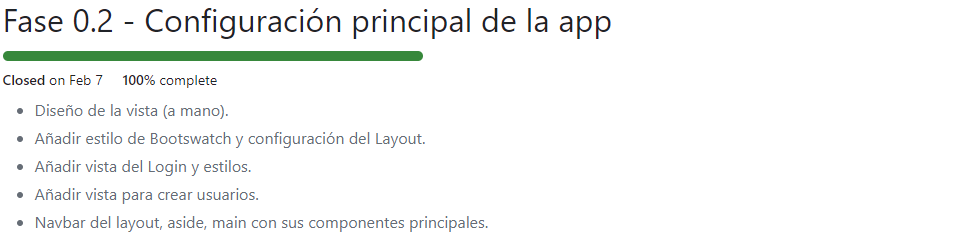
\includegraphics[width=\linewidth]{Fase0}
    \caption{Milestone de la fase 0}
\end{figure}
\newpage
La lista de las principales tareas que se han llevado a cabo en esta sección son:
\begin{itemize}
\tightlist
\item Diseño de las vistas principales.
\item Creación de las clases para los modelos de la base de datos.
\item Añadir el estilo principal de la aplicación.
\item Crear la vista del inicio de sesión (base).
\item Crear la vista para registrar usuarios (base).
\item Creación del layout principal con sus elementos.
\end{itemize}

El diseño inicial que se ha cogido como base para la aplicación se ha obtenido de 
\href{https://bootswatch.com/}{Bootswatch}\footnote{Bootswatch: https://bootswatch.com/}. Esta página tiene diseños gratuitos de
Bootstrap para su uso en cualquier aplicación web.

El diseño que se ha utilizado ha sido \href{https://bootswatch.com/flatly/}{\emph{Flatly}}\footnote{Diseño Flatly: https://bootswatch.com/flatly/}.

Para esta segunda parte, la duración estimada ha sido de 5 horas, y la duración real ha sido de 5 horas.

Al final, el total de tiempo estimado en esta fase cero ha sido de 8 horas, y el resultado
final ha sido de una duración de 8 horas y media, debido a diversos problemas con las versiones
de las dependencias, que ha alargado más la primera parte.

\subsection{Fase 1: \emph{Layout}, \emph{login}, registros y perfiles de los usuarios}
En esta fase, después de haber organizado la parte inicial de la aplicación, se comienza a llevar
a cabo el desarrollo principal del proyecto. 

Esta parte, en específico, comprende la gestión básica de los usuarios, creando la pantalla principal, el perfil, el registro de usuarios y el inicio de sesión correcto de los usuarios registrados.

Al igual que en el caso anterior, esta fase se divide en varias secciones:
\begin{itemize}
\tightlist
\item Fase 1.1: Configuración total del layout.
\item Fase 1.2: Inicio de sesión y registro de usuarios.
\item Fase 1.3: Configuración del perfil de los usuarios.
\end{itemize}

En la primera sección tenemos la configuración del layout. En esta parte se realizarán todas las
redirecciones a las diferentes vistas a las que se podrán acceder a través de este, el navbar
y la paginación de la pantalla principal.
\begin{figure}
    \centering
    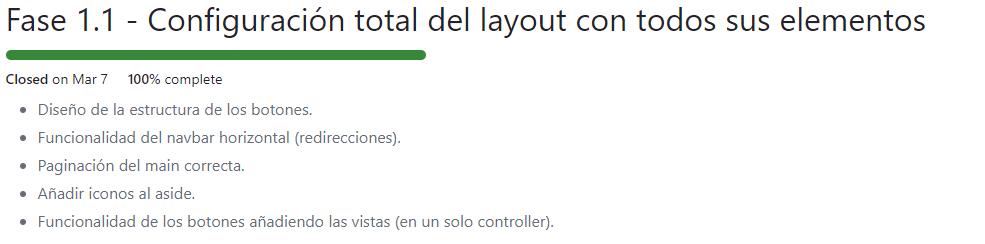
\includegraphics[width=\linewidth]{Fase1-1}
    \caption{Milestone de la fase 1.1}
\end{figure}

De esta forma, las tareas que se realizan son:
\begin{itemize}
\tightlist
\item Redirecciones al resto de vistas.
\item Añadir botones funcionales con el aside lateral.
\item Paginación de la pantalla principal.
\item Añadir iconos a las diferentes funciones.
\end{itemize}

Para esta primera parte, la duración prevista fue de una hora, y el tiempo real ha sido de una 
hora y media, debido a que la paginación del main se ha realizado a medida.

En la segunda sección se llevará a cabo el inicio de sesión y el registro de nuevos usuarios.
\begin{figure}
    \centering
    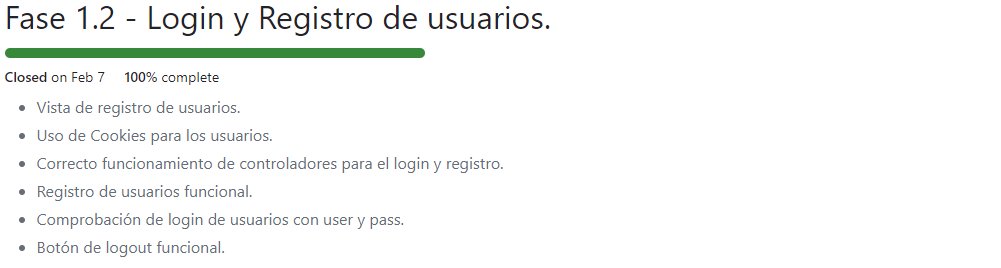
\includegraphics[width=\linewidth]{Fase1-2}
    \caption{Milestone de la fase 1.2}
\end{figure}
\newpage

La división de las tareas ha sido la siguiente:
\begin{itemize}
\tightlist
\item Vista del registro de usuarios completa y funcional.
\item Uso de ``cookies'' y variables de sesión para los usuarios.
\item Controladores para el inicio de sesión y registro.
\item Registro funcional de usuarios.
\item Comprobación de la funcionalidad del inicio de sesión.
\item Vista del inicio de sesión finalizada.
\item Logout de usuarios y limpieza de las \emph{cookies}.
\end{itemize}

Para las cookies he utilizado una dependencia que crea un objeto del modelo de base de datos.
En este objeto se puede añadir los atributos que se requieran, y se devuelve a la vista
para la permanencia de los datos. Gracias a este objeto, se pueden rellenar de datos las
variables de sesión para poder acceder a ellos en cualquier momento desde el controlador.

El tiempo estimado para estas tareas ha sido de 8 horas, y la duración final ha sido de 7 horas.

Por último, la tercera sección de esta fase comprende la configuración del perfil 
de los usuarios, y las tareas que se han llevado a cabo son:
\begin{itemize}
\tightlist
\item Vista para el perfil de los usuarios.
\item Creación de un modelo para guardar los datos principales.
\item Cambio de biografía y foto de perfil del usuario.
\item Cambio de la contraseña del usuario.
\end{itemize}

\begin{figure}
    \centering
    
\includegraphics[width=\linewidth]{Fase1-3}
    \caption{Milestone de la fase 1.3}
\end{figure}
Para esta sección se había considerado una duración de 5 horas, pero debido a la dificultad del
guardado de la foto de perfil en el servidor, se ha realizado en 6 horas.

La duración real total de esta fase ha sido de 14 horas y media.

\subsection{Fase 2: Directorio de usuario y gestión de currículos}
Esta fase comienza con la gestión de currículos desde el punto de vista del usuario, y se divide
en dos vistas: la vista del directorio y la vista de los currículos.

Como es una aplicación orientada al usuario, el directorio ofrece una gestión de archivos para este,
aunque por ahora solo se implementa un gestor de notas cortas.

Esta fase también tiene dos divisiones:
\begin{itemize}
\tightlist
\item Fase 2.1: Directorio del usuario y notas.
\item Fase 2.2: Comienzo con la gestión del currículum.
\end{itemize}

La primera parte tiene como objetivo crear la vista del directorio y hacer la funcionalidad
de las notas de los usuarios, de forma que tenemos las siguientes tareas:
\begin{itemize}
\tightlist
\item Vista para el directorio de los usuarios.
\item Botón para añadir nuevas notas.
\item Visualización de todas las notas del usuario en sesión.
\item Editar, borrar y ver el contenido de las notas.
\end{itemize}

\begin{figure}
    \centering
    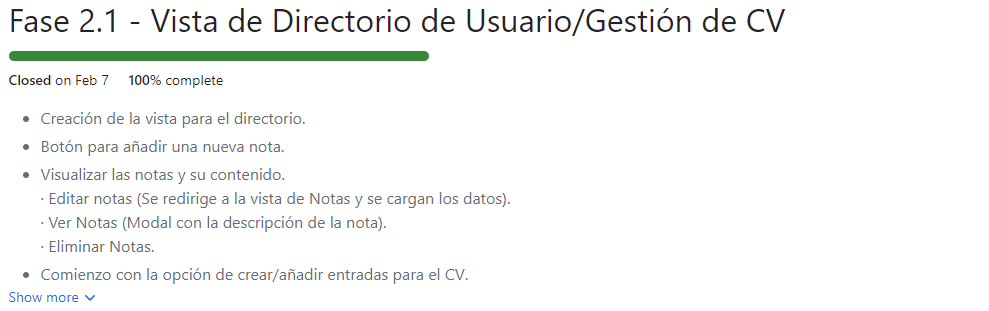
\includegraphics[width=\linewidth]{Fase2-1}
    \caption{Milestone de la fase 2.1}
\end{figure}

La duración de esta sección se ha estimado en 5 horas, que es lo que se ha invertido al final.

La segunda parte inicia la gestión de los currículos, y las tareas asignadas han sido:
\begin{itemize}
\tightlist
\item Creación de la vista para visualizar los currículos.
\item Botón para añadir un nuevo currículum.
\item Tabla con los iconos necesarios para los currículos.
\end{itemize}

\begin{figure}
    \centering
    
\includegraphics[width=\linewidth]{Fase2-2}
    \caption{Milestone de la fase 2.2}
\end{figure}

Para esta parte se han calculado 4 horas y se ha realizado en 3 horas. En total, el tiempo
estimado en esta fase ha sido de 9 horas y el tiempo invertido total ha sido de 8 horas, reduciendo
así el tiempo estimado en una hora.

\subsection{Fase 3: Edición, borrado, clonación y exportación de currículos}
Esta es la etapa más larga y en la que más tiempo se ha invertido en total, ya que es el 
núcleo o funcionalidad principal de la aplicación, que es la gestión de currículos.

Esta etapa se divide en varias secciones, igual que las anteriores:
\begin{itemize}
\tightlist
\item Fase 3.1: Edición de currículos.
\item Fase 3.2: Borrado de currículos.
\item Fase 3.3: Clonación de currículos.
\item Fase 3.4: Exportación a PDF.
\end{itemize}

La primera sección es el desarrollo principal de la gestión. Una vez se crea un currículum
y a parece en la tabla de la vista de los currículos, al dar al icono de editar se nos
abrirá una vista con las diferentes partes que comprenden un currículum para llenarlo de 
información. 

Toda la información del currículum se divide en un acordeón de html que tiene varios desplegables:
\begin{itemize}
\tightlist
\item 1: Información principal del usuario (nombre y apellidos, email, número, profesión...).
\item 2: Información académica.
\item 3: Idiomas.
\item 4: Experiencia laboral.
\item 5: Aptitudes y logros.
\end{itemize}

\begin{figure}
    \centering
    
\includegraphics[width=\linewidth]{Fase3-1}
    \caption{Milestone de la fase 3.1}
\end{figure}

Todas estas partes se pueden rellenar y guardar por igual, no son pasos sucesivos sino que están 
en la misma vista, para facilitar el guardado de los datos. Cada cambio en esta pantalla modifica
los datos del currículum.

Las tareas asignadas han sido:
\begin{itemize}
\tightlist
\item Creación de la vista con el acordeón.
\item Acordeón con las diferentes pasos de información al completo.
\item Guardado de todos los datos.
\end{itemize}

Todo lo que comprende esta vista, al ser demasiado grande, se ha valorado en unas 30 horas 
de trabajo, ya que en muchos casos la información es dinámica (pueden haber varias entradas
para idiomas, experiencia laboral y formación académica), de modo que se ha tenido que 
controlar el poder añadir varias entradas con JavaScript.

El tiempo total invertido ha sido de 33 horas finalmente.

La segunda parte se centra en el borrado de currículos existentes. A través de la tabla de
los currículos, hay un icono de una papelera con el que podremos borrar en su totalidad un
currículum.

Al hacer click sobre este botón, se nos mostrará un modal para confirmar la operación, y, al aceptar, el currículum se elimina de la base de datos y desaparece.

\begin{figure}
    \centering
    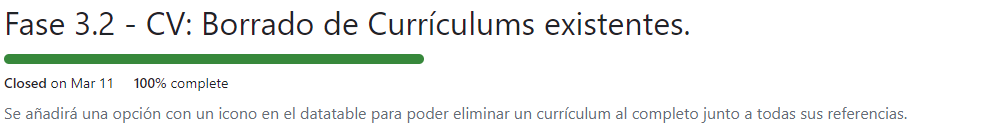
\includegraphics[width=\linewidth]{Fase3-2}
    \caption{Milestone de la fase 3.2}
\end{figure}

Como ha sido una sección corta, las tareas han sido la creación del modal para aceptar y la
funcionalidad del botón, por lo que se ha calculado una duración de 2 horas, y el tiempo real
invertido ha sido de finalmente 3 horas.

En tercer lugar, tenemos la clonación de currículos. Esta utilidad permite, desde la tabla
de los currículos, la posibilidad de copiar un currículum y crear uno idéntico, con los mismos 
datos. 

Esta funcionalidad se propuso para agilizar la creación de currículos similares y que contengan
al final los mismos datos.

\begin{figure}
    \centering
    
\includegraphics[width=\linewidth]{Fase3-3}
    \caption{Milestone de la fase 3.3}
\end{figure}

El tiempo estimado para la clonación fue de 4 horas y se realizó en 6 horas, debido a 
que había cierta dificultad para clonar las fotos del usuario.


Para finalizar con esta fase tenemos la exportación a PDF de los currículos. Se ha utilizado la
librería de Rotativa PDF, que permite exportar un objeto PDF desde el controlador, creando
a través de los datos del modelo y con una vista como plantilla, un documento en formato
PDF de los datos que se deseen.

Las tareas necesarias en esta fase han sido:
\begin{itemize}
\tightlist
\item Creación de la vista de la plantilla del pdf.
\item Llenar de datos el modelo que se va a utilizar.
\item Configuración de la librería y añadir los archivos principales.
\item Creación del objeto de Rotativa y hacer la exportación.
\end{itemize}

\begin{figure}
    \centering
    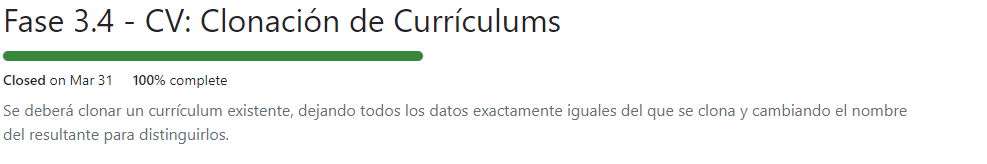
\includegraphics[width=\linewidth]{Fase3-4}
    \caption{Milestone de la fase 3.4}
\end{figure}

Además, para hacer la exportación se ha tenido en cuenta un formato específico, que es el
formato europeo de currículos. Este formato es el genérico utilizado en toda Europa en 
cuanto a empresas y administraciones públicas se refiere.

Para la realización de esta fase se han estimado 12 horas, y la duración final ha sido de 13 horas.

En el total de toda esta gestión de currículos, la duración prevista ha sido de 50 horas y el
tiempo total invertido ha sido de 55 horas.

\subsection{Fase 4: Gestión de currículos para administradores}
Esta fase no ha sido dividida en varias secciones debido a que se hace todo a través de la
misma pantalla.



Las diferencias entre las pantallas de los usuarios administradores y los normales son:
\begin{itemize}
\tightlist
\item El usuario no administrador solo puede ver sus currículos (y realizar el resto
de operaciones sobre su propio currículum).
\item El usuario administrador tiene un listado de todos los currículos que existen
en la base de datos y puede exportarlos a PDF o ver sus datos principales desde la
propia vista.
\item El usuario administrador, además, tiene varios campos por los que puede filtrar
los currículos para hacer una búsqueda más específica, si se requieren documentos
que cumplan ciertos requisitos (de idioma, rango de edad, etc.).
\end{itemize}

En esta fase, las tareas realizadas han sido las siguientes:
\begin{itemize}
\tightlist
\item Creación de la vista para la gestión de los currículos.
\item Listado de todos los documentos en una tabla con sus funcionalidades de ver y exportar.
\item Filtros para las búsquedas a través de varios de los campos.
\item Redirecciones y restricciones entre usuarios normales y administradores.
\item Funcionalidad de los filtros y los botones de ver y exportar.
\end{itemize}

\begin{figure}
    \centering
    
\includegraphics[width=\linewidth]{Fase4}
    \caption{Milestone de la fase 4}
\end{figure}

Para esta fase, se ha hecho una previsión de 18 horas, y la duración final de esta etapa ha sido
de 20 horas.

\subsection{Fase 5: Publicaciones en la página principal}
La página principal es la primera vista que vemos nada más iniciamos sesión en la aplicación.
En esta página se encuentras las publicaciones, que tienen un formato de red social y que 
funcionan como anuncios que pueden aportar información al usuario.

Junto a las publicaciones se implementan unos filtros de búsqueda, de forma similar a los
que hay en la gestión de currículos de los administradores.

Las tareas realizadas en esta fase han sido:
\begin{itemize}
\tightlist
\item Creación de la vista para las publicaciones.
\item Estructura de las publicaciones.
\item Filtros para la búsqueda de publicaciones.
\item Opción para añadir una publicación.
\end{itemize}

\begin{figure}
    \centering
    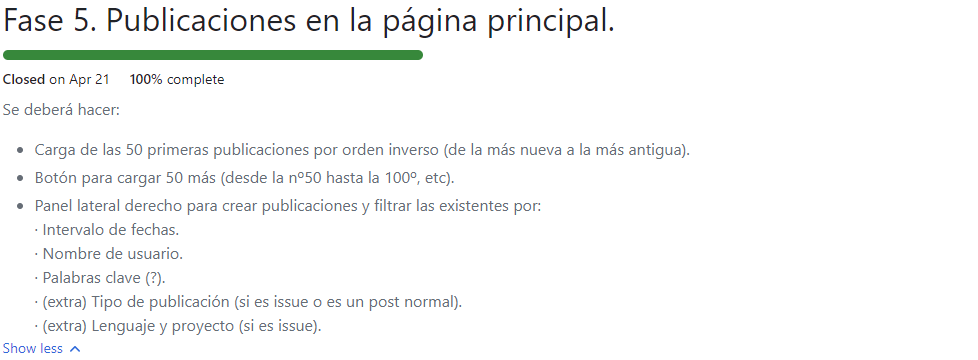
\includegraphics[width=\linewidth]{Fase5}
    \caption{Milestone de la fase 5}
\end{figure}

El tiempo estimado para la realización de estas tareas ha sido de 6 horas, completándolo todo
en un tiempo final de 6 horas.

\subsection{Fase 6: Administración y mantenimiento de usuarios}
El mantenimiento de usuarios es muy similar a la vista de gestión de currículos de los
administradores. 

Por un lado tenemos una lista de todos los usuarios en una tabla y por
otro podemos cargar y visualizar los datos de los usuarios para cambiarlos.

Las tareas realizadas en esta fase han sido:
\begin{itemize}
\tightlist
\item Creación de la vista para el mantenimiento de usuarios.
\item Tabla con los usuarios.
\item Visualización de los datos de los usuarios a través de un botón.
\item Edición de los datos de los usuarios.
\end{itemize}

\begin{figure}
    \centering
    
\includegraphics[width=\linewidth]{Fase6}
    \caption{Milestone de la fase 6}
\end{figure}

La duración prevista para el desarollo de esta fase ha sido de 7 horas y se ha completado en 8
horas, aumentando así el tiempo estimado en una hora.

\subsection{Fase 7: Despliegue de la aplicación en servidor con una máquina virtual}
El despliegue de la aplicación es la más importante para las pruebas y la solución
final. Como se ha explicado previamente, el servidor web se creará a través de una
máquina virtual de Windows 10, que genera un servidor local a través del IIS Express.

El proceso de construcción del servidor tiene los siguientes pasos o tareas:
\begin{itemize}
\tightlist
\item 1. Se crea la máquina virtual de Windows 10.
\item 2. Se instancian el SQL Server y el SQL Management Studio y se añade la base de datos.
\item 3. Se configura el IIS que genera la instancia del servidor de la web.
\item 4. Se publica la aplicación en un directorio y se apunta a este desde el IIS.
\item 5. Se genera una dirección local para acceder a ella desde un navegador.
\end{itemize}
La máquina virtual se exportará como un archivo en formato ``.ova'' que se importará
directamente a VirtualBox o VMWare (en función de la aplicación que se use para 
gestionar las máquinas virtuales).

\begin{figure}
    \centering
    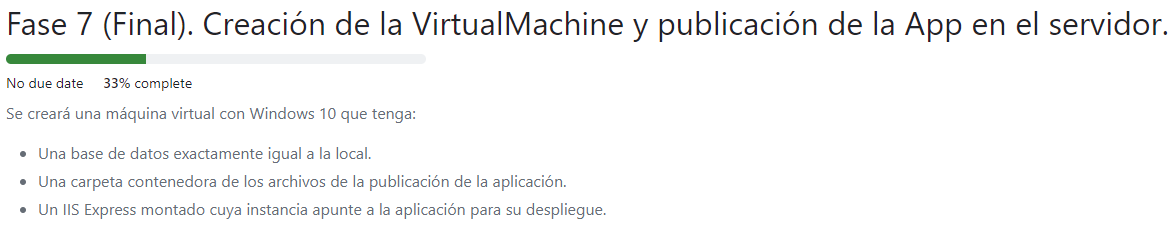
\includegraphics[width=\linewidth]{Fase7}
    \caption{Milestone de la fase 7}
\end{figure}

La máquina virtual tiene ciertas necesidades a la hora de instalarla, por lo tanto dependerá 
del equipo en el que lo instalemos. Debido a esto, hay que comprobar que el sistema anfitrión cumpla unos requerimientos de memoria, procesadores, etc.

Para ello, se aportan los datos de la máquina virtual, que son los siguientes:
\begin{table}[h]
	\centering
	\begin{tabular}{lc }
		\toprule
		\textbf{Característica}    & \textbf{Valor}\\
		\toprule
  	\text{Sistema Operativo}                & Windows 10 Home    \\
		\text{Memoria Virtual}                  & 50 GB   \\
		\text{Memoria RAM}                      & 4 GB \\
		\text{Procesadores}                     & 3-4 procesadores\\
		\bottomrule
	\end{tabular}
	\caption{Datos Máquina Virtual}
\end{table}

Para crear la máquina virtual y configurar todo lo necesario ha sido necesario invertir 20 horas de trabajo.


\subsection{Fase 8: Mejoras y extras}
La fase de mejoras es un añadido que está fuera del alcance del proyecto (esto se explicará
más adelante). En esta etapa se han añadido las tareas que, o bien eran las menos prioritarias,
o bien estaban estimadas como mejoras a la aplicación una vez estuviera terminada.

En esta fase podemos ver tareas como las siguientes:
\begin{itemize}
\tightlist
\item Mejoras y cambios en el diseño general de la aplicación.
\item Añadir el registro de usuarios en el inicio de sesión.
\item Añadir campo booleano activo a varias tablas para su mantenimiento.
\item Añadir contactos dentro de la aplicación.
\item Respuestas a publicaciones y notificaciones.
\item Añadir campos y atributos nuevos a los currículos.
\item Filtros nuevos en la gestión de usuarios y currículos para los administradores.
\end{itemize}

\begin{figure}
    \centering
    
\includegraphics[width=\linewidth]{Fase8}
    \caption{Milestone de la fase 8}
\end{figure}

Como las mejoras están fuera del alcance del proyecto, no se estima una duración exacta,
ya que son tareas que se proponen a futuro y debido a que forman una lista que puede
alargarse con más procesos. La duración total ha sido de 35 horas, contando la revisión y corrección de errores.

\subsection{Fase 9: Documentación}
La documentación es la última parte del desarrollo de este proyecto, pero es algo que se ha ido haciendo de manera progresiva a lo largo de este. En esta fase se incluye la documentación de los siguientes apartados:
\begin{itemize}
\tightlist
\item Anexos (este documento).
\item Memoria.
\item Manuales de instalación, del programador y de usuario.
\item Casos de uso.
\item Diagramas E/R de los modelos.
\end{itemize}

Todos los materiales que se han querido documentar están tanto en la memoria como en 
los anexos. Al principio se quería incluir los casos de uso y los manuales en archivos
por separado, pero al final se han acabado incluyendo en los anexos.

En la documentación tenemos las siguientes tareas:
\begin{itemize}
\tightlist
\item Búsqueda de información bibliográfica y preparación de los documentos.
\item Obtención de imágenes, tablas y figuras que aportan información.
\item Formato y estructura de la memoria y anexos correctos.
\item Documentar todos los puntos de la estructura de la memoria y de los anexos.
\item Tablas para los casos de uso.
\item Compilación de imágenes de ejemplo para los manuales de instalación y usuario.
\item Revisión de errores y avisos con el editor de Overleaf antes de la entrega.
\end{itemize}

La duración valorada para la memoria ha sido la más larga de todas las fases, siendo esta de
45-48 horas. 

En la tabla \ref{duracionDoc} se muestra la duración total de cada una de las partes de la documentación.
\begin{table}
	\centering
	\begin{tabular}{ lr }
		\toprule
		\textbf{Documentación}    & \textbf{Horas invertidas}\\
		\toprule
		\text{Memoria}                          & 25 h  \\
		\text{Anexos (A-D)}                     & 40 h \\
		\text{Manuales}                         & 20 h \\
		\text{Casos de uso}                     & 20 h \\
        \text{Imágenes y figuras}               & 5 h \\
		\text{Investigación}                    & 15 h \\
		\text{Revisión y corrección}            & 5 h \\
		\bottomrule
		\textbf{Total horas invertidas}    & 130 h\\
	\end{tabular}
	\caption{Duración total de la documentación}
    \label{duracionDoc}
\end{table}


\begin{table}
	\centering
	\begin{tabular}{lr}
		\toprule
		\textbf{Fase}    & \textbf{Horas invertidas}\\
		\toprule
		\text{Fase 1: Análisis y configuraciones}         & 30 h  \\
		\text{Fase 2: Directorio de usuarios}             & 8 h \\
		\text{Fase 3: Edición de currículos}                    & 55 h \\
		\text{Fase 4: Administración de currículos}             & 20 h \\
        \text{Fase 5: Publicaciones en index}             & 6 h \\
        \text{Fase 6: Administración de usuarios}         & 8 h \\
        \text{Fase 7: Despliegue servidor}                & 20 h \\
        \text{Fase 8: Mejoras, extras y revisión}         & 35 h \\
        \text{Fase 9: Documentación}                      & 130 h \\
		\bottomrule
		\textbf{Total horas invertidas}    & 312 h\\
	\end{tabular}
	\caption{Horas invertidas totales de las fases}
    \label{duracionTot}
\end{table}
Finalmente, la duración total de todas las fases se muestra en la tabla \ref{duracionTot}.

\newpage
\section{Estudio de viabilidad}
\subsection{Viabilidad económica}
La aplicación se desarrolla en un entorno y marco de trabajo de código abierto, ya que se utilizan herramientas software como SQL Management Studio y Visual Studio Community 2022 para su desarrollo, herramientas que ofrece Microsoft de forma gratuita.

Además para el despliegue de la web se utilizará una máquina virtual con Windows 10 de forma local, por lo que no hará falta alojarla en un servidor de pago, solo en el contexto de la empresa se deberá contemplar este último punto, para añadir el proyecto como una nueva instancia al servidor de esta junto al resto de aplicaciones internas.

Debido a este último punto, se hará un análisis realista de los gastos económicos que supondrían
para una empresa, divididos en varios tipos de costes:
\begin{itemize}
\tightlist
\item Costes de personal.
\item Costes de material y derivados de la empresa.
\end{itemize}

Se va a suponer que la duración del proyecto han sido las 300 horas que se recogen en la 
guía docente del TFG a la que incluimos 60 horas de planificación en la empresa, instalación
y pruebas, de manera que distribuido equitativamente en jornadas laborales de 8 horas al día durante 5 días a la semana, tenemos:

360 horas / (8 horas * jornada) = 40 jornadas

Tenemos 40 jornadas, que con 5 a la semana son aproximadamente dos meses de trabajo.

\subsubsection{Coste de personal}
El coste del personal equivaldrá al salario de la persona que realice el proyecto. En 
este caso vamos a considerar que solo tenemos un trabajador y que se considera la nómina de la tabla \ref{tablaNomina}.

\begin{table}
	\centering
	\begin{tabular}{lr }
		\toprule
		\textbf{Conceptos}    & \textbf{Costes}\\
		\toprule
		\text{Salario Base}                     & 950€   \\
		\text{Convenios}                        & 250€ \\
		\text{Complementos}                     & 250€ \\
		\text{Total devengo (bruto)}            & 1450€ \\
		\text{Retenciones (IRPF 15\% y otros)}  & 250€ \\
		\text{Seguridad Social (28,3\%)}        & 406€ \\
		\bottomrule
		\textbf{Total en dos meses}    & 3712€\\
	\end{tabular}
	\caption{Coste de personal}
    \label{tablaNomina}
\end{table}

\subsubsection{Coste de material y general de la empresa}
En cuanto al material necesario para la realización del proyecto, tenemos, por un lado, el 
equipo o el dispositivo en el que se realizará (hardware) y, por otro lado, el software
necesario que tendrá este equipo. 

Por otro lado debemos analizar los gastos internos de la empresa, tales como alquiler de oficinas
y su mantenimiento (luz, agua, Internet, etc.), servidores y otras licencias.

De esta forma, podemos observar el costo total en la tabla \ref{tablaCostosEmpresa}.

\begin{table}
	\centering
	\begin{tabular}{lr }
		\toprule
		\textbf{Conceptos}    & \textbf{Costes}\\
		\toprule
		\text{Portátil}                         & 900€   \\
		\text{Windows 10 Home}                  & 145€ \\
        \text{Servidor (mes)}                   & 125€ \\
        \text{Oficina + mantenimientos (mes)}   & 1000€ \\
        \text{Internet}                         & 180-200€ \\
        \text{Dominio de GitLab Ultimate (mes)} & 100€ \\
		\bottomrule
		\textbf{Total}    & 2450-2470€\\
	\end{tabular}
	\caption{Coste material y general de la empresa}
    \label{tablaCostosEmpresa}
\end{table}

\subsection{Viabilidad legal}
En esta segunda parte de la viabilidad, se describirán las licencias de las herramientas 
software utilizadas y de la documentación del proyecto.

Las herramientas, librerías y dependencias que se utilizan están sujetas a licencias. Una 
licencia es la forma en la que se distribuye el uso de un proyecto, una copia de este o su
documentación.

Incluso aunque una herramienta sea de código abierto, este está sujeto a una licencia que permite
que, de forma legal, el producto pueda ser utilizado de forma libre.

De esta forma se profundizará en las herramientas utilizadas y qué tipo de viabilidad 
legal tienen. Podemos dividirlo en dos secciones: por un lado tenemos las herramientas
con las que viene Visual Studio, o también llamadas herramientas internas. Por otro lado, las
herramientas externas, pueden ser, por ejemplo, \emph{Bootstrap}, \emph{Rotativa}, \emph{Datatables}, etc.

\subsubsection{Licencias Internas}
Como se ha mencionado previamente, las licencias internas serán:
\begin{itemize}
\tightlist
\item Dependencias del proyecto.
\item Librerías y paquetes NuGet.
\item Visual Studio.
\item Windows 10 Home.
\item SQL Management Studio.
\end{itemize}

Todas las licencias de las herramientas mencionadas forman parte de ``Microsoft Corporation'', ya
que son herramientas proporcionadas por Microsoft. Todas las anteriores, menos Windows 10, son
de uso libre.

Para crear la máquina virtual, el Windows 10 que se utiliza se crea a mano gracias a un 
archivo ``.iso'' que se genera gracias a una herramienta gratuita de Microsoft. Como no tiene
licencia, está sujeta a las mismas condiciones que Windows 10.

\subsubsection{Licencias Externas}
En cuanto a las licencias externas, tenemos:
\begin{itemize}
\tightlist
\item \emph{Bootstrap} y \emph{Bootswatch}.
\item \emph{Fontawesome}.
\item \emph{RotativaPDF}.
\item \emph{Datatables}.
\item \emph{JQuery}.
\end{itemize}

Las licencias de las librerías anteriores se muestran en la tabla \ref{tablaLicencias}.
\begin{table}
	\centering
	\begin{tabular}{lc}
		\toprule
		\textbf{Librería}    & \textbf{Licencia}\\
		\toprule
		\text{Bootstrap y Bootswatch}           & MIT license   \\
		\text{Fontawesome Fonts}                & SIL OFL 1.1 \\
  	\text{Fontawesome Code}                 & MIT license \\
    	\text{Fontawesome Documentation}        & CC BY 3.0 \\
        \text{JQuery}                           & MIT license \\
        \text{RotativaPDF}                      & MIT license \\
        \text{Datatables}                       & MIT license \\
		\bottomrule
	\end{tabular}
	\caption{Licencias de las librerías externas}
    \label{tablaLicencias}
\end{table}

\section{Licencias propias}
Hemos hablado de los diferentes tipos de licencias que se encuentran en las librerías y dependencias que se utilizan en el proyecto. En este apartado, veremos las licencias que tiene el proyecto en sí.

En el contexto de este proyecto, se van a dividir las licencias en función de cada una de las partes que componen este. Principalmente se usará la licencia de atribución, aunque se diferenciará su alcance entre código y documentación, teniendo como resultado el resumen de la tabla \ref{licenciasProyecto}.

Como el código que se desarrolla forma parte del desarrollo de un proyecto real de una empresa, se añade la particularidad de que sea no comercial, no siendo este el caso para el resto de los adjuntos de este proyecto.
\begin{table}
	\centering
	\begin{tabular}{lc }
		\toprule
		\textbf{Librería}    & \textbf{Licencia}\\
		\toprule
		\text{Código Interno}                   & CC BY-NC 4.0   \\
		\text{Máquina Virtual}                  & CC BY 4.0 \\
  	\text{Imágenes}                         & CC BY 4.0 \\
    	\text{Repositorio}                      & CC BY 4.0 \\
        \text{Documentación}                    & CC BY 4.0 \\
		\bottomrule
	\end{tabular}
	\caption{Licencias del proyecto}
    \label{licenciasProyecto}
\end{table}
\apendice{Especificación de Requisitos}
\section{Introducción}
En esta sección se detallarán los diferentes requisitos de la aplicación en base a los objetivos principales de esta, diviendo en varios tipos de requisitos para su posterior desarrollo.

En primer lugar, es necesario observar cuáles son los requisitos de la aplicación, qué
se quiere conseguir y cómo se hará. Esto sirve de base de análisis por el equipo a la
hora de gestionar las distintas fases del desarrollo de la aplicación.

Como los requisitos dependen de los objetivos iniciales de la aplicación, deben cumplir una serie
de características:
\begin{itemize}
 \item Debe haber claridad a la hora de su especificación.
 \item Se organizan en función de una metodología y se deben priorizar ciertos objetivos.
 \item Se debe probar el éxito o fracaso de la aplicación en tiempo finito.
 \item Se debe ser coherente a la hora de estimar los tiempos para lograr los
 objetivos que estiman dentro del alcance del proyecto.
 \item Se deben tener en cuenta todos los objetivos que se proponen.
\end{itemize}

\section{Objetivos Generales}
El objetivo principal del desarrollo de la aplicación es proporcionar un entorno web con un formato de red social dedicado al usuario, que permita:
\begin{itemize}
 \item Una gestión básica de usuarios (perfiles, notas, configuración).
 \item Gestión de currículos de los usuarios de la empresa.
 \item Gestión de directorios y notas de los usuarios.
 \item Gestión de currículos y usuarios por parte de los usuarios administradores de la empresa.
 \item Facilidad para buscar y filtrar información de usuarios y currículos.
 \item Sencillez y comodidad en la interacción entre el usuario y la aplicación.
 \item Ofrecer más funcionalidades a futuro, mantenimiento y actualizaciones en nuevas fases.
 \item Accesibilidad y estructura correcta de los datos que se manejan.
\end{itemize}

\section{Catálogo de requisitos}
Los requisitos se van a dividir en tres secciones:
\begin{itemize}
\tightlist
 \item \textbf{Requisitos Estructurales}: se describe la estructura de la aplicación.
 \item \textbf{Requisitos Funcionales}: requisitos del funcionamiento y comportamiento
 de la aplicación. En este apartado se enumeran los casos de uso, pero estos se tratarán en un
 apartado específico.
 \item \textbf{Requisitos No Funcionales}: requisitos impuestos a un sistema para la calidad
 y mantenimiento del software.
\end{itemize}

\subsection{Requisitos estructurales}
Los requisitos estructurales son la base de la aplicación. En este apartado se incluirán:
\begin{itemize}
\tightlist
 \item Base de Datos: tablas necesarias para el desarrollo de la aplicación y el guardado de los datos.
 \item Vistas necesarias para la funcionalidad de la aplicación que cumplan los objetivos definidos previamente.
 \item Despliegue de la web.
\end{itemize}

\subsubsection{Base de Datos}
La base de datos se instanciará en local y accederemos a través de SQL Management Studio 18. Las entidades o tablas requeridas para los objetivos marcados son:
\begin{itemize}
 \item Usuario: tabla para los usuarios.
 \item Currículum: tabla que guarda la instancia de un currículum. Es la tabla madre de la gestión de currículos, y de ella heredarán otras como FormacionCV, EntradaCV, UsuarioCV (es decir, todas las distintas fases que comprenden el currículum al completo), etc.
 \item Entrada: una tabla para guardar las publicaciones de los usuarios.
 \item NotaUsuario: tabla dedicada a guardar las notas personales de los usuarios.
\end{itemize}

\subsubsection{Vistas de la aplicación}
Al ser una aplicación web, las vistas forman el nexo entre la interacción del usuario con esta. Para cumplir los objetivos que se han definido anteriormente, serán necesarias las siguientes vistas o pantallas:
\begin{itemize}
 \item \textbf{\emph{Login} o inicio de sesión}: primera pantalla, para iniciar sesión en la aplicación con el usuario.
 \item \textbf{\emph{Layout} o disposición de la página}: vista que formará la interfaz de la aplicación (es la madre del resto de vistas, aparecerá en todo momento como una capa externa). En esta se dotará de un navegador superior y un panel lateral con las distintas opciones de navegación (para la gestión de currículos, perfil, etc.).
 \item \textbf{Gestor de currículos}: una vista principal donde se muestren los currículos del usuario conectado con opciones para editar, eleminar y exportar a PDF. Los administradores verán
 un listado de todos los currículos en base de datos y podrán filtrarlos a través
 de varios campos.
 \item \textbf{Gestor de usuarios}: los administradores tendrán una lista con los usuarios activos
 y podrán gestionarlos (editar datos, desactivarlos, asignar gestores, etc.).
 \item \textbf{Editor de perfil}: una vista con los datos de usuario que permita modificar/añadir distintos datos de información de usuario.
 \item \textbf{Notas}: una vista para que el usuario pueda crear, editar y eliminar notas personales.
 \item \textbf{Entradas}: la vista principal de la aplicación que será parte del inicio, que muestre las diferentes publicaciones de los usuarios y permita filtrar y añadir nuevas publicaciones.
\end{itemize}

\subsubsection{Despliegue de la web}
Una vez esté terminada la aplicación se deberá desplegar para poder utilizarla. Depende del contexto del proyecto, el despliegue de este se dividirá en dos formas.

Por un lado, el despliegue en local se hará a través de una máquina virtual con Windows 10, que tendrá una base de datos con SQL Management y un ejecutable de la aplicación. Esto se hará para poder ejecutar la aplicación de forma local, y se proporcionará la imagen del disco para su uso.

Por otro lado, en el contexto de la empresa, la aplicación se deberá alojar en el servidor SQL Server de esta, creando una instancia para la publicación web del proyecto y añadiendo la base de datos correspondiente.

\subsection{Requisitos funcionales de la aplicación}
Los requisitos funcionales de la aplicación comprenden el comportamiento de la aplicación
en cuanto a su funcionalidad, y se relaciona de forma directa con las distintas fases por las que pasará el proyecto. 

Para este tipo de requisitos se hará un conjunto de casos de uso, que son pruebas de funcionalidad
de las distintas fases o apartados que tiene la aplicación. Los requisitos funcionales
son los siguientes:
\begin{itemize}
\tightlist
 \item \textbf{RF-01}: Inicio de sesión en la aplicación.
 \item \textbf{RF-02}: Página principal.
    \begin{itemize}
    \tightlist
     \item \textbf{RF-02.1}: Crear publicaciones.
     \item \textbf{RF-02.2}: Filtrar publicaciones.
    \end{itemize}
 \item \textbf{RF-03}: Configuración del perfil de los usuarios.
 \item \textbf{RF-04}: Directorio de usuarios.
    \begin{itemize}
    \tightlist
     \item \textbf{RF-04.1}: Crear notas de usuario.
     \item \textbf{RF-04.2}: Ver y editar notas de usuario.
     \item \textbf{RF-04.3}: Borrar notas de usuario.
    \end{itemize}
 \item \textbf{RF-05}: Listar currículos.
    \begin{itemize}
    \tightlist
     \item \textbf{RF-05.1}: Crear currículos.
     \item \textbf{RF-05.2}: Editar currículos.
     \item \textbf{RF-05.3}: Borrar currículos.
     \item \textbf{RF-05.4}: Clonar currículos.
     \item \textbf{RF-05.5}: Exportación a PDF.
     \item \textbf{RF-05.6}: Filtrar currículos.
     \item \textbf{RF-05.7}: Ver datos de currículos.
    \end{itemize}
 \item \textbf{RF-06}: Listar usuarios.
    \begin{itemize}
    \tightlist
     \item \textbf{RF-06.1}: Modificar usuarios.
    \end{itemize}
 \item \textbf{RF-07}: Registrar usuarios.
\end{itemize}

Para los casos de uso tenemos dos tipos de actores: el usuario administrador y el usuario normal.
En función del usuario con el que iniciemos sesión, podremos acceder a unas funciones u otras.

De esta manera, podemos dividir los casos de uso con los diferentes actores en la tabla \ref{casosUsoResumen}.
\begin{table}
    \centering
	\begin{tabular}{lc}
		\toprule
		\textbf{Caso de uso}    & \textbf{Actor involucrado}\\
		\toprule
        \text CU-01: Inicio de sesión en la aplicación            & Ambos  \\
        \text CU-02: Página principal                             & Ambos  \\
        \text CU-03: Configuración del perfil de los usuarios     & Ambos  \\
        \text CU-04: Directorio de usuarios                       & Ambos  \\
        \text CU-05: Listar currículos                           & Ambos \\
        \text CU-06: Crear currículos                            & No administrador \\
        \text CU-07: Editar currículos                           & No administrador \\
        \text CU-08: Borrar currículos                           & No administrador \\
        \text CU-09: Clonar currículos                           & No administrador \\ 
        \text CU-10: Exportación a PDF                            & Ambos  \\
        \text CU-11: Filtrar currículos                          & Administrador \\
        \text CU-12: Ver datos de currículos                     & Administrador \\
        \text CU-13: Filtrar publicaciones                        & Ambos  \\
        \text CU-14: Crear publicaciones                          & Ambos  \\
        \text CU-15: Listar usuarios                              & Administrador \\
        \text CU-16: Modificar usuarios                           & Administrador \\
        \text CU-17: Crear notas de usuario                       & Ambos  \\
        \text CU-18: Ver y editar notas de usuario                & Ambos  \\
        \text CU-19: Borrar notas de usuario                      & Ambos  \\
        \text CU-20: Registrar usuarios                           & Administrador  \\
		\bottomrule
	\end{tabular}
	\caption{Tabla de Casos de Uso}
    \label{casosUsoResumen}
\end{table}


\subsection{Requisitos no funcionales de la aplicación}
Los requisitos no funcionales de un sistema son aquellas restricciones que definen los
aspectos de un sistema en cuanto a calidad, rendimiento y seguridad de este, entre otros.

Hay muchos tipos de requisitos no funcionales, pero se destacarán los siguientes:
\begin{itemize}
\item
  \textbf{Rendimiento:} para que una aplicación tenga buen rendimiento, en el caso
  de una página web, debe permitir el acceso y cambio entre vistas en el menor tiempo 
  posible, evitando consultas de datos muy grandes y tiempos de procesamiento elevados.
\item
  \textbf{Seguridad:} la aplicación debe estar protegida contra el acceso no autorizado. 
  En el caso de una aplicación web, debe haber una forma lógica y segura de la estructura
  de las claves en la base de datos, como por ejemplo el uso de claves encriptadas, hash, etc.
\item
  \textbf{Actuación:} la aplicación debe ser capaz de manejar una gran cantidad de datos
  y de usuarios sin poner en riesgo el rendimiento de esta.
\item
  \textbf{Disponibilidad:} la aplicación debe estar disponible de forma sencilla y 
  evitando problemas de acceso al sistema (Internet, acceso a la aplicación por dominio o dirección,
  etc.).
\item
  \textbf{Escalabilidad:} la aplicación será capaz de seguir ampliándose y desarrollándose
  a futuro sin bajar o degradar su rendimiento.
\item
  \textbf{Mantenimiento}: la aplicación debe ser fácil de mantenerse con el tiempo y favorecer
  la escalabilidad en cuanto a actualizaciones y cambios.
\item
  \textbf{Usabilidad}: la aplicación debe ser intuitva y fácil de utilizar. Un manual de usuario
  también facilita la usabilidad del sistema.
\item
  \textbf{Compatibilidad y portabilidad}: el sistema debe ser compatible con otras aplicaciones.
  En este caso se incluyen los diferentes navegadores web por los que se puede acceder 
  a la aplicación, o las migraciones de la base de datos y del propio programa con actualizaciones de estrucuturas internas como servidores, entornos, etc.
\item
  \textbf{Fiabilidad}: el sistema debe dotar de confianza al usuario y su uso debe cumplir
  con los objetivos y requerimientos que se buscan con la aplicación.
\end{itemize}

\newpage

\section{Casos de uso}
% Caso de Uso 01 -> Inicio de sesión en la aplicación.
\begin{table}[h]
	\centering
	\begin{tabularx}{\linewidth}{ p{0.21\columnwidth} p{0.7\columnwidth} }
		\toprule
		\textbf{CU-01}    & \textbf{Inicio de sesión en la aplicación}\\
		\toprule
		\text{Versión}              & 1.0    \\
		\text{Autor}                & Alex Tomé \\
        \text{Actores}              & Usuario genérico y administrador \\
		\text{R.F asociados}        & RF-01 \\
		\text{Descripción}          & Se debe entrar en la aplicación con usuario y contraseña \\
		\text{Precondición}         & Usuario registrado en el sistema con contraseña \\
		\text{Acciones}             &
		\begin{enumerate}
			\def\labelenumi{\arabic{enumi}.}
			\tightlist
			\item El usuario introduce nombre de usaurio y contraseña
			\item El usuario pulsa el botón de entrar.
		\end{enumerate}\\
		\text{Postcondición}        & El usuario entra con éxito al sistema \\
		\text{Excepciones}          & No existe el usuario o las credenciales son incorrectas \\
		\text{Importancia}          & Alta \\
		\bottomrule
	\end{tabularx}
	\caption{CU-1 Inicio de sesión en la aplicación.}
\end{table}


% Caso de Uso 02 -> Vista de publicaciones.
\begin{table}[H]
	\centering
	\begin{tabularx}{\linewidth}{ p{0.21\columnwidth} p{0.7\columnwidth} }
		\toprule
		\textbf{CU-02}    & \textbf{Vista de publicaciones}\\
		\toprule
		\text{Versión}              & 1.0    \\
		\text{Autor}                & Alex Tomé \\
        \text{Actores}              & Usuario genérico y administrador \\
		\text{R.F asociados}        & RF-02 \\
		\text{Descripción}          & Se podrán ver las publicaciones de la página principal \\
		\text{Precondición}         & Usuario con sesión en el sistema \\
		\text{Acciones}             &
		\begin{enumerate}
			\def\labelenumi{\arabic{enumi}.}
			\tightlist
			\item El usuario entra en la aplicación tras iniciar sesión.
            \item El usuario ve las últimas publicaciones.
		\end{enumerate}\\
		\text{Postcondición}        & El usuario ve las publicaciones con éxito \\
		\text{Excepciones}          & No cargan las publicaciones \\
		\text{Importancia}          & Media \\
		\bottomrule
	\end{tabularx}
	\caption{CU-02 Vista de publicaciones.}
\end{table}

% Caso de Uso 03 -> Configuración del perfil.
\begin{table}[H]
	\centering
	\begin{tabularx}{\linewidth}{ p{0.21\columnwidth} p{0.71\columnwidth} }
		\toprule
		\textbf{CU-03}    & \textbf{Configuración del perfil}\\
		\toprule
		\text{Versión}              & 1.0    \\
		\text{Autor}                & Alex Tomé \\
        \text{Actores}              & Usuario genérico y administrador \\
		\text{R.F asociados}        & RF-03 \\
		\text{Descripción}          & Se podrá acceder al perfil y editar datos \\
		\text{Precondición}         & Usuario con sesión en el sistema \\
		\text{Acciones}             &
		\begin{enumerate}
			\def\labelenumi{\arabic{enumi}.}
			\tightlist
			\item El usuario entra en su perfil.
            \item El usuario puede cambiar datos a placer.
            \item Los datos cabiados se guardan al pulsar el botón de guardar.
		\end{enumerate}\\
		\text{Postcondición}        & El usuario guarda los cambios con éxito  \\
		\text{Excepciones}          & El usuario no puede modificar los datos \\
		\text{Importancia}          & Alta \\
		\bottomrule
	\end{tabularx}
	\caption{CU-03 Configuración del perfil.}
\end{table}

% Caso de Uso 04 -> Directorio de usuarios.
\begin{table}[H]
	\centering
	\begin{tabularx}{\linewidth}{ p{0.21\columnwidth} p{0.71\columnwidth} }
		\toprule
		\textbf{CU-04}    & \textbf{Directorio de usuarios}\\
		\toprule
		\text{Versión}              & 1.0    \\
		\text{Autor}                & Alex Tomé \\
        \text{Actores}              & Usuario genérico y administrador \\
		\text{R.F asociados}        & RF-04, RF-04.1, RF-04.2 \\
		\text{Descripción}          & Se podrá acceder al directorio y ver las notas \\
		\text{Precondición}         & Usuario con sesión en el sistema \\
		\text{Acciones}             &
		\begin{enumerate}
			\def\labelenumi{\arabic{enumi}.}
			\tightlist
			\item El usuario entra en el directorio personal.
            \item El usuario ve un listado de las notas creadas y un botón para añadir nuevas.
		\end{enumerate}\\
		\text{Postcondición}        & El usuario ve las notas con éxito \\
		\text{Excepciones}          & No carga el directorio \\
		\text{Importancia}          & Media \\
		\bottomrule
	\end{tabularx}
	\caption{CU-04 Directorio de usuarios.}
\end{table}

% Caso de Uso 05 -> Listar currículos.
\begin{table}[H]
	\centering
	\begin{tabularx}{\linewidth}{ p{0.21\columnwidth} p{0.71\columnwidth} }
		\toprule
		\textbf{CU-05}    & \textbf{Listar currículos}\\
		\toprule
		\text{Versión}              & 1.0    \\
		\text{Autor}                & Alex Tomé \\
        \text{Actores}              & Usuario genérico y administrador \\
		\text{R.F asociados}        & RF-05, RF-05.1, RF-05.6, RF-05.7 \\
		\text{Descripción}          & Se podrá acceder y ver los documentos creados por el                                      usuario (usuario genérico). Se listarán los currículos de                                  todo el sistema (administrador) \\
		\text{Precondición}         & Usuario con sesión en el sistema \\
		\text{Acciones}             &
		\begin{enumerate}
			\def\labelenumi{\arabic{enumi}.}
			\tightlist
			\item El usuario entra en la vista de currículos.
            \item Si es administrador, verá un listado de todos los currículos. Si no lo es, verá solo los currículos creados por ese usuario.
		\end{enumerate}\\
		\text{Postcondición}        & El usuario ve los currículos  \\
		\text{Excepciones}          & El usuario no puede ver el listado \\
		\text{Importancia}          & Alta \\
		\bottomrule
	\end{tabularx}
	\caption{CU-05 Listar currículos.}
\end{table}

% Caso de Uso 06 -> Crear currículos.
\begin{table}[H]
	\centering
	\begin{tabularx}{\linewidth}{ p{0.21\columnwidth} p{0.71\columnwidth} }
		\toprule
		\textbf{CU-06}    & \textbf{Crear currículos}\\
		\toprule
		\text{Versión}              & 1.0    \\
		\text{Autor}                & Alex Tomé \\
        \text{Actores}              & Usuario genérico \\
		\text{R.F asociados}        & RF-05, RF-05.1 \\
		\text{Descripción}          & Se podrá crear un nuevo currículum \\
		\text{Precondición}         & Usuario genérico con sesión en el sistema \\
		\text{Acciones}             &
		\begin{enumerate}
			\def\labelenumi{\arabic{enumi}.}
			\tightlist
			\item El usuario entra en la vista de currículos.
            \item El usuario pulsa el botón de nuevo currículum e inserta un título.
		\end{enumerate}\\
		\text{Postcondición}        & Se crea el currículum con éxito \\
		\text{Excepciones}          & La creación falla \\
		\text{Importancia}          & Alta \\
		\bottomrule
	\end{tabularx}
	\caption{CU-06 Crear currículos.}
\end{table}

% Caso de Uso 07 -> Editar currículos.
\begin{table}[H]
	\centering
	\begin{tabularx}{\linewidth}{ p{0.21\columnwidth} p{0.71\columnwidth} }
		\toprule
		\textbf{CU-07}    & \textbf{Editar currículos}\\
		\toprule
		\text{Versión}              & 1.0    \\
		\text{Autor}                & Alex Tomé \\
        \text{Actores}              & Usuario genérico. \\
		\text{R.F asociados}        & RF-05, RF-05.2 \\
		\text{Descripción}          & Se podrá editar un currículum en cualquiera de sus 
                                        entradas/pasos \\
		\text{Precondición}         & Usuario con sesión en el sistema \\
		\text{Acciones}             &
		\begin{enumerate}
			\def\labelenumi{\arabic{enumi}.}
			\tightlist
			\item El usuario entra en la vista de currículos.
            \item El usuario pulsa el botón de editar y modifica/añade cualquier campo y guarda.
		\end{enumerate}\\
		\text{Postcondición}        & El usuario guarda los cambios correctamente  \\
		\text{Excepciones}          & El guardado no se hace correctamente \\
		\text{Importancia}          & Alta \\
		\bottomrule
	\end{tabularx}
	\caption{CU-07 Editar currículos.}
\end{table}

% Caso de Uso 08 -> Borrar currículos.
\begin{table}[H]
	\centering
	\begin{tabularx}{\linewidth}{ p{0.21\columnwidth} p{0.71\columnwidth} }
		\toprule
		\textbf{CU-08}    & \textbf{Borrar currículos}\\
		\toprule
		\text{Versión}              & 1.0    \\
		\text{Autor}                & Alex Tomé \\
        \text{Actores}              & Usuario genérico. \\
		\text{R.F asociados}        & RF-05, RF-05.3 \\
		\text{Descripción}          & Se podrá borrar un currículum existente \\
		\text{Precondición}         & Usuario con sesión en el sistema \\
		\text{Acciones}             &
		\begin{enumerate}
			\def\labelenumi{\arabic{enumi}.}
			\tightlist
			\item El usuario entra en la vista de currículos.
            \item El usuario pulsa el botón de borrar y elimina un currículum.
		\end{enumerate}\\
		\text{Postcondición}        & El usuario borra el documento y este desaparece  \\
		\text{Excepciones}          & El borrado no se hace correctamente \\
		\text{Importancia}          & Alta \\
		\bottomrule
	\end{tabularx}
	\caption{CU-08 Borrar currículos.}
\end{table}

% Caso de Uso 09 -> Clonar currículos.
\begin{table}[H]
	\centering
	\begin{tabularx}{\linewidth}{ p{0.21\columnwidth} p{0.71\columnwidth} }
		\toprule
		\textbf{CU-09}    & \textbf{Clonar currículos}\\
		\toprule
		\text{Versión}              & 1.0    \\
		\text{Autor}                & Alex Tomé \\
        \text{Actores}              & Usuario genérico. \\
		\text{R.F asociados}        & RF-05, RF-05.4 \\
		\text{Descripción}          & Se podrá clonar un currículum de forma completa \\
		\text{Precondición}         & Usuario con sesión en el sistema \\
		\text{Acciones}             &
		\begin{enumerate}
			\def\labelenumi{\arabic{enumi}.}
			\tightlist
			\item El usuario entra en la vista de currículos.
            \item El usuario pulsa el botón de clonar y se crea un documento idéntico.
		\end{enumerate}\\
		\text{Postcondición}        & La cloncación es exitosa  \\
		\text{Excepciones}          & No se genera un nuevo archivo o no se clonan los datos \\
		\text{Importancia}          & Alta \\
		\bottomrule
	\end{tabularx}
	\caption{CU-09 Clonar currículos.}
\end{table}

% Caso de Uso 10 -> Exportación a PDF.
\begin{table}[H]
	\centering
	\begin{tabularx}{\linewidth}{ p{0.21\columnwidth} p{0.71\columnwidth} }
		\toprule
		\textbf{CU-10}    & \textbf{Exportación a PDF}\\
		\toprule
		\text{Versión}              & 1.0    \\
		\text{Autor}                & Alex Tomé \\
        \text{Actores}              & Usuario genérico y administrador. \\
		\text{R.F asociados}        & RF-05, RF-05.5 \\
		\text{Descripción}          & Se podrá exportar a PDF un currículum existente \\
		\text{Precondición}         & Usuario con sesión en el sistema \\
		\text{Acciones}             &
		\begin{enumerate}
			\def\labelenumi{\arabic{enumi}.}
			\tightlist
			\item El usuario entra en la vista de currículos.
            \item El usuario pulsa el botón de exportar y se genera un PDF con los datos del CV.
		\end{enumerate}\\
		\text{Postcondición}        & Se genera el PDF al completo  \\
		\text{Excepciones}          & No se crea el PDF o faltan datos \\
		\text{Importancia}          & Alta \\
		\bottomrule
	\end{tabularx}
	\caption{CU-10 Exportación a PDF.}
\end{table}

% Caso de Uso 11 -> Filtrar currículos.
\begin{table}[H]
	\centering
	\begin{tabularx}{\linewidth}{ p{0.21\columnwidth} p{0.71\columnwidth} }
		\toprule
		\textbf{CU-11}    & \textbf{Filtrar currículos}\\
		\toprule
		\text{Versión}              & 1.0    \\
		\text{Autor}                & Alex Tomé \\
        \text{Actores}              & Administrador. \\
		\text{R.F asociados}        & RF-05, RF-05.6 \\
		\text{Descripción}          & Se podrá filtrar la lista de currículos \\
		\text{Precondición}         & Usuario con sesión en el sistema \\
		\text{Acciones}             &
		\begin{enumerate}
			\def\labelenumi{\arabic{enumi}.}
			\tightlist
			\item El usuario entra en la vista de currículos.
            \item Los currículos se filtran en función de las opciones elegidas.
		\end{enumerate}\\
		\text{Postcondición}        & Se filtran los currículos con éxito  \\
		\text{Excepciones}          & El listado no se corresponde con la búsqueda filtrada \\
		\text{Importancia}          & Alta \\
		\bottomrule
	\end{tabularx}
	\caption{CU-11 Filtrar currículos.}
\end{table}

% Caso de Uso 12 -> Ver datos de currículos.
\begin{table}[H]
	\centering
	\begin{tabularx}{\linewidth}{ p{0.21\columnwidth} p{0.71\columnwidth} }
		\toprule
		\textbf{CU-12}    & \textbf{Ver datos de currículos}\\
		\toprule
		\text{Versión}              & 1.0    \\
		\text{Autor}                & Alex Tomé \\
        \text{Actores}              & Administrador. \\
		\text{R.F asociados}        & RF-05, RF-05.7 \\
		\text{Descripción}          & Se podrá ver los datos de un currículum elegido \\
		\text{Precondición}         & Usuario con sesión en el sistema \\
		\text{Acciones}             &
		\begin{enumerate}
			\def\labelenumi{\arabic{enumi}.}
			\tightlist
			\item El usuario entra en la vista de currículos.
            \item El usuario pulsa el botón de ``Ver'' y se muestra la información principal.
		\end{enumerate}\\
		\text{Postcondición}        & Se muestra la información del currículum  \\
		\text{Excepciones}          & El modal no se abre o no cargan los datos \\
		\text{Importancia}          & Alta \\
		\bottomrule
	\end{tabularx}
	\caption{CU-12 Ver datos de currículos.}
\end{table}

% Caso de Uso 13 -> Filtrar publicaciones.
\begin{table}[H]
	\centering
	\begin{tabularx}{\linewidth}{ p{0.21\columnwidth} p{0.71\columnwidth} }
		\toprule
		\textbf{CU-13}    & \textbf{Filtrar publicaciones}\\
		\toprule
		\text{Versión}              & 1.0    \\
		\text{Autor}                & Alex Tomé \\
        \text{Actores}              & Usaurio genérico y administrador. \\
		\text{R.F asociados}        & RF-02, RF-02.2 \\
		\text{Descripción}          & Se podrá filtrar la lista de publicaciones \\
		\text{Precondición}         & Usuario con sesión en el sistema \\
		\text{Acciones}             &
		\begin{enumerate}
			\def\labelenumi{\arabic{enumi}.}
			\tightlist
			\item El usuario entra en la vista principal.
            \item Se introducen datos en el filtro para la búsqueda.
            \item Las publicaciones se filtran en función de las opciones elegidas.
		\end{enumerate}\\
		\text{Postcondición}        & Se filtran las publicaciones con éxito  \\
		\text{Excepciones}          & El listado no se corresponde con la búsqueda filtrada \\
		\text{Importancia}          & Alta \\
		\bottomrule
	\end{tabularx}
	\caption{CU-13 Filtrar publicaciones.}
\end{table}

% Caso de Uso 14 -> Crear publicaciones.
\begin{table}[H]
	\centering
	\begin{tabularx}{\linewidth}{ p{0.21\columnwidth} p{0.71\columnwidth} }
		\toprule
		\textbf{CU-14}    & \textbf{Crear publicaciones}\\
		\toprule
		\text{Versión}              & 1.0    \\
		\text{Autor}                & Alex Tomé \\
        \text{Actores}              & Usuario genérico y administrador. \\
		\text{R.F asociados}        & RF-02, RF-02.1 \\
		\text{Descripción}          & Se podrá crear publicaciones en la página principal \\
		\text{Precondición}         & Usuario con sesión en el sistema \\
		\text{Acciones}             &
		\begin{enumerate}
			\def\labelenumi{\arabic{enumi}.}
			\tightlist
			\item El usuario entra en la página principal.
            \item En la parte superior, introduce un texto con la publicación deseada.
		\end{enumerate}\\
		\text{Postcondición}        & Se crea la publicación con éxito  \\
		\text{Excepciones}          & No permite crear la publicación \\
		\text{Importancia}          & Alta \\
		\bottomrule
	\end{tabularx}
	\caption{CU-14 Crear publicaciones.}
\end{table}

% Caso de Uso 15 -> Listar usuarios.
\begin{table}[H]
	\centering
	\begin{tabularx}{\linewidth}{ p{0.21\columnwidth} p{0.71\columnwidth} }
		\toprule
		\textbf{CU-15}    & \textbf{Listar usuarios}\\
		\toprule
		\text{Versión}              & 1.0    \\
		\text{Autor}                & Alex Tomé \\
        \text{Actores}              & Administrador. \\
		\text{R.F asociados}        & RF-06 \\
		\text{Descripción}          & Se listarán todos los usuarios en el sistema \\
		\text{Precondición}         & Usuario administrador con sesión en el sistema \\
		\text{Acciones}             &
		\begin{enumerate}
			\def\labelenumi{\arabic{enumi}.}
			\tightlist
			\item El usuario entra en la gestión de usuarios.
            \item Los usuarios se encuentran listados en la tabla.
		\end{enumerate}\\
		\text{Postcondición}        & Se listan todos los usuarios registrados \\
		\text{Excepciones}          & La tabla aparece vacía o faltan usuarios \\
		\text{Importancia}          & Alta \\
		\bottomrule
	\end{tabularx}
	\caption{CU-15 Listar usuarios.}
\end{table}

% Caso de Uso 16 -> Modificar Usuarios.
\begin{table}[H]
	\centering
	\begin{tabularx}{\linewidth}{ p{0.21\columnwidth} p{0.71\columnwidth} }
		\toprule
		\textbf{CU-16}    & \textbf{Modificar Usuarios}\\
		\toprule
		\text{Versión}              & 1.0    \\
		\text{Autor}                & Alex Tomé \\
        \text{Actores}              & Administrador. \\
		\text{R.F asociados}        & RF-06, RF-06.1 \\
		\text{Descripción}          & Se podrá modificar los datos de un usuario \\
		\text{Precondición}         & Usuario administrador con sesión en el sistema \\
		\text{Acciones}             &
		\begin{enumerate}
			\def\labelenumi{\arabic{enumi}.}
			\tightlist
			\item El usuario entra en la gestión de usuarios.
            \item El usuario selecciona aquel que quiere editar.
            \item Su información aparece en la parte superior y permite editarla.
		\end{enumerate}\\
		\text{Postcondición}        & Se modifican los datos correctamente  \\
		\text{Excepciones}          & No se cargan los datos o no se pueden modificar \\
		\text{Importancia}          & Alta \\
		\bottomrule
	\end{tabularx}
	\caption{CU-16 Modificar Usuarios.}
\end{table}

% Caso de Uso 17 -> Crear notas de usuario.
\begin{table}[H]
	\centering
	\begin{tabularx}{\linewidth}{ p{0.21\columnwidth} p{0.71\columnwidth} }
		\toprule
		\textbf{CU-17}    & \textbf{Crear notas de usuario}\\
		\toprule
		\text{Versión}              & 1.0    \\
		\text{Autor}                & Alex Tomé \\
        \text{Actores}              & Usuario genérico y administrador. \\
		\text{R.F asociados}        & RF-04, RF-04.1 \\
		\text{Descripción}          & Se podrá crear una nota de usuario \\
		\text{Precondición}         & Usuario con sesión en el sistema \\
		\text{Acciones}             &
		\begin{enumerate}
			\def\labelenumi{\arabic{enumi}.}
			\tightlist
			\item El usuario entra en el directorio y pulsa en nueva nota.
            \item El usuario crea la nota añadiendo un contenido y un título.
		\end{enumerate}\\
		\text{Postcondición}        & Se crea la nota correctamente \\
		\text{Excepciones}          & La nota no se puede crear o sale vacía \\
		\text{Importancia}          & Media \\
		\bottomrule
	\end{tabularx}
	\caption{CU-17 Crear notas de usuario.}
\end{table}

% Caso de Uso 18 -> Ver y editar notas de usuario.
\begin{table}[H]
	\centering
	\begin{tabularx}{\linewidth}{ p{0.21\columnwidth} p{0.71\columnwidth} }
		\toprule
		\textbf{CU-18}    & \textbf{Ver y editar notas de usuario}\\
		\toprule
		\text{Versión}              & 1.0    \\
		\text{Autor}                & Alex Tomé \\
        \text{Actores}              & Usuario genérico y administrador. \\
		\text{R.F asociados}        & RF-04, RF-04.2 \\
		\text{Descripción}          & Se podrá ver y editar el contenido de una nota creada\\
		\text{Precondición}         & Usuario con sesión en el sistema \\
		\text{Acciones}             &
		\begin{enumerate}
			\def\labelenumi{\arabic{enumi}.}
			\tightlist
			\item El usuario entra en el directorio.
            \item El usuario pulsa a ver o editar una nota.
		\end{enumerate}\\
		\text{Postcondición}        & Se ven y se guardan los cambios de la nota  \\
		\text{Excepciones}          & El contenido no aparece o no permite editar \\
		\text{Importancia}          & Media \\
		\bottomrule
	\end{tabularx}
	\caption{CU-18 Ver y editar notas de usuario.}
\end{table}

% Caso de Uso 19 -> Borrar notas de usuario.
\begin{table}[H]
	\centering
	\begin{tabularx}{\linewidth}{ p{0.21\columnwidth} p{0.71\columnwidth} }
		\toprule
		\text{CU-19}    & \textbf{Borrar notas de usuario}\\
		\toprule
		\text{Versión}              & 1.0    \\
		\text{Autor}                & Alex Tomé \\
        \text{Actores}              & Usuario genérico y administrador. \\
		\text{R.F asociados}        & RF-04, RF-04.3 \\
		\text{Descripción}          & Se podrán borrar notas creadas \\
		\text{Precondición}         & Usuario con sesión en el sistema \\
		\text{Acciones}             &
		\begin{enumerate}
			\def\labelenumi{\arabic{enumi}.}
			\tightlist
			\item El usuario entra en el directorio.
            \item El usuario elimina una nota existente.
		\end{enumerate}\\
		\text{Postcondición}        & La nota se elimina del sistema \\
		\text{Excepciones}          & La nota no se puede eliminar \\
		\text{Importancia}          & Media \\
		\bottomrule
	\end{tabularx}
	\caption{CU-19 Borrar notas de usuario.}
\end{table}

% Caso de Uso 20 -> Registrar Usuarios.
\begin{table}[H]
	\centering
	\begin{tabularx}{\linewidth}{ p{0.21\columnwidth} p{0.71\columnwidth} }
		\toprule
		\textbf{CU-20}    & \textbf{Registrar Usuarios}\\
		\toprule
		\text{Versión}              & 1.0    \\
		\text{Autor}                & Alex Tomé \\
        \text{Actores}              & Administrador. \\
		\text{R.F asociados}        & RF-07 \\
		\text{Descripción}          & Se podrá registrar un usuario en el sistema \\
		\text{Precondición}         & Usuario administrador con sesión en el sistema \\
		\text{Acciones}             &
		\begin{enumerate}
			\def\labelenumi{\arabic{enumi}.}
			\tightlist
			\item El usuario entra en el registro de usuarios.
            \item El usuario introduce los datos de un usuario y lo registra.
		\end{enumerate}\\
		\text{Postcondición}        & El usuario se genera correctamente  \\
		\text{Excepciones}          & No se registra el usuario en el sistema \\
		\text{Importancia}          & Alta \\
		\bottomrule
	\end{tabularx}
	\caption{CU-20 Registrar Usuarios.}
\end{table}

\section{Alcance del proyecto}
El alcance de este proyecto, en el contexto de la empresa, está pensado para que sea algo a gran escala, por lo que las distintas fases pueden tratarse con más o menos margen, e incluso añadir alguna nueva funcionalidad a futuro.

Sin embargo, en este trabajo, el alcance del mismo dependerá de todas las fases menos la de 
extras o mejoras. De esta manera, si el proyecto en su totalidad lo forman las nueve fases
mencionadas previamente, el alcance será de un 88\%, dejando así solamente la etapa de 
extras o mejoras como complemento adicional, fuera de la estimación del desarrollo del proyecto.




\apendice{Especificación de diseño}

\section{Introducción}

En esta sección se describirá el diseño de la aplicación en sus diferentes componentes:
\begin{itemize}
    \item Arquitectura: patrones de diseño, uso de ASP.NET Core y Modelo Vista-Controlador.
    \item Base de datos: diseño de tablas con \emph{code-first} y migraciones desde Visual Studio.
    \item Estructura: funcionalidad y diseño de las vistas de la aplicación.
\end{itemize}

\section{Diseño arquitectónico (patrones, lenguaje, dependencias...)}

La aplicación utiliza como \emph{framework} principal .NET (versión 6.0), con el marco de trabajo ASP Core, que es un multiplataforma dedicado a proyectos de entorno y desarrollo web. Al ser en Core, el lenguaje que se utiliza es C\#, que es el encargado de la estructura principal del programa (lado del controlador), aunque también se hará uso de JavaScript y html (lado de las vistas).

El patrón arquitectónico que se va a utilizar es el Modelo Vista-Controlador, que separa, por un lado, la estructura y funcionalidad principal del programa, y por otro, las vistas web y su funcionalidad. 

\begin{figure}
    \centering
    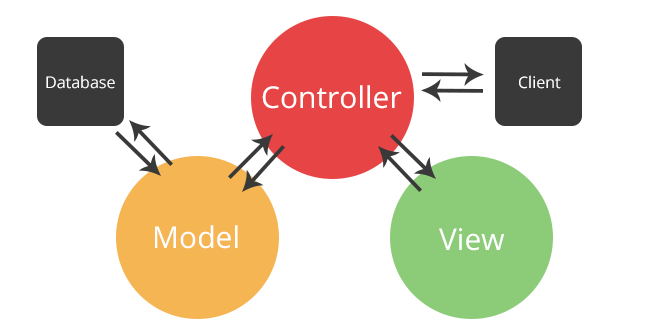
\includegraphics[width=\linewidth]{MVC}
    \caption{Modelo Vista-Controlador}
    
\end{figure}

Esta arquitectura permite estructurar la aplicación en tres capas y relacionarlas entre ellas:
\begin{itemize}
 \item \textbf{Modelo}: estructura interna de los datos (clases y modelos de las tablas de la base de datos).
 \item \textbf{Controlador}: clase que se encarga de obtener datos del modelo o de enviar estos al mismo. Es el puente entre la vista y los modelos.
 \item \textbf{Vista}: visualiza los datos del modelo que son enviados por el controlador, es la forma de interacción entre el cliente y el servidor, y se comunica de nuevo con el controlador para enviar peticiones o datos de vuelta al modelo. 
 \end{itemize}
 
El lado del modelo y el de las vistas se unen a través de llamadas por parte de ambos (redirecciones a las vistas, creación de modelos y acciones del controlador en el lado del controlador, y peticiones \emph{GET} y \emph{POST} desde el lado de las vistas).

La aplicación de este patrón funciona de la siguiente forma:
\begin{itemize}
    \item 1º. El controlador es el elemento principal, hace las redirecciones de las vistas y crea los modelos (objetos con elementos de la base de datos que se pasarán a la vistas para rellenar campos).
    \item 2º. El modelo es el elemento intermedio, se pasa a la vista para cargar los datos principales. Las vistas son la cara visible de la aplicación, de forma que el usuario puede editar o añadir datos en estas, y reenviarlos de nuevo al controlador.
    \item 3º. A través de peticiones \emph{GET} y \emph{POST} en las vistas, ya sea con formularios o con \emph{Ajax} (librería de JavaScript para hacer llamadas al controlador), la parte de la vista se comunica con el controlador y envía los datos.
\end{itemize}

\section{Diseño de Base de Datos}
Al trabajar con Core, a la hora de añadir/quitar/modificar tablas se realizará todo en code first. Code first es una forma de definir el modelo en dirección clase -> tabla, de forma que se define la estructura de la base de datos creando primero las clases del modelo o de las entidades que se utilizan en la aplicación. 

Los elementos necesarios para crear la estructura de la base de datos son los siguientes:
\begin{itemize}
    \item Clases/modelos de las tablas que se quieren añadir.
    \item Configuración de la cadena de conexión a la base de datos desde el archivo de configuración de la aplicación (appconfig.json, es un archivo que especifica, entre otros elementos, la cadena de conexión a la BD).
    \item Contexto de la aplicación (es un objeto del tipo Database Context que hace de nexo o puente entre el proyecto y la base de datos). El contexto se llena con las instancias de las clases que vamos a crear, y estas se migran a la base de datos a través de este.
    \item Consola del administrador de paquetes para migrar (añadir todos los nuevos cambios a la base de datos) y actualizar las tablas de la base de datos.
\end{itemize}

Las migraciones en Core son la forma en la que se actualiza la base de datos con los nuevos cambios de clases/atributos. El proyecto tiene un \emph{Snapshot}, que es un fichero que guarda la estructura de la base de datos en su última actualización. Si cambiamos o añadimos una clase o una columna, la migración lo compara con la snapshot para saber qué se debe cambiar en la base de datos.

El orden que se sigue para crear o modificar la estructura de la base de datos es:
\begin{itemize}
    \item 1º. Creación de la clase del modelo/tabla que se quiere añadir.
    \item 2º. Instancia de esta clase en el contexto de la aplicación.
    \item 3º. Con la consola del instalador de paquetes, añadir la migración.
    \item 4º. Después de la migración, actualizar la base de datos.
\end{itemize}

\section{Tablas/Modelos de la base de datos}
A continuación se muestran las tablas de la base de datos, con la notación DBM (DataBase Model):

\begin{table}[H]
    \centering
	\begin{tabularx}{\linewidth}{ p{0.25\columnwidth} p{0.61\columnwidth} }
		\textbf{DBM-01}    & \textbf{AptitudCV}\\
		\toprule
		\text{Descripción} & Tabla para almacenar las entradas de Aptitud de los CV's \\		
		\toprule
        \textbf{Campo}          & \textbf{Tipo}\\
        \text{IdAptitudCV}      & int (PK) \\	
        \text{Descripcion}      & nvarchar(max) null \\	
        \text{IdCurriculum}     & int (FK - Curriculum) null\\	
		\bottomrule
	\end{tabularx}
	\caption{DBM-01 AptitudCV}
\end{table}

\begin{table}[H]
    \centering
	\begin{tabularx}{\linewidth}{ p{0.25\columnwidth} p{0.61\columnwidth} }
		\textbf{DBM-02}    & \textbf{Curriculum}\\
		\toprule
		\text{Descripción} & Tabla para almacenar los currículums \\		
		\toprule
        \textbf{Campo}          & \textbf{Tipo}\\
        \text{IdCurriculum}     & int (PK) \\	
        \text{IdUsuario}        & int not null \\	
        \text{FechaCurriculum}  & datetime null \\	
		\bottomrule
	\end{tabularx}
	\caption{DBM-02 Curriculum}
\end{table}

\begin{table}[H]
    \centering
	\begin{tabularx}{\linewidth}{ p{0.25\columnwidth} p{0.6\columnwidth} }
		\textbf{DBM-03}    & \textbf{Departamento}\\
		\toprule
		\text{Descripción} & Tabla maestra de departamentos \\		
		\toprule
        \textbf{Campo}          & \textbf{Tipo}\\
        \text{IdDepartamento}   & int (PK) \\	
        \text{Descripcion}      & nvarchar(50) not null \\	
        \text{Codigo}           & nvarchar(max) null \\	
		\bottomrule
	\end{tabularx}
	\caption{DBM-03 Departamento}
\end{table}

\begin{table}[H]
    \centering
	\begin{tabularx}{\linewidth}{ p{0.25\columnwidth} p{0.60\columnwidth} }
		\textbf{DBM-04}    & \textbf{Entrada}\\
		\toprule
		\text{Descripción} & Tabla para guardar las publicaciones de los usuarios \\		
		\toprule
        \textbf{Campo}          & \textbf{Tipo}\\
        \text{IdEntrada}        & int (PK) \\	
        \text{IdUsuario}        & int (FK - Usuario) not null \\	
        \text{IdProyecto}       & int (FK - Proyecto) nulll \\	
        \text{Lenguaje}         & nvarchar(10) null \\
        \text{TituloIssue}      & nvarchar(50) null \\
        \text{Descripcion}      & nvarchar(150) not null \\
        \text{Editada}          & bit not null \\
        \text{Resuelta}         & bit not null \\
        \text{NumRespuestas}    & int null \\
		\bottomrule
	\end{tabularx}
	\caption{DBM-04 Entrada}
\end{table}

\begin{table}[H]
    \centering
	\begin{tabularx}{\linewidth}{ p{0.25\columnwidth} p{0.61\columnwidth} }
		\textbf{DBM-05}    & \textbf{EntradaCV}\\
		\toprule
		\text{Descripción} & Tabla que guarda la experiencia laboral 
                               de los usuarios de los CV's \\		
		\toprule
        \textbf{Campo}          & \textbf{Tipo}\\
        \text{IdEntradaCV}      & int (PK) \\	
        \text{IdUsuario}        & int (FK - Usuario) null\\	
        \text{IdCurriculum}     & int (FK - Curriculum) null\\	
        \text{Observaciones}    & nvarchar(max) not null \\	
        \text{PuestoTrabajo}    & nvarchar(50) null\\	
        \text{EmpresaAsociada}  & nvarchar(50) null \\	
        \text{Ubicacion}        & nvarchar(max) null \\	
        \text{FechaDesde}       & datetime not null \\	
        \text{FechaHasta}       & datetime not null \\	
		\bottomrule
	\end{tabularx}
	\caption{DBM-05 EntradaCV}
\end{table}

\begin{table}[H]
    \centering
	\begin{tabularx}{\linewidth}{ p{0.25\columnwidth} p{0.61\columnwidth} }
		\textbf{DBM-06}    & \textbf{FormacionCV}\\
		\toprule
		\text{Descripción} & Tabla que guarda la formacion académica 
                               de los usuarios de los CV's \\		
		\toprule
        \textbf{Campo}          & \textbf{Tipo}\\
        \text{IdFormacionCV}    & int (PK) \\	
        \text{IdUsuario}        & int (FK - Usuario) null\\	
        \text{IdCurriculum}     & int (FK - Curriculum) null\\	
        \text{IdTipoFormacion}  & int (FK - TipoFormacion) null\\	
        \text{Grado}            & nvarchar(max) not null \\	
        \text{Descripcion}      & nvarchar(max) null\\	
        \text{Ubicacion}        & nvarchar(max) null \\	
        \text{FechaDesde}       & datetime null \\	
        \text{FechaHasta}       & datetime null \\	
		\bottomrule
	\end{tabularx}
	\caption{DBM-06 FormacionCV}
\end{table}

\begin{table}[H]
    \centering
	\begin{tabularx}{\linewidth}{ p{0.25\columnwidth} p{0.61\columnwidth} }
		\textbf{DBM-07}    & \textbf{EventosUsuario}\\
		\toprule
		\text{Descripción} & Tabla que guarda los eventos programados de los usuarios \\		
		\toprule
        \textbf{Campo}          & \textbf{Tipo}\\
        \text{IdEventoUsuario}  & int (PK) \\	
        \text{IdUsuario}        & int (FK - Usuario) null\\	
        \text{Descripción}      & nvarchar(50) not null \\		
		\bottomrule
	\end{tabularx}
	\caption{DBM-07 EventosUsuario}
\end{table}

\begin{table}[H]
    \centering
	\begin{tabularx}{\linewidth}{ p{0.25\columnwidth} p{0.61\columnwidth} }
		\textbf{DBM-08}    & \textbf{FotoUsuarioCV}\\
		\toprule
		\text{Descripción} & Tabla que guarda la foto de usuario de un currículum
                               específico de un usuario\\		
		\toprule
        \textbf{Campo}          & \textbf{Tipo}\\
        \text{IdFotoUsuarioCV}  & int (PK) \\	
        \text{IdUsuario}        & int (FK - Usuario) null\\	
        \text{IdCurriculum}     & int (FK - Curriculum) null\\	
        \text{Ruta}             & nvarchar(max) null \\	
        \text{Guid}             & nvarchar(36) null\\	
        \text{Ext}              & nvarchar(max) null \\	
		\bottomrule
	\end{tabularx}
	\caption{DBM-08 FotoUsuarioCV}
\end{table}

\begin{table}[H]
    \centering
	\begin{tabularx}{\linewidth}{ p{0.25\columnwidth} p{0.61\columnwidth} }
		\textbf{DBM-09}    & \textbf{Grupo}\\
		\toprule
		\text{Descripción} & Tabla maestra para los grupos\\		
		\toprule
        \textbf{Campo}          & \textbf{Tipo}\\
        \text{IdGrupo}          & int (PK) \\	
        \text{Descripcion}      & nvarchar(50) null \\	
		\bottomrule
	\end{tabularx}
	\caption{DBM-09 Grupo}
\end{table}

\begin{table}[H]
    \centering
	\begin{tabularx}{\linewidth}{ p{0.25\columnwidth} p{0.61\columnwidth} }
		\textbf{DBM-10}    & \textbf{Idioma}\\
		\toprule
		\text{Descripción} & Tabla maestra para los idiomas \\		
		\toprule
        \textbf{Campo}          & \textbf{Tipo}\\
        \text{IdIdioma}         & int (PK) \\	
        \text{Descripcion}      & nvarchar(50) not null \\	
        \text{Codigo}           & nvarchar(5) not null \\	
		\bottomrule
	\end{tabularx}
	\caption{DBM-10 Idioma}
\end{table}

\begin{table}[H]
    \centering
	\begin{tabularx}{\linewidth}{ p{0.25\columnwidth} p{0.61\columnwidth} }
		\textbf{DBM-11}    & \textbf{IdiomaCV}\\
		\toprule
		\text{Descripción} & Tabla que guarda las entradas de los idiomas de un usuario
                               de un currículum específico\\		
		\toprule
        \textbf{Campo}          & \textbf{Tipo}\\
        \text{IdIdiomaCV}       & int (PK) \\
        \text{IdIdioma}         & int (FK - Idioma) null \\
        \text{IdNivelIdioma}    & int (FK - NivelIdioma) null \\
        \text{IdCurriculum}     & int (FK - Curriculum) null \\        
        \text{Descripcion}      & nvarchar(max) not null \\	
        \text{Centro}           & nvarchar(50) not null \\	
        \text{FechaDesde}       & datetime null \\	
        \text{FechaHasta}       & datetime null \\	        
		\bottomrule
	\end{tabularx}
	\caption{DBM-11 IdiomaCV}
\end{table}

\begin{table}[H]
    \centering
	\begin{tabularx}{\linewidth}{ p{0.25\columnwidth} p{0.61\columnwidth} }
		\textbf{DBM-12}    & \textbf{LogroCV}\\
		\toprule
		\text{Descripción} & Tabla para almacenar las entradas de Logro de los CV's \\		
		\toprule
        \textbf{Campo}          & \textbf{Tipo}\\
        \text{IdLogroCV}        & int (PK) \\	
        \text{Descripcion}      & nvarchar(max) null \\	
        \text{IdCurriculum}     & int (FK - Curriculum) null\\	
		\bottomrule
	\end{tabularx}
	\caption{DBM-12 LogroCV}
\end{table}

\begin{table}[H]
    \centering
	\begin{tabularx}{\linewidth}{ p{0.25\columnwidth} p{0.61\columnwidth} }
		\textbf{DBM-13}    & \textbf{NivelIdioma}\\
		\toprule
		\text{Descripción} & Tabla maestra con los niveles de los idiomas \\		
		\toprule
        \textbf{Campo}          & \textbf{Tipo}\\
        \text{IdNivelIdioma}    & int (PK) \\	
        \text{Descripcion}      & nvarchar(50) not null \\	
		\bottomrule
	\end{tabularx}
	\caption{DBM-13 NivelIdioma}
\end{table}

\begin{table}[H]
    \centering
	\begin{tabularx}{\linewidth}{ p{0.25\columnwidth} p{0.61\columnwidth} }
		\textbf{DBM-14}    & \textbf{NotasUsuario}\\
		\toprule
		\text{Descripción} & Tabla para almacenar las notas de usuario \\		
		\toprule
        \textbf{Campo}          & \textbf{Tipo}\\
        \text{IdNotaUsuario}    & int (PK) \\	
        \text{IdUsuario}        & int (FK - Usuario) not null \\	
        \text{Descripcion}      & nvarchar(100) null\\	
        \text{Titulo}      & nvarchar(50) not null\\	
		\bottomrule
	\end{tabularx}
	\caption{DBM-14 NotasUsuario}
\end{table}

\begin{table}[H]
    \centering
	\begin{tabularx}{\linewidth}{ p{0.25\columnwidth} p{0.61\columnwidth} }
		\textbf{DBM-15}    & \textbf{Notificacion}\\
		\toprule
		\text{Descripción} & Tabla para las notificaciones de los usuarios por eventos
                               o respuestas\\		
		\toprule
        \textbf{Campo}              & \textbf{Tipo}\\
        \text{IdNotificacion}       & int (PK) \\	
        \text{IdTipoNotificacion}   & int (FK - TipoNotificacion) not null \\	
        \text{IdUsuario}            & int (FK - Usuario) not null \\	
        \text{Descripcion}          & nvarchar(100) null\\	
        \text{Leido}                & bit not null\\	
		\bottomrule
	\end{tabularx}
	\caption{DBM-15 Notificacion}
\end{table}

\begin{table}[H]
    \centering
	\begin{tabularx}{\linewidth}{ p{0.25\columnwidth} p{0.61\columnwidth} }
		\textbf{DBM-16}    & \textbf{Proyecto}\\
		\toprule
		\text{Descripción} & Tabla maestra con los proyectos de la empresa \\		
		\toprule
        \textbf{Campo}              & \textbf{Tipo}\\
        \text{IdProyecto}           & int (PK) \\		
        \text{Descripcion}          & nvarchar(100) null\\	
		\bottomrule
	\end{tabularx}
	\caption{DBM-16 Proyecto}
\end{table}

\begin{table}[H]
    \centering
	\begin{tabularx}{\linewidth}{ p{0.25\columnwidth} p{0.61\columnwidth} }
		\textbf{DBM-17}    & \textbf{Respuesta}\\
		\toprule
		\text{Descripción} & Tabla para respuestas a publicaciones de usuarios \\		
		\toprule
        \textbf{Campo}              & \textbf{Tipo}\\
        \text{IdRespuesta}          & int (PK) \\	
        \text{IdEntrada}            & int (FK - Entrada) not null \\	
        \text{IdUsuario}            & int (FK - Usuario) not null \\	
        \text{Descripcion}          & nvarchar(100) not null\\	
        \text{UpVotes}              & int not null\\	
		\bottomrule
	\end{tabularx}
	\caption{DBM-17 Respuesta}
\end{table}

\begin{table}[H]
    \centering
	\begin{tabularx}{\linewidth}{ p{0.25\columnwidth} p{0.61\columnwidth} }
		\textbf{DBM-18}    & \textbf{Rol}\\
		\toprule
		\text{Descripción} & Tabla maestra con los roles de la empresa \\		
		\toprule
        \textbf{Campo}              & \textbf{Tipo}\\
        \text{IdRol}                & int (PK) \\		
        \text{Descripcion}          & nvarchar(50) not null\\	
		\bottomrule
	\end{tabularx}
	\caption{DBM-18 Rol}
\end{table}

\begin{table}[H]
    \centering
	\begin{tabularx}{\linewidth}{ p{0.25\columnwidth} p{0.61\columnwidth} }
		\textbf{DBM-19}    & \textbf{TipoEntrada}\\
		\toprule
		\text{Descripción} & Tabla maestra con los tipos de publicaciones \\		
		\toprule
        \textbf{Campo}              & \textbf{Tipo}\\
        \text{IdTipoEntrada}        & int (PK) \\		
        \text{Descripcion}          & nvarchar(50) not null\\	
		\bottomrule
	\end{tabularx}
	\caption{DBM-19 TipoEntrada}
\end{table}

\begin{table}[H]
    \centering
	\begin{tabularx}{\linewidth}{ p{0.25\columnwidth} p{0.61\columnwidth} }
		\textbf{DBM-20}    & \textbf{TipoFormacion}\\
		\toprule
		\text{Descripción} & Tabla maestra con los tipos de formacion en los currículums \\		
		\toprule
        \textbf{Campo}              & \textbf{Tipo}\\
        \text{IdTipoFormacion}      & int (PK) \\		
        \text{Descripcion}          & nvarchar(50) not null\\	
		\bottomrule
	\end{tabularx}
	\caption{DBM-20 TipoFormacion}
\end{table}

\begin{table}[H]
    \centering
	\begin{tabularx}{\linewidth}{ p{0.25\columnwidth} p{0.61\columnwidth} }
		\textbf{DBM-21}    & \textbf{TipoNotificacion}\\
		\toprule
		\text{Descripción} & Tabla maestra con los tipos de notificaciones de la aplicación \\		
		\toprule
        \textbf{Campo}              & \textbf{Tipo}\\
        \text{IdTipoNotificacion}   & int (PK) \\		
        \text{Descripcion}          & nvarchar(50) not null\\	
		\bottomrule
	\end{tabularx}
	\caption{DBM-21 TipoNotificacion}
\end{table}

\begin{table}[H]
    \centering
	\begin{tabularx}{\linewidth}{ p{0.25\columnwidth} p{0.61\columnwidth} }
		\textbf{DBM-22}    & \textbf{Usuario}\\
		\toprule
		\text{Descripción} & Tabla de los usuarios registrados en el sistema \\		
		\toprule
        \textbf{Campo}              & \textbf{Tipo}\\
        \text{IdUsuario}            & int (PK) \\		
        \text{IdDepartamento}       & int (FK - Departamento) not null \\
        \text{IdGrupo}              & int (FK - Grupo) null \\
        \text{IdRol}                & int (FK - Rol) null \\
        \text{NombreUser}           & nvarchar(50) not null\\	
        \text{Nombre}               & nvarchar(50) null\\
        \text{Apellido}             & nvarchar(50) null\\
        \text{Password}             & nvarchar(max) not null\\
        \text{Foto}                 & nvarchar(max) null\\
        \text{Email}                & nvarchar(max) null\\
        \text{Activo}               & bit not null\\
        \text{EsAdmin}              & bit not null\\
        \text{Biografia}            & nvarchar(max) null\\
		\bottomrule
	\end{tabularx}
	\caption{DBM-22 Usuario}
\end{table}

\begin{table}[H]
    \centering
	\begin{tabularx}{\linewidth}{ p{0.25\columnwidth} p{0.61\columnwidth} }
		\textbf{DBM-23}    & \textbf{UsuarioCV}\\
		\toprule
		\text{Descripción} & Tabla de los datos principales del usuario en un currículum \\		
		\toprule
        \textbf{Campo}              & \textbf{Tipo}\\
        \text{IdUsuarioCV}          & int (PK) \\		
        \text{IdUsuario}            & int (FK - Usuario) not null \\
        \text{IdCurriculum}         & int (FK - Curriculum) not null \\
        \text{IdFotoUsuarioCV}      & int (FK - FotoUsuarioCV) null \\	
        \text{Nombre}               & nvarchar(50) null\\
        \text{Apellido1}            & nvarchar(50) null\\
        \text{Apellido2}            & nvarchar(50) null\\
        \text{Profesion}            & nvarchar(max) null\\
        \text{Nacionalidad}         & nvarchar(max) null\\
        \text{Email}                & nvarchar(max) null\\
        \text{Telefono}             & int null\\
        \text{EnlaceContacto}       & nvarchar(max) null\\
        \text{FechaNacimiento}      & datetime null\\
        \text{AcercaDe}             & nvarchar(max) null\\
		\bottomrule
	\end{tabularx}
	\caption{DBM-23 UsuarioCV}
\end{table}
\newpage
\section{Diagrama E/R}
A continuación se adjuntan las relaciones entre las distintas entidades de la aplicación.
\begin{figure}[H]
    \centering
    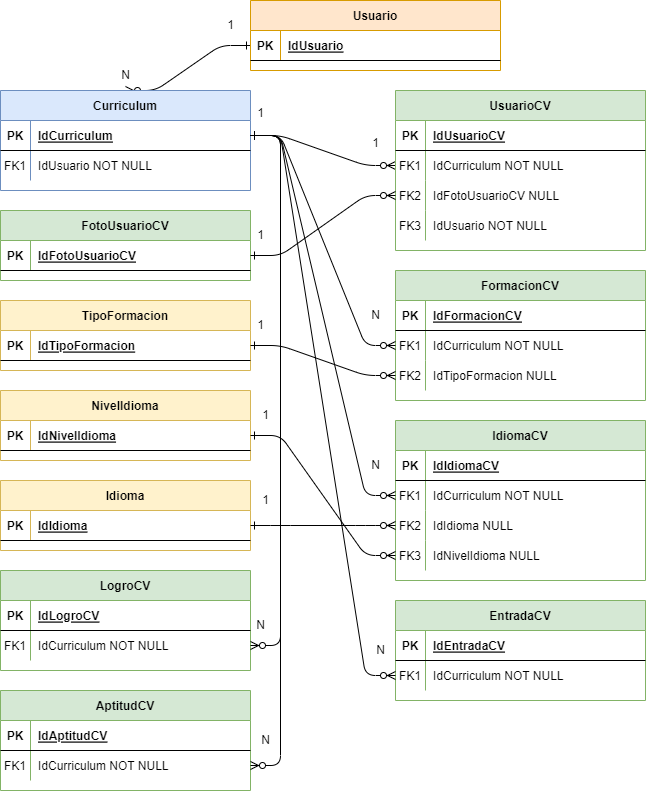
\includegraphics[width=\linewidth]{img/diagramaER_TFG.png}
    \caption{Diagrama ER - Currículos}  
\end{figure}

\begin{figure}[H]
    \centering
    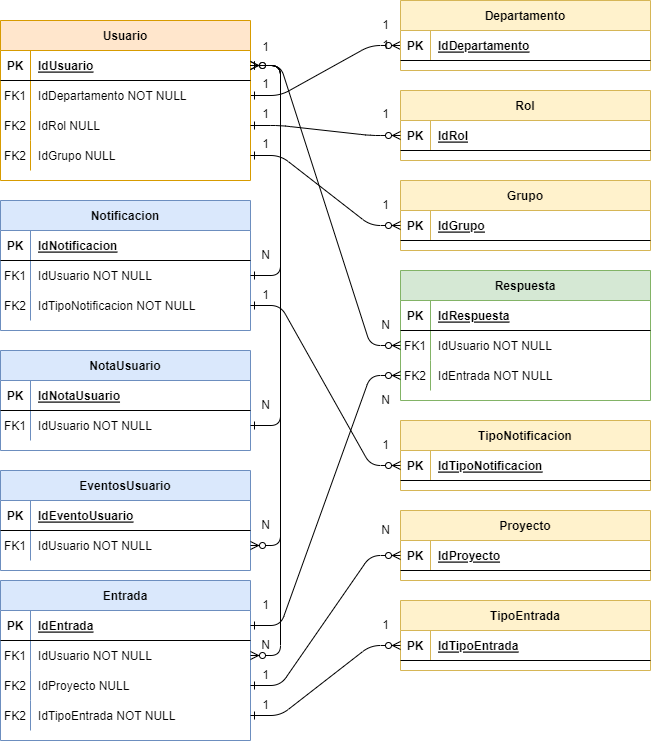
\includegraphics[width=\linewidth]{img/diagramaER2_TFG.png}
    \caption{Diagrama ER - Otros casos}  
\end{figure}

\section{Diseño estructural y funcional}
Para explicar el diseño interno de la aplicación, se va a dividir en dos categorías:
\begin{itemize}
    \item Estructura de proyectos y directorios.
    \item Instancia del programa, flujo y funcionalidad.
\end{itemize}

\subsection{Estructura interna}
La aplicación tiene los siguientes proyectos:
\begin{itemize}
    \item \textbf{Proyecto Web}: es el proyecto principal, en él se encuentra la instanciación
    de la aplicación y las configuraciones principales.
    \item \textbf{AccesoDatos}: proyecto que contiene los datos del contexto de la base de datos
    y los repositorios de los modelos para su actualización.
    \item \textbf{Modelos}: proyecto que contiene los modelos o clases referentes a la base
    de datos.
    \item \textbf{Exceptions}: proyecto del middleware de manejo de excepciones.
    \item \textbf{Logs}: en este directorio se guardan los logs de la aplicación.
    \item \textbf{Utilidades}: proyecto extra con clases comunes y/o globales.
\end{itemize}

\subsubsection{Proyecto web}
Como se ha explicado antes, es el proyecto principal. Por un lado, tiene los siguientes elementos:
\begin{itemize}
\tightlist
    \item Contiene el archivo principal de carga de la aplicación que es ``program.cs''.
    \item Tiene las configuraciones de la cadena de conexión en un ``appsettings.json''.
    \item Propiedades del lanzamiento de la aplicación (variables de entorno, puertos, etc.).
\end{itemize}

Además, posee los siguientes directorios:
\begin{itemize}
    \item \textbf{wwwroot}: carpeta root de la aplicación que contiene las hojas de estilos, scripts
    y otras carpetas de utilidad (imágenes, iconos y librerías).
    \item \textbf{Views}: carpeta contenedora de todas las vistas de la aplicación.
    \item \textbf{Controllers}: carpeta donde se guardan las clases de los controladores.
\end{itemize}

\subsubsection{AccesoDatos}
Es el proyecto que une el contexto de la base de datos con el programa, y tiene los siguientes subdirectorios:
\begin{itemize}
    \item \textbf{\emph{Data}}: contiene el archivo de instanciación del contexto y las tablas de la base de datos.
    \item \textbf{\emph{Migrations}}: guarda los cambios en la base de datos a través de migraciones y actualiza la imagen de la base de datos (este archivo contiene la estructura de la base de datos en cuanto a tablas y datos en forma de script en código de servidor).
    \item \textbf{Repositorio}: contiene las clases de los repositorios. Cada tabla tiene una
    para poder acceder a ella y cambiar u obtener datos. La instanciación depende de una interfaz
    que se realiza de la misma forma (una por cada tabla) y por último se añaden a un archivo global llamado ``UnitOfWork'', que es el medio por el que se obtienen las llamadas a dichas clases.
\end{itemize}

\subsubsection{Modelos}
Proyecto contenedor de dos partes principales del modelo:
\begin{itemize}
    \item \textbf{ViewModels}: son modelos personalizados, creados e instanciados a tiempo real
    por los controladores. Los datos se cargan como indica el programador y forman modelos cuyo
    uso principal es dotar de datos de varias tablas a una vista.
    \item \textbf{Models}: las clases de las tablas de la base de datos.
\end{itemize}

\subsection{Funcionalidad del flujo}
La funcionalidad de la aplicación sigue un flujo por pasos, a través de las dependencias entre proyectos:
\begin{itemize}
    \item 1º. Se hacen las configuraciones previas (entorno, cadena de conexión, etc).
    \item 2º. Se añaden las dependencias de los proyectos para acceder a la información de los datos de los modelos.
    \item 3º. Se configuran las librerías y los paquetes externos.
    \item 4º. Se añade el contexto de la base de datos y se añaden las vistas al lanzador.
    \item 5º. Se añaden al objeto lanzador de la aplicación las redirecciones http y la configuración básica de la web.
    \item 6º. Se indica la vista principal del lanzamiento y se ejecuta a través del entorno indicado. Si no se configuran más entornos, coge por defecto ``develop'', que es el entorno
    local.
\end{itemize}

A partir de este punto, la aplicación se ejecuta y se accede a la vista que se indica de inicio. En este momento, todo está cargado y el flujo sigue los pasos del MVC, de forma que el usuario interactúa con la vista y el controlador realizará las acciones pertinentes (redirecciones, peticiones http del tipo POST o GET, etc.).

\subsection{Dependencias y paquetes}
Todos los proyectos anteriormente mencionados tienen dependencias, no sólo entre sí, sino también a nivel de librerías. Cada proyecto guarda una relación con otro dependiendo del nivel de ejecución.

Por ejemplo, el proyecto principal depende de todos los demás, ya que es el que lanza la aplicación. Por otro lado, el proyecto de AccesoDatos solo depende de Modelos, que es al que debe llamar para obtener los datos de las tablas. Otros como Modelos, Exceptions y Utilidades, no dependen de ningún proyecto, ya que son proyectos maestros que permiten la ejecución del resto.

En cuanto a las librerías y dependencias de Microsoft y ASP.NET Core se utliza el administrador de paquetes de NuGet. NuGet es una herramienta que permite instalar versiones de dependencias que aportan funciones y librerías para su uso en determinados entornos. Por ejemplo, para poder trabajar con .NET en Core, necesitamos la dependencia del \emph{EntityFramework}, que es el que permite la instanciación del contexto de los modelos en el ámbito de Core.

Todas las librerías y dependencias de proyectos de forma interna (no entre proyectos) se administran y añaden a través de este instalador de paquetes. De la misma forma, para poder realizar migraciones con cambios a base de datos, también debemos utilizar NuGet, pero en este caso se hace a través de la consola de comandos y no a través del administrador.

\section{Diseño de las vistas y navegación}
Las vistas son la parte visual de la aplicación, y, a través de ellas, el usuario puede interactuar con el servidor. Para realizar las vistas, se ha diseñado una serie de prototipos iniciales que aporten una ligera idea de cómo se vería la aplicación

\subsection{Navegación por la web}
A continuación y para finalizar con la parte del diseño de la aplicación, se explicará cómo es la navegación por la web.
\begin{figure}[H]
    \centering
    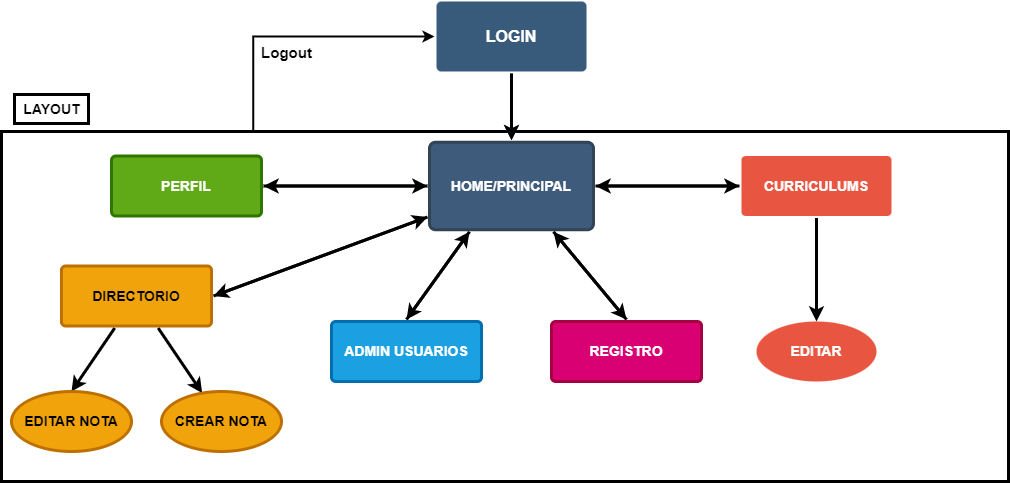
\includegraphics[width=\linewidth]{img/FlujoNavegacion.png}
    \caption{Navegación entre vistas de la aplicación}
\end{figure}


Hay varias vistas que tienen una navegación bidireccional, debido a que el layout permite:
\begin{itemize}
\tightlist
    \item Con el botón de logout volver al inicio de sesión.
    \item Volver a la página principal a través de ``Home''.
\end{itemize}

La estructura de la navegación se puede resumir en:
\begin{itemize}
\tightlist
    \item 1. \emph{Login} o inicio de sesión: vista madre de todas las demás, primera pantalla que se ve al iniciar.
    \item 2. \emph{Home}: página principal después del inicio y contenedora del layout (es el main).
    \item 3. Vistas secundarias como el perfil, los directorios, los currículums, la administración y el registro.
    \item 4. Otras vistas que se acceden a través de las anteriores, como la creación de notas y currículums, la edición de ambos, etc.
\end{itemize}


\subsection{Prototipos}
Los siguientes prototipos fueron diseñados en la fase de análisis, y forman las vistas principales de la aplicación (que no son todas, ya que muchas de las que hay en la versión final se fueron añadiendo sobre la marcha).

\begin{figure}
    \centering
    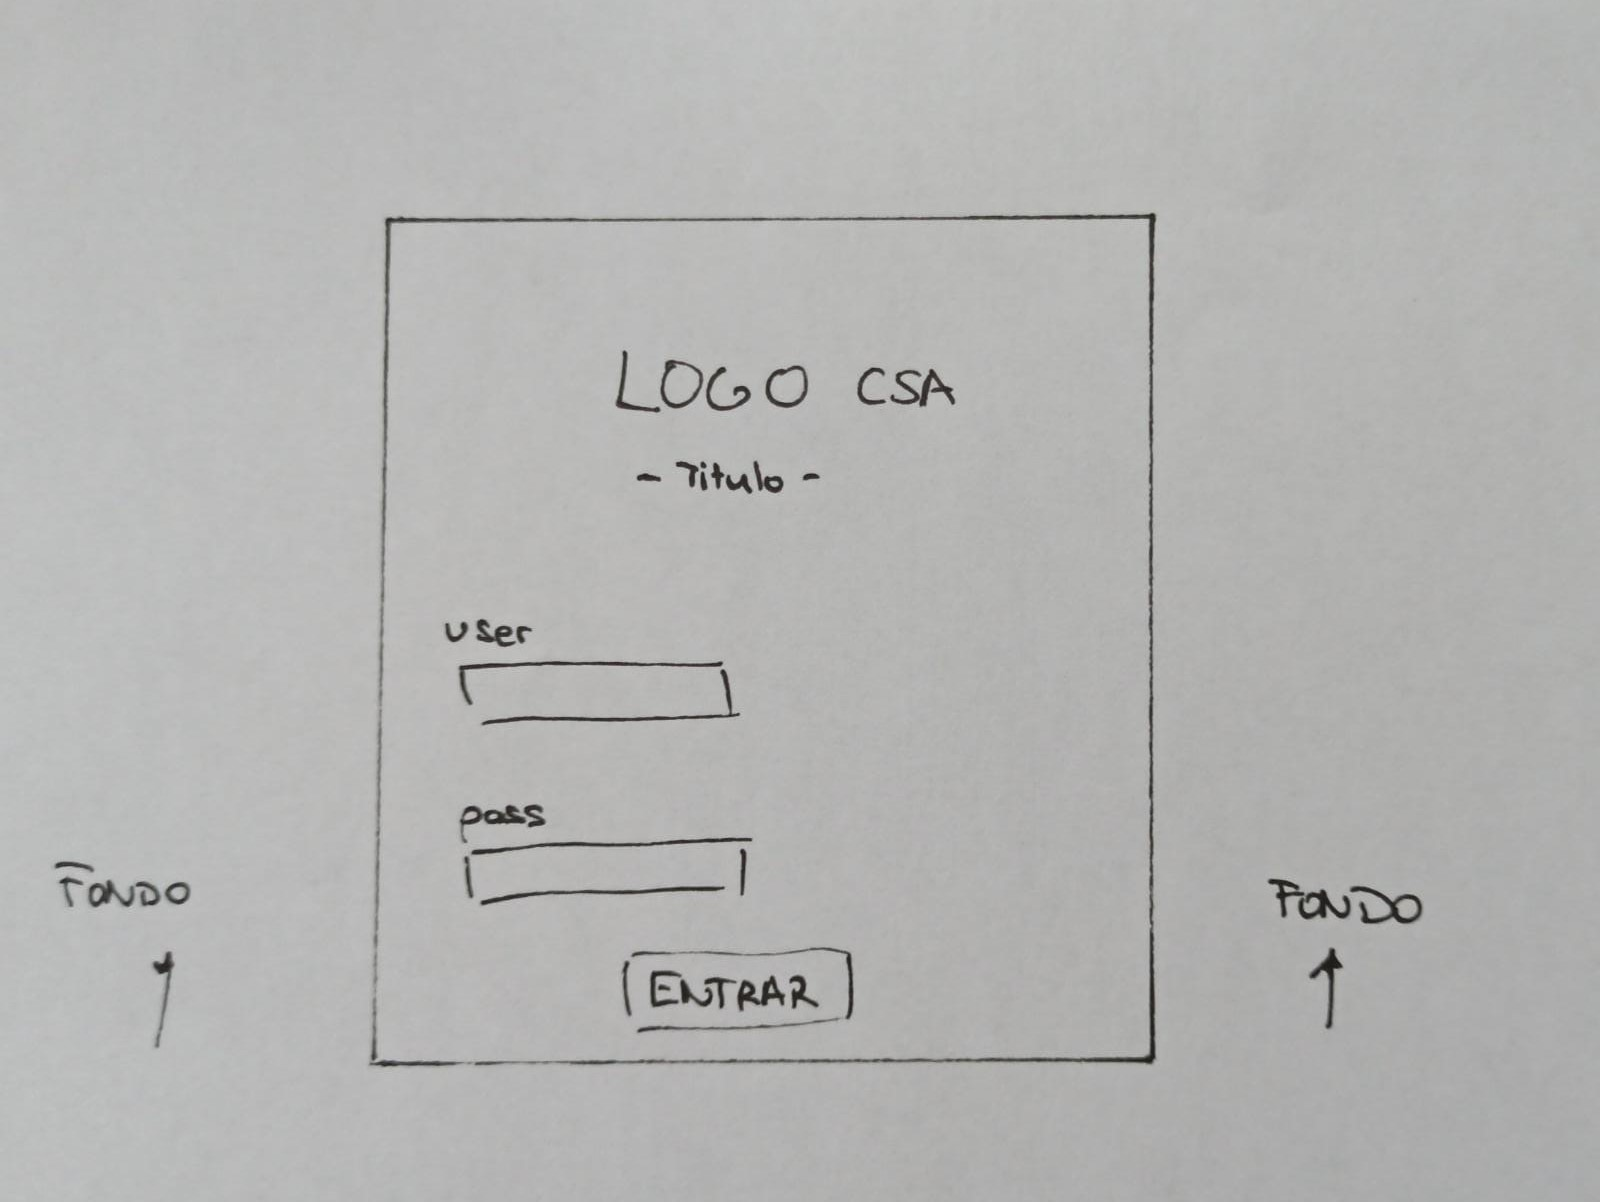
\includegraphics[width=\linewidth]{img/PT01-Login.jpeg}
    \caption{Prototipo 01. Vista del inicio de sesión}    
\end{figure}

\begin{figure}
    \centering
    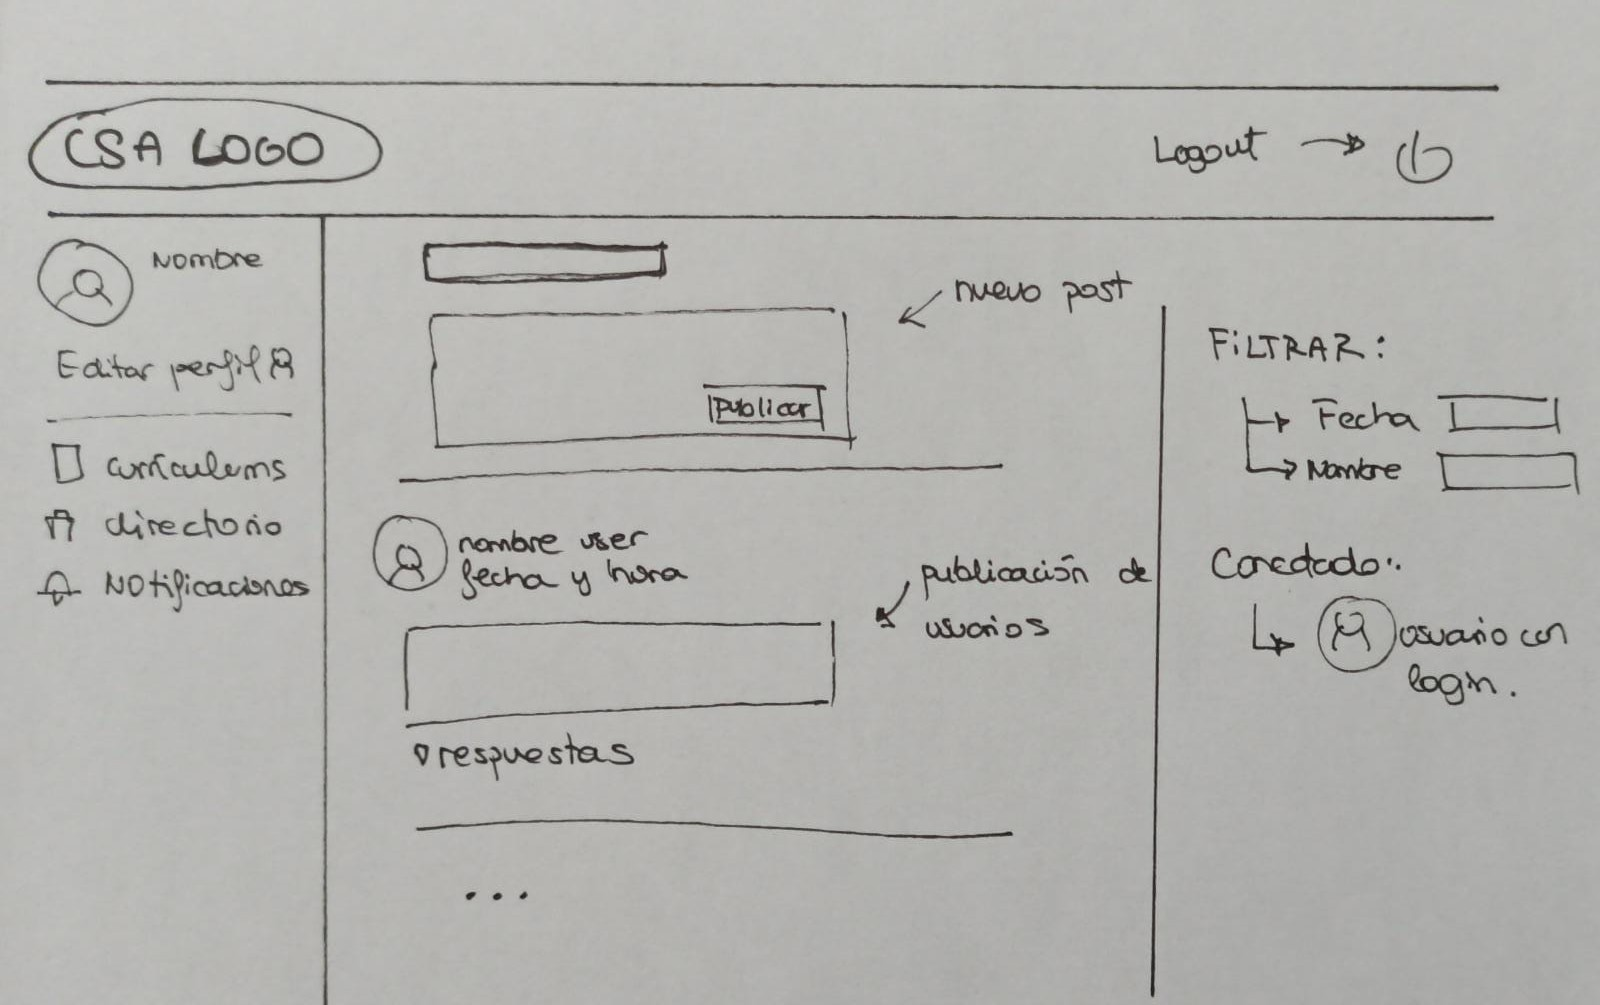
\includegraphics[width=\linewidth]{img/PT02-Home.jpeg}
    \caption{Prototipo 02. Vista principal y layout}   
\end{figure}

\begin{figure}
    \centering
    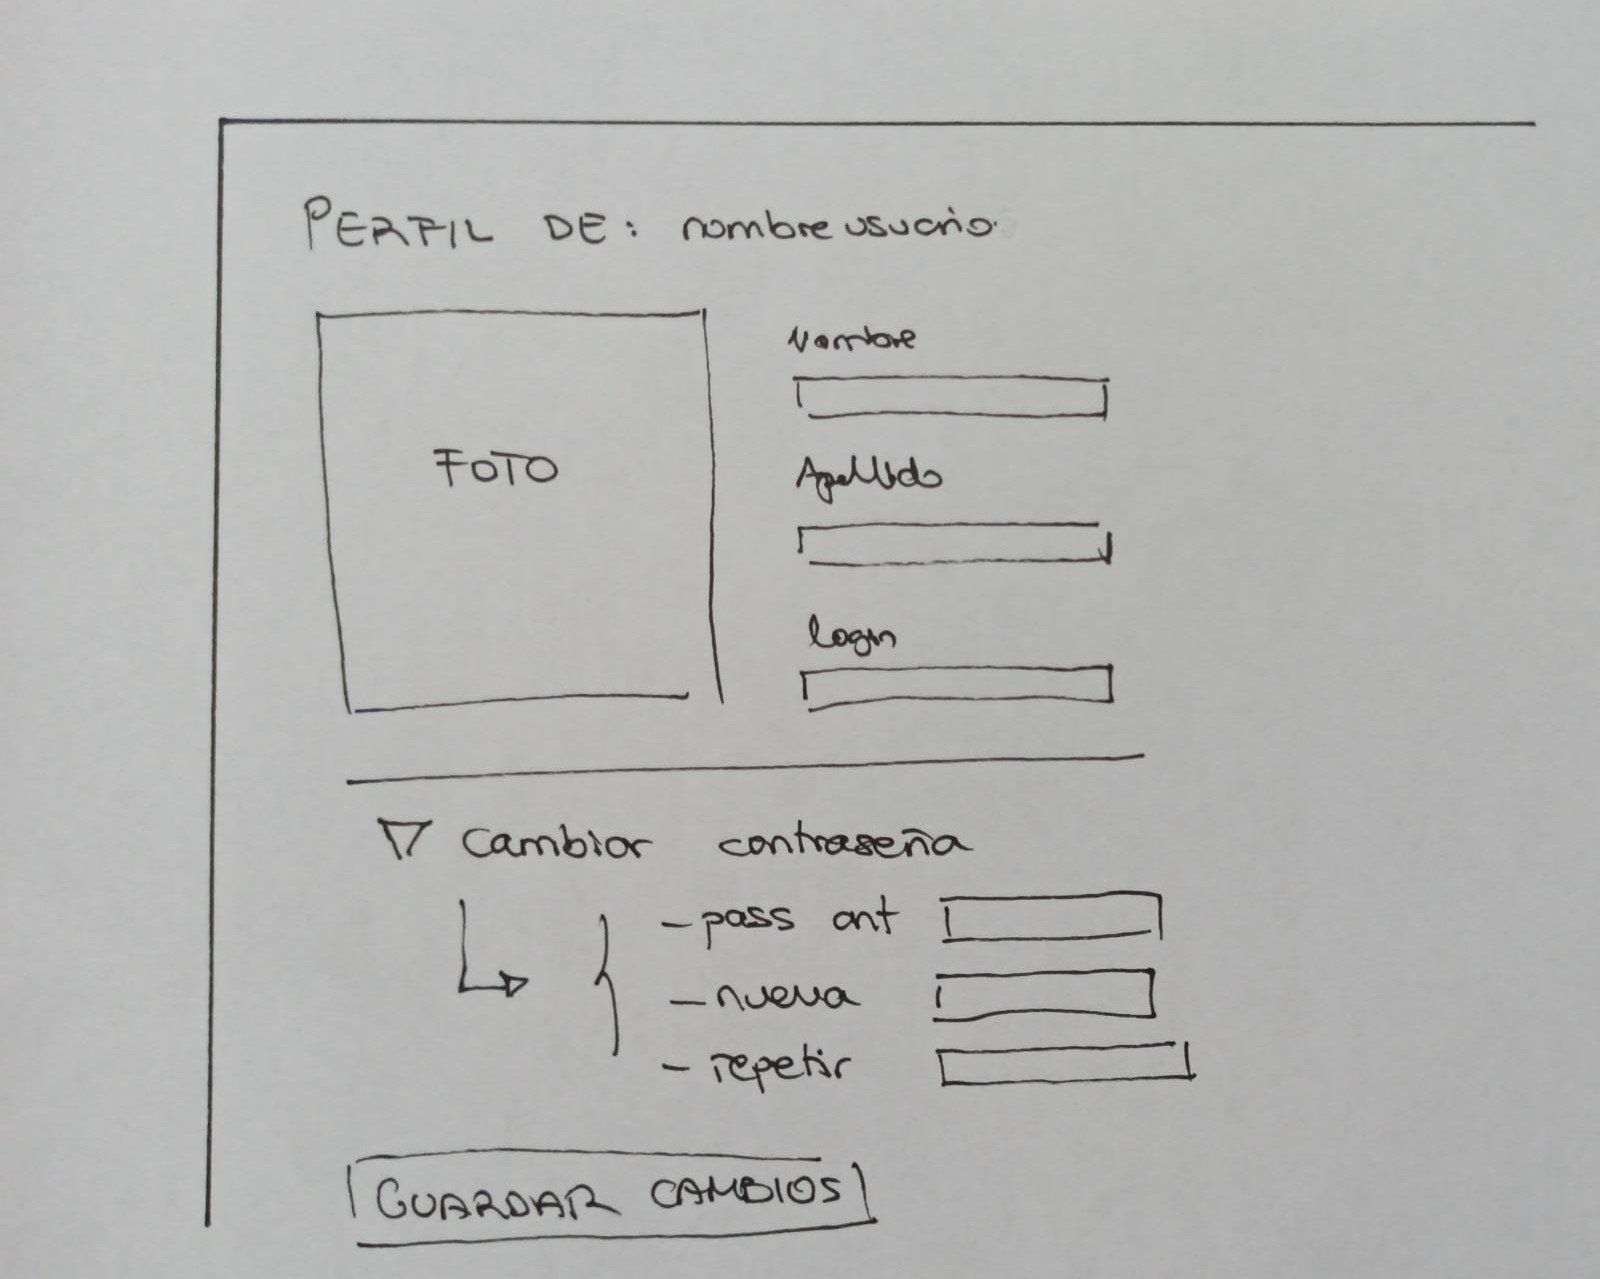
\includegraphics[width=\linewidth]{img/PT03-Profile.jpeg}
    \caption{Prototipo 03. Vista del perfil de los usuarios}    
\end{figure}

\begin{figure}
    \centering
    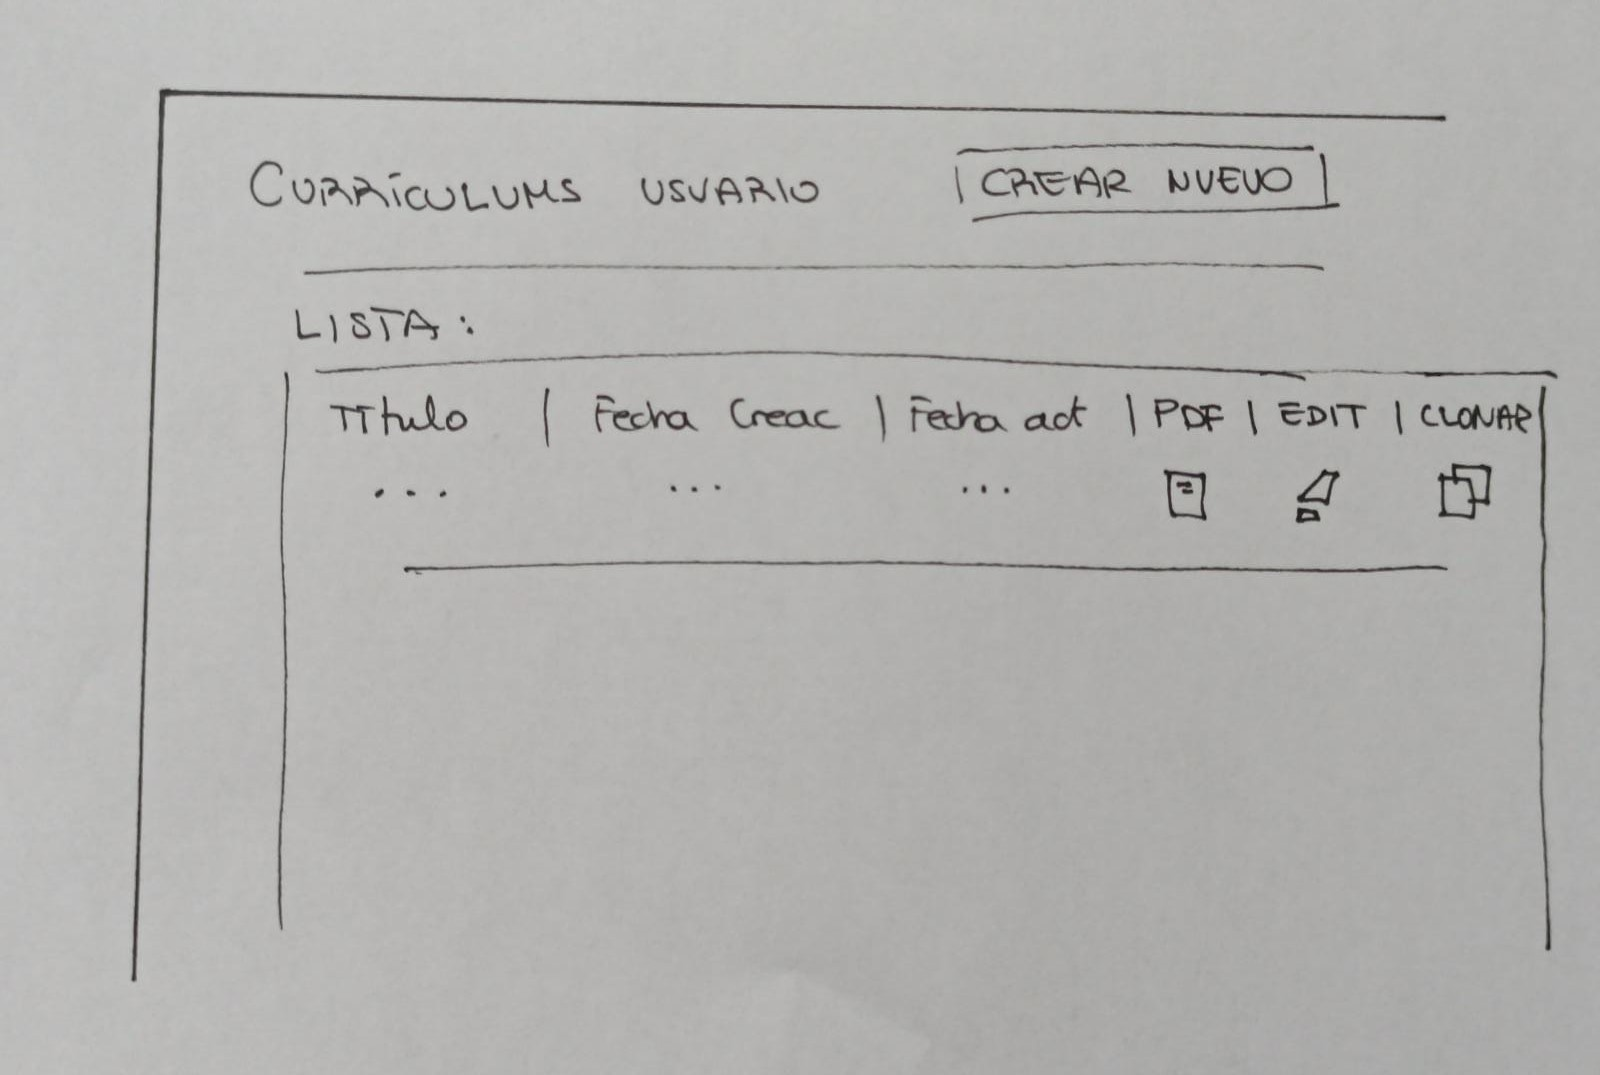
\includegraphics[width=\linewidth]{img/PT04-CVUser.jpeg}
    \caption{Prototipo 04. Vista de los currículums del usuario genérico}   
\end{figure}

\begin{figure}
    \centering
    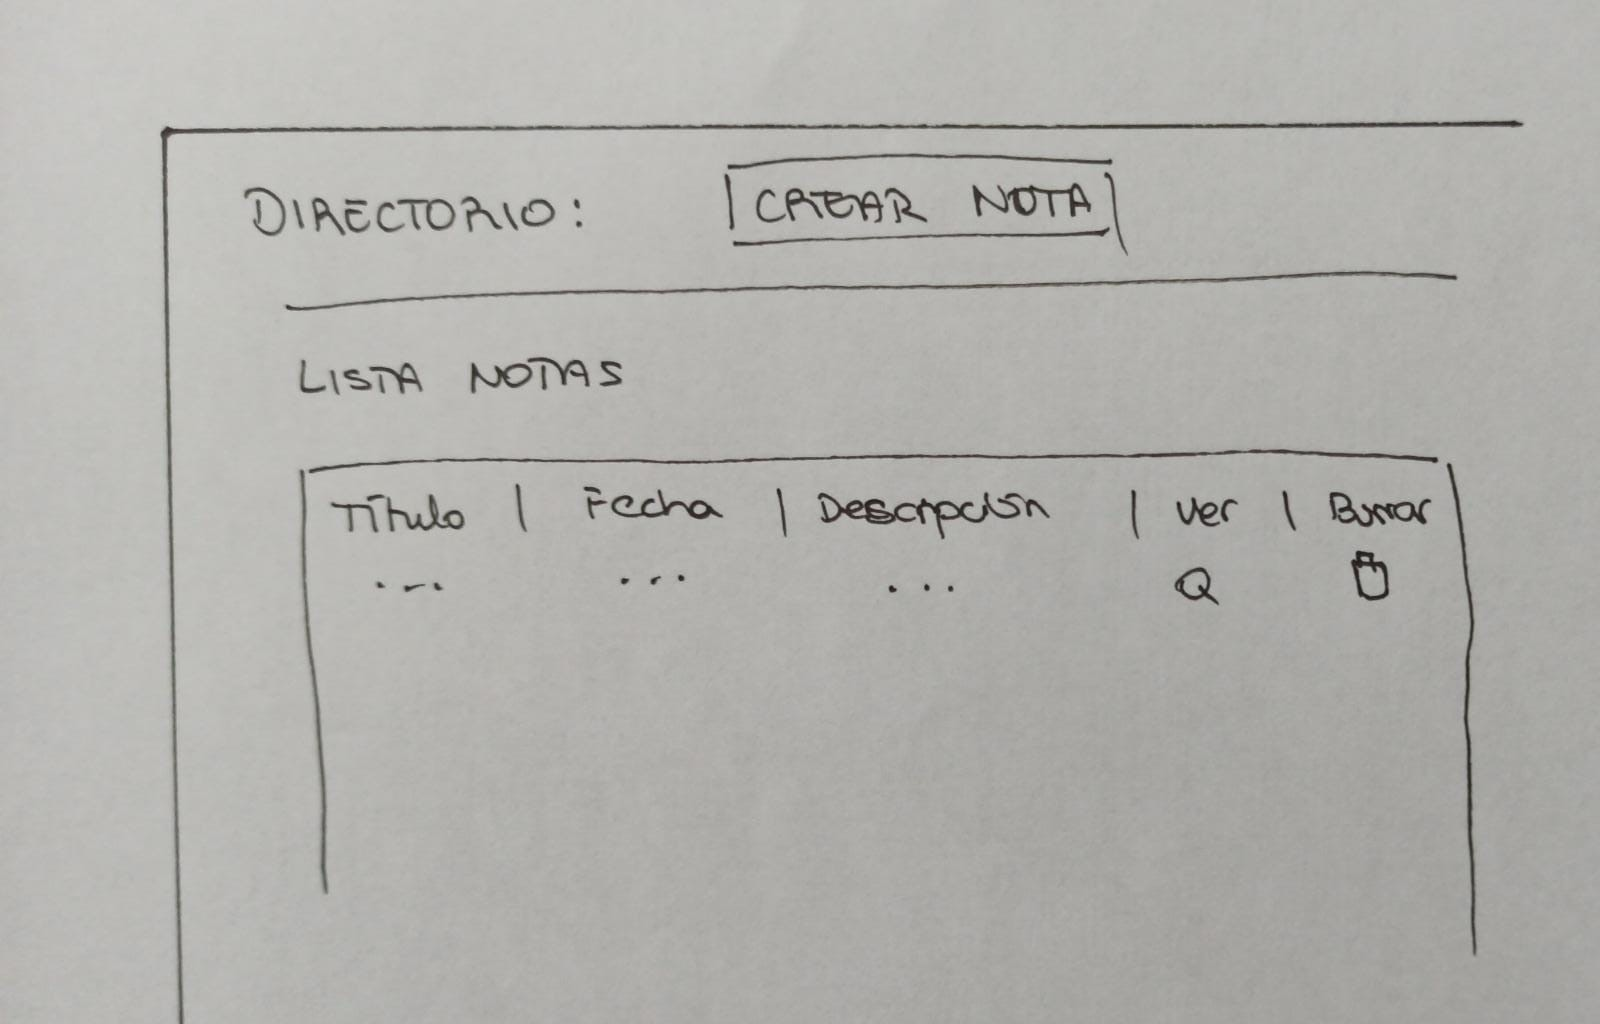
\includegraphics[width=\linewidth]{img/PT05-Directorio.jpeg}
    \caption{Prototipo 05. Vista del directorio de usuarios}
\end{figure}

\begin{figure}
    \centering
    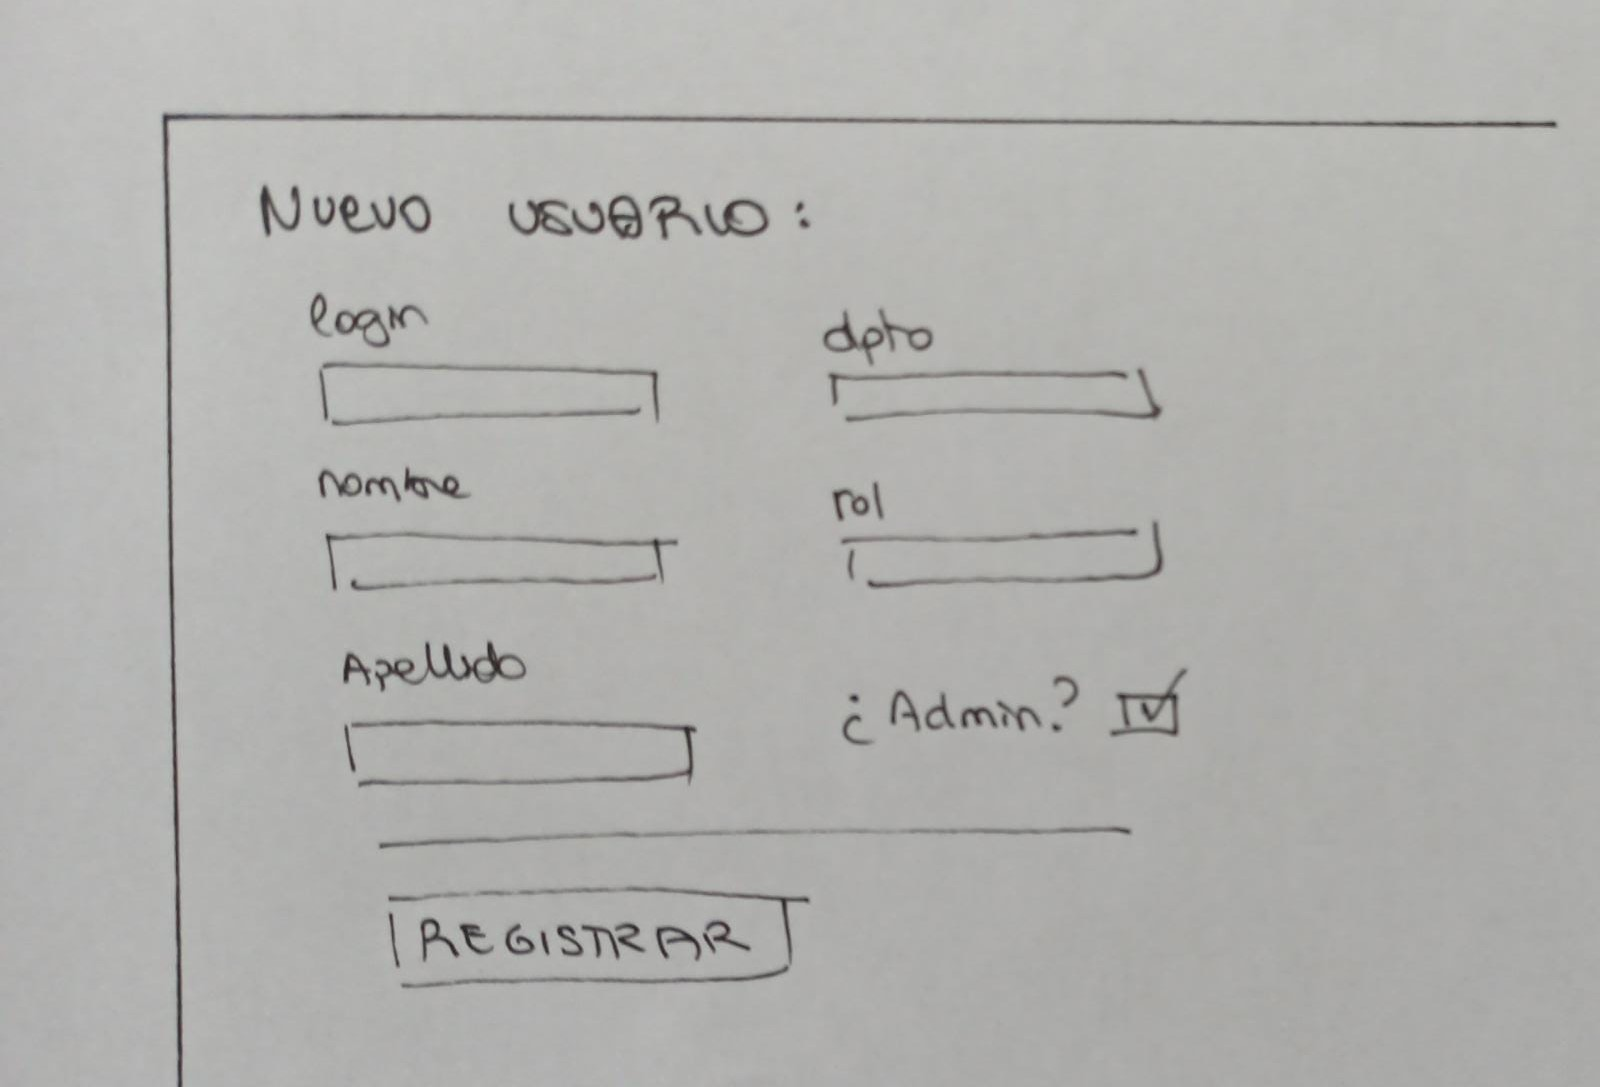
\includegraphics[width=\linewidth]{img/PT06-Register.jpeg}
    \caption{Prototipo 06. Vista del registro de usuarios}   
\end{figure}

\begin{figure}
    \centering
    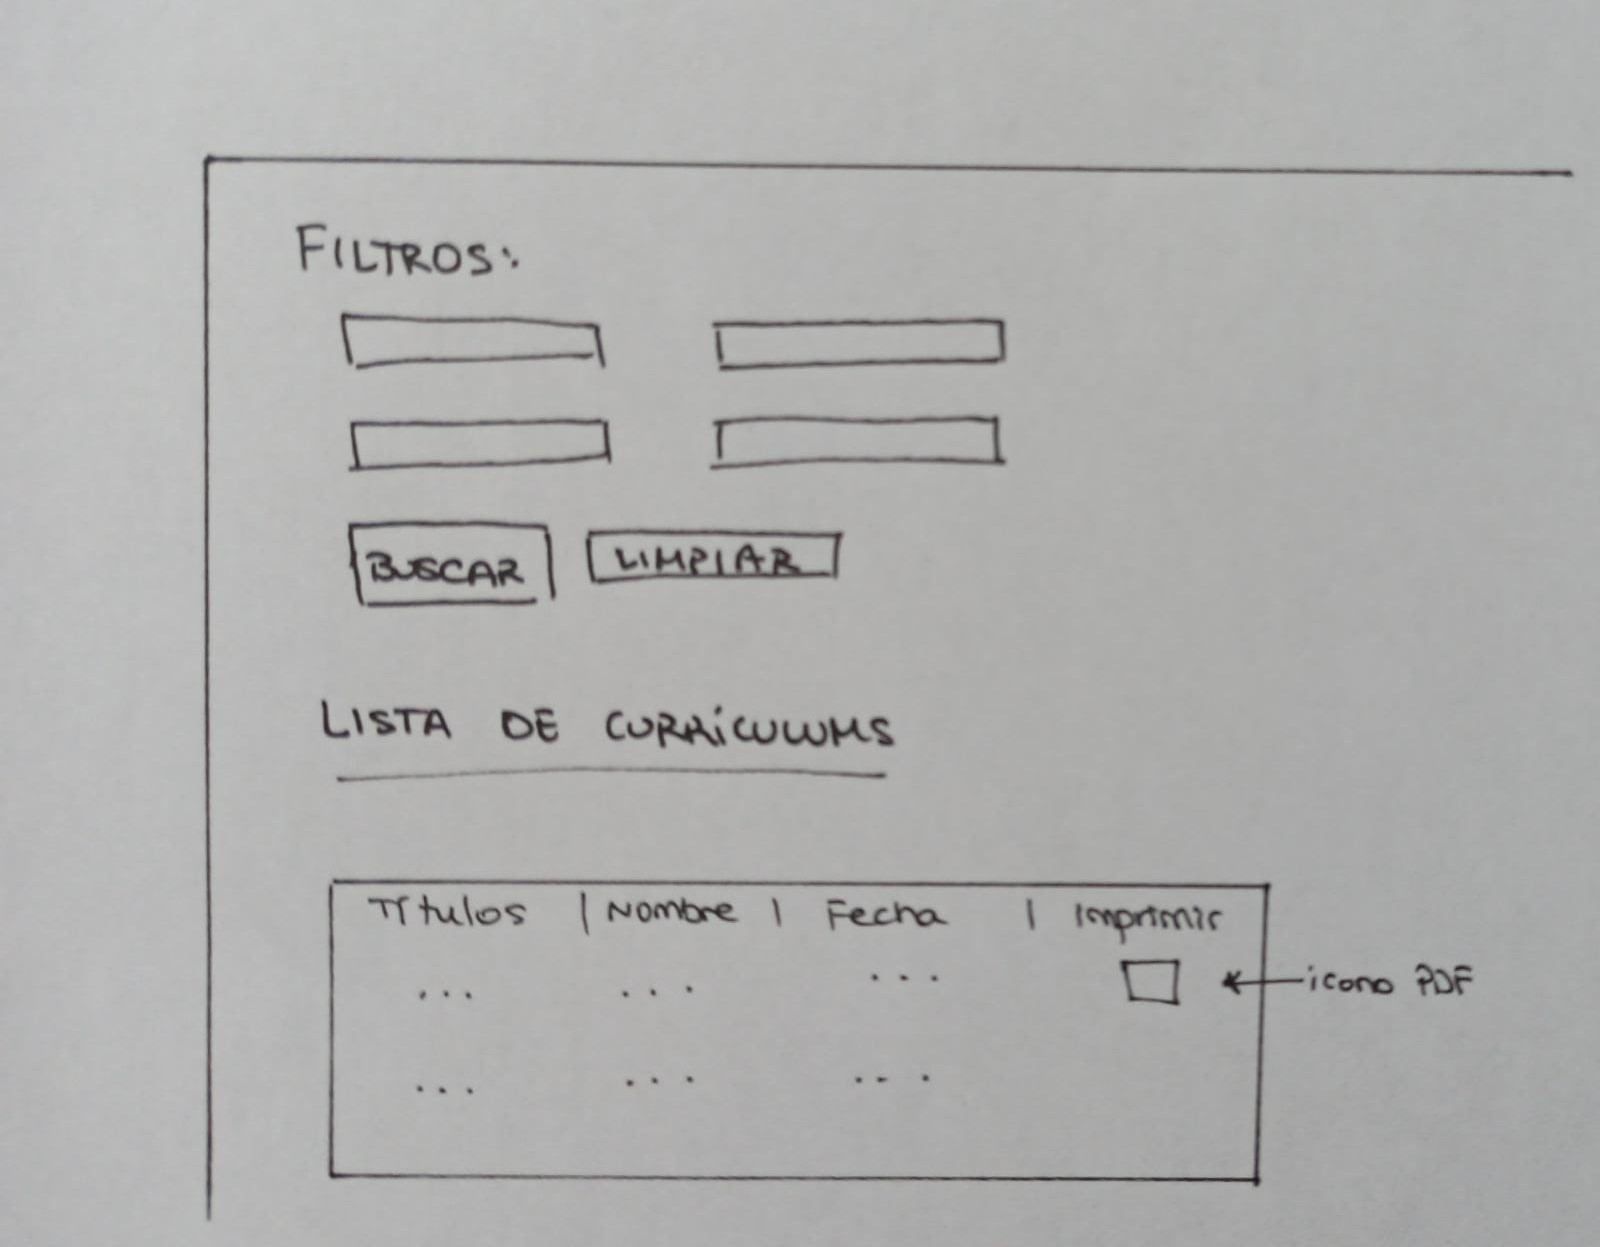
\includegraphics[width=\linewidth]{img/PT07-CVAdmin.jpeg}
    \caption{Prototipo 07. Vista de la administración de currículums}    
\end{figure}

\begin{figure}
    \centering
    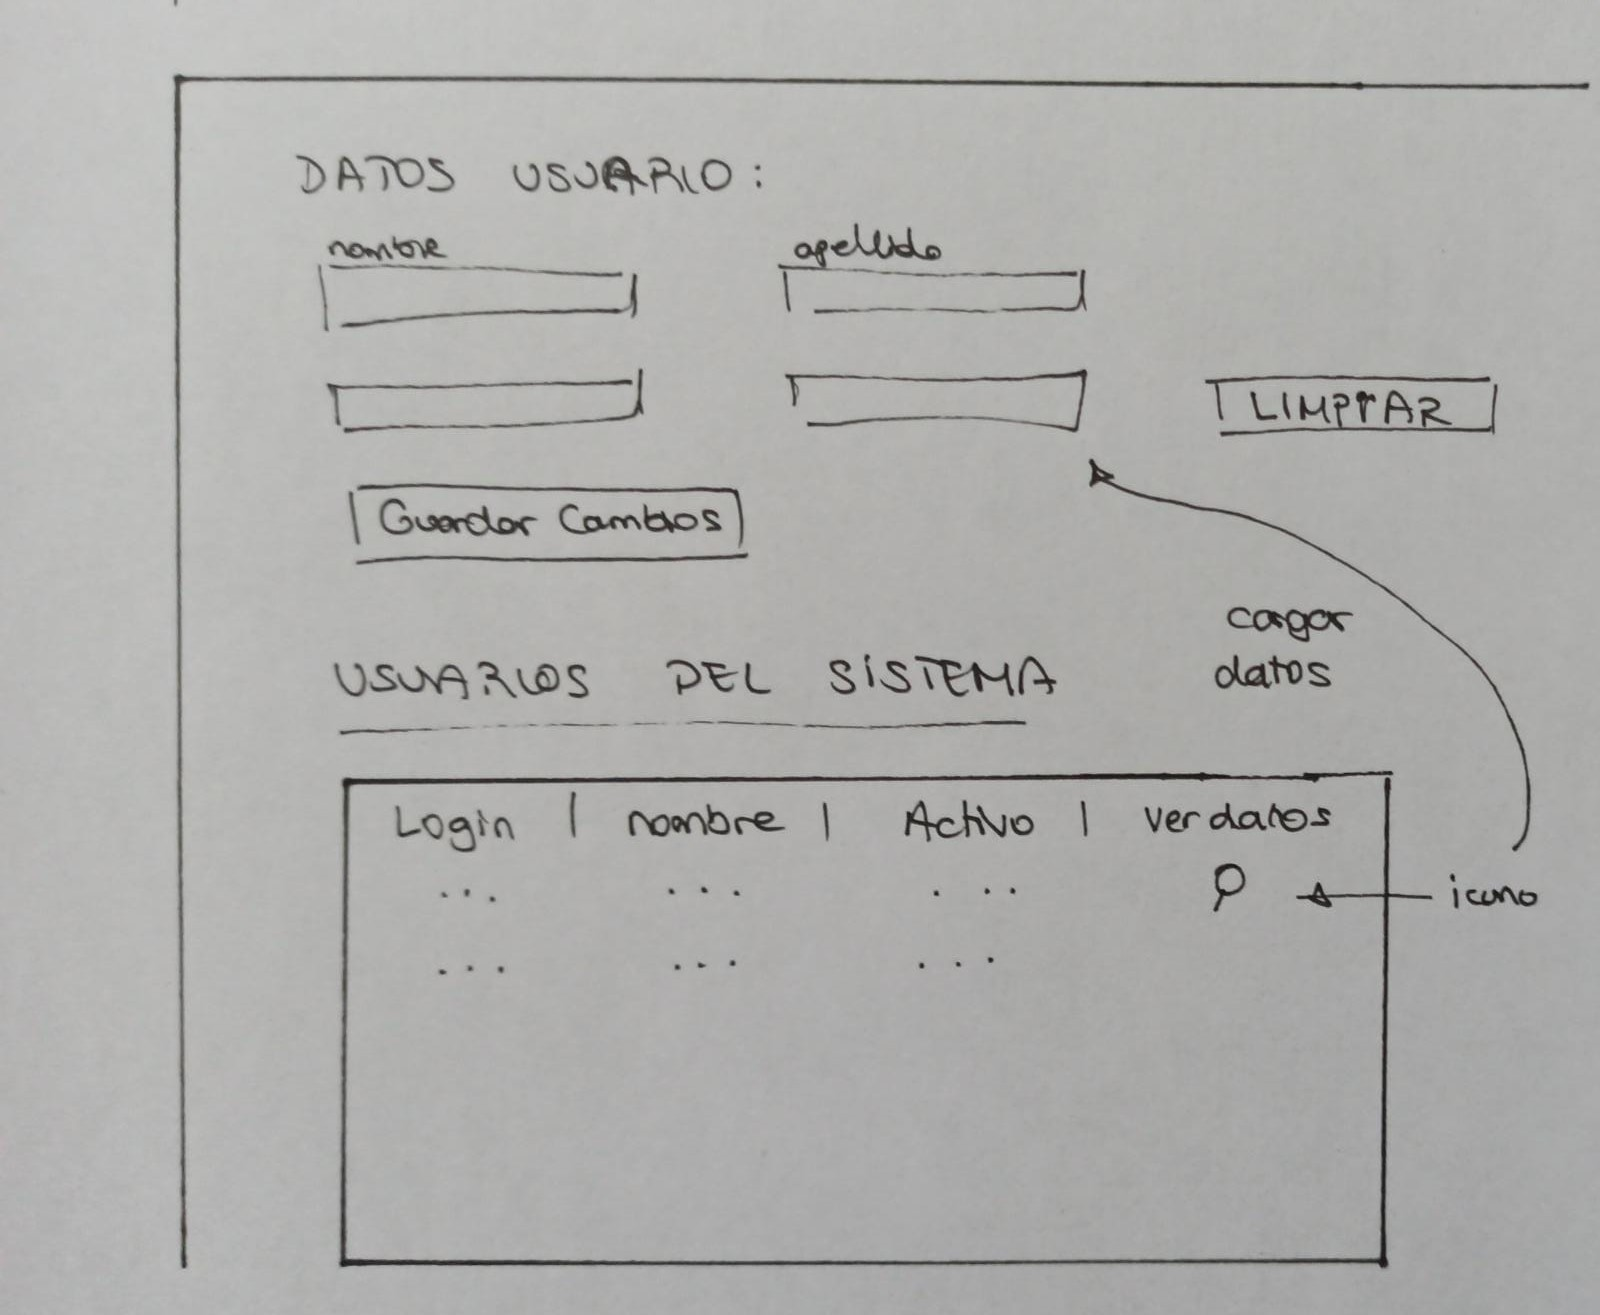
\includegraphics[width=\linewidth]{img/PT08-UserAdmin.jpeg}
    \caption{Prototipo 08. Vista de la administración de usuarios} 
\end{figure}




\apendice{Documentación técnica de programación}

\section{Introducción}
En este apartado se especificará la estructura de directorios de la aplicación y la instalación de materiales y recursos como una herramienta para programadores.

Para ello, se separará en tres secciones:
\begin{itemize}
    \item Estructura del repositorio: estructura de carpetas en git de la aplicación.
    \item Instalación, compilación y requisitos de entorno: explica cómo instalar y arrancar la aplicación y los requisitos para ello.
    \item Servicio web: se explicará la importación del despliegue a través de una máquina virtual para su posterior uso, así como la configuración de las instancias del servidor.
\end{itemize}

\section{Estructura del repositorio}
El repositorio en Git cuenta con la siguiente distribución principal:
\begin{itemize}
    \item \textbf{Directorios}: carpetas contenedoras de los archivos del proyecto.
    \item \textbf{Ramas o ``branches''}: distintas versiones del código de la aplicación en las distintas fases.
    \item \textbf{Issues}: tareas asignadas del proyecto.
    \item \textbf{Milestones}: hilo de proyecto que distribuye las tareas o issues. Cada milestone representa una fase o subfase del proyecto, que coincide con las etapas del modelo de la metodología usada y explicada previamente.
\end{itemize}

\subsection{Directorios}
Esta parte representa el contenido del proyecto en su totalidad. Las diferentes carpetas que se incluyen en el proyecto son:
\begin{itemize}
    \item \textbf{CSACVM}: es el núcleo y carpeta contenedora principal del proyecto. La estructura de esta carpeta se ha explicado previamente en el apartado de diseño, ya que es la que forma la aplicación con el resto de dependencias, librerías y subproyectos.
    \item \textbf{Documentación}: en esta carpeta se guarda toda la documentación del proyecto, como por ejemplo la memoria, los anexos, las imágenes utilizadas, etc.
    \item \textbf{DespliegueWeb}: carpeta contenedora de los archivos para la instalación del despliegue de la web con la máquina virtual.
    \item \textbf{ScriptsDB}: en esta carpeta se guardan los scripts de los datos de la base de datos que se utiliza por si se quiere instalar de forma local.
\end{itemize}

\subsection{Ramas, issues y milestones}
Las issues son las tareas asignadas del proyecto con las que se controlan los cambios de funcionalidad de este, tanto en código como a la hora de añadir/generar archivos, carpetas, estructura de proyecto o librerías.

Todas las issues tienen asignadas una milestone, ya que esta es la forma óptima de separar funcionalidad a través de las distintas fases del proyecto. Además de esto, las issues tienen labels que se han ido añadiendo y quitando durante su desarrollo.

Las labels más utilizadas han sido:
\begin{itemize}
\tightlist
    \item En proceso: issues que se encuentran en desarrollo en ese momento.
    \item \emph{Bug}: issues con partes que tienen errores que se intentan corregir.
    \item Documentation: issues para añadir o modificar los archivos de la documentación del proyecto.
    \item \emph{WontFix}: issues que se habían creado para cierto propósito que no se van a corregir o descartes de funcionalidad.
\end{itemize}

Como se ha explicado, las milestones forman cada distinta fase o etapa del flujo del desarrollo del proyecto. Cada milestone tiene:
\begin{itemize}
\tightlist
    \item Issues asignadas con la funcionalidad de esa etapa.
    \item Descripción de la fase y de las tareas que se llevarán a cabo.
\end{itemize}

Las milestones y las ramas también guardan relación, pues estas últimas guardan la versión del código en cada fase. Como diferencia, las milestones a veces dividen una rama o fase en varios subapartados.

Para dar un ejemplo del caso anterior, podemos tener una milestone de la fase 3 con varios subapartados (3.1, 3.2, 3.x...) pero todo se realiza en solamente una rama (rama para la fase 3).

\section{Instalación, compilación y ejecución del proyecto}
En esta parte del manual de programador, se va a explicar cómo realizar la instalación del proyecto y los requisitos para ello.

\subsection{Requisitos}
En primer lugar, necesitamos saber en qué entorno se va a utilizar el proyecto para saber qué herramientas debemos obtener antes de la clonación del proyecto. Para ello, necesitaremos:
\begin{itemize}
    \item \textbf{Entorno (IDE)}: el entorno que se utiliza es Visual Studio 2022, en mi caso personal se utiliza la versión ``Community'' (es gratuito) aunque tanto las versiones de ``Enterprise'' como ``Professional'' (ambas de pago con licencia) son igual de válidas 
    (a gusto del usuario).
    \item \textbf{SSMS}: Sql Management Studio 18 es el gestor de bases de datos que se utilizado para la realización del proyecto.
    \item \textbf{Git}: git es el controlador de versiones y a parte es una herramienta que permite ejecutar funciones para git. No es extremadamente necesario porque la clonación se hará a través de Visual Studio, pero también se explicará su uso a través de la consola de comandos.
\end{itemize}

Para la instalación de Visual Studio, se tienen que instalar ciertos paquetes:
\begin{itemize}
\tightlist
    \item Desarrollo de ASP.NET y web.
    \item Desarrollo de escritorio de \emph{.NET}.
    \item Desarrollo de \emph{Node.js}.
    \item Herramientas de \emph{EntityFramework} 6 y \emph{.NET WebAssembly}.
    \item SQL Server Express 2019 LocalDB.
    \item Paquetes de compatibilidad de \emph{.NET Framework} (del 4.6 al 4.8).
    \item ASP.NET MVC 4.
\end{itemize}

\subsection{Instalación}
Una vez tengamos las herramientas anteriores en nuestro sistema, daremos paso a la clonación del proyecto, importación de la base de datos y ciertos apuntes para la compilación que pueden servir a modo de ayuda.

\subsubsection{Clonación del repositorio con Visual Studio}
Es posible que nada más arrancar Visual Studio nos muestre una ventana para crear un nuevo proyecto o clonar uno existente.

\begin{figure}
    \centering
    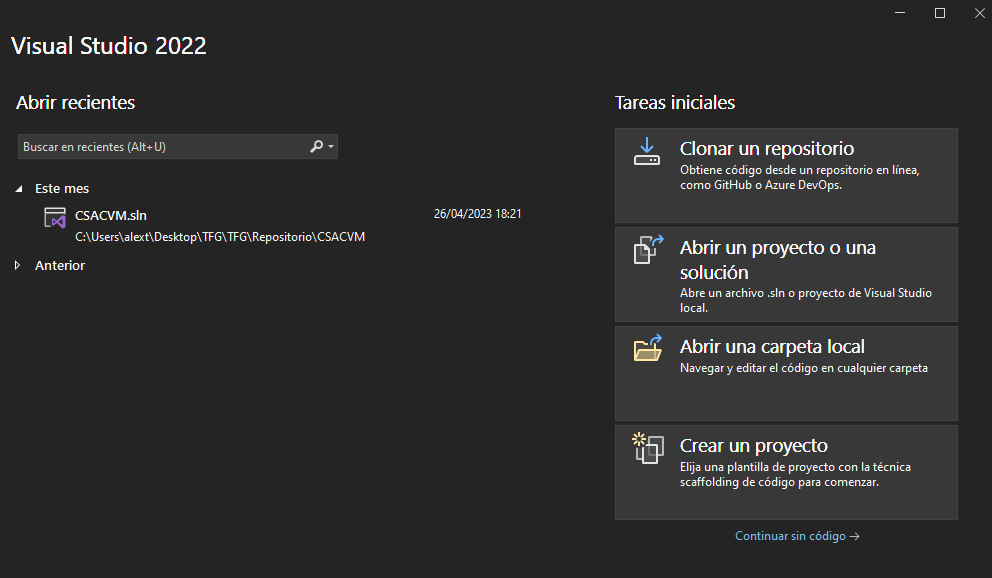
\includegraphics[width=\linewidth]{img/ManualProgramador/ClonacionP1.png}
    \caption{Clonación repositorio paso 1}
    
\end{figure}

Para clonar el repositorio, simplemente necesitamos copiar la url del repositorio en Github y especificar la carpeta donde va a estar nuestro proyecto en el sistema.

\begin{figure}
    \centering
    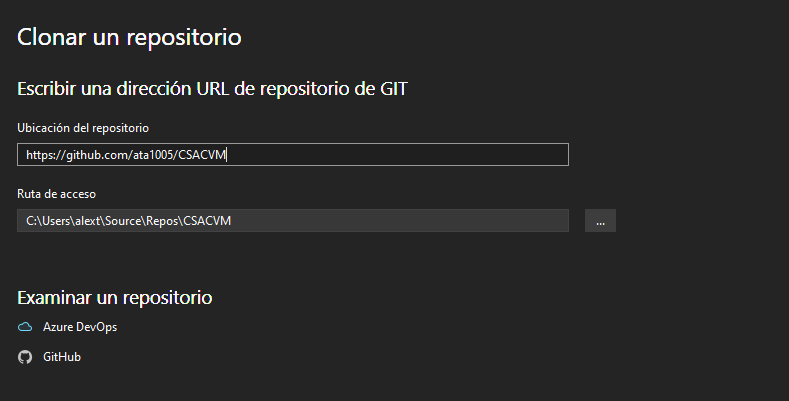
\includegraphics[width=\linewidth]{img/ManualProgramador/ClonacionP2.png}
    \caption{Clonación repositorio paso 2.1}
    
\end{figure}

También podemos añadir nuestra cuenta de Github y seleccionar el repositorio de forma manual.

\begin{figure}
    \centering
    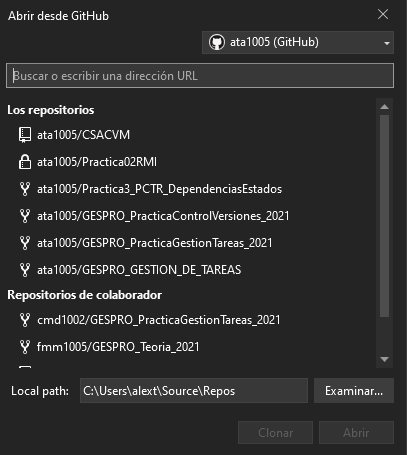
\includegraphics[width=\linewidth]{img/ManualProgramador/ClonacionP3.png}
    \caption{Clonación repositorio paso 2.2}
    
\end{figure}

\subsubsection{Clonación del repositorio con Git}
Para clonar el repositorio también podemos utilizar la consola de comandos de Git. En esta caso seguiremos los siguientes pasos:
\begin{itemize}
    \item Creamos una carpeta o directorio donde guardar el proyecto.
    \item Dentro de esa carpeta, abrimos la consola de Git (o en cualquier otro lado pero accediendo después a esta carpeta).
    \item Una vez dentro de la consola, escribimos el comando ``git clone'' seguido de la url que hemos copiado del repositorio del proyecto en github.
\end{itemize}

Una vez hecho esto ya solo queda entrar en Visual Studio y seleccionar nuestro proyecto entrando en la solución de la carpeta que hemos elegido.

\subsubsection{Añadir base de datos}
Como se ha indicado, los scripts para añadir la base de datos se encuentran en el repositorio de github. Una vez se haya instalado el SQL Management Studio, lo abrimos y seleccionamos el entorno o conexión en la que queremos conectarnos.

Por defecto se selecciona el ``localDB'' que es el host local del servidor de nuestro sistema, que se conecta a través de dos perfiles, dependiendo del sistema:
\begin{itemize}
\tightlist
    \item La cadena de conexión es solamente un punto (``.'').
    \item La cadena de conexión es: ``(localdb)\textbackslash MSSQLLocalDB''.
\end{itemize}

De todas maneras, si tenemos otro servidor en nuestro SQL en el que queramos añadir la base de datos, también lo podemos hacer.

Ahora solo nos queda importar la base de datos. Para ello, abrimos con el SQL Management Studio el script descargado y lo ejecutamos. Como el script que se incluye ya genera tanto la base de datos como las tablas y sus datos, no tendremos que hacer nada más.

\subsubsection{Configuración y compilación}
Si el servidor de base de datos fuera distinto al LocalDB, tendríamos que cambiar la cadena de conexión. Para ello debemos acceder al ``appsettings.json'' del proyecto principal, y cambiar el atributo de ``ConnectionStrings'', añadiendo en esa línea el enlace al servidor en el que se ha instalado la base de datos.

\begin{figure}[h]
    \centering
    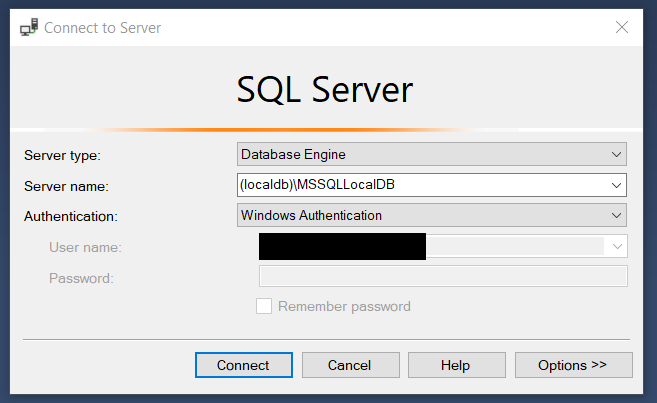
\includegraphics[width=\linewidth]{img/ManualProgramador/SQLConnect.png}
    \caption{Conexión en el SQL Management Studio}
\end{figure}
\begin{figure}
    \centering
    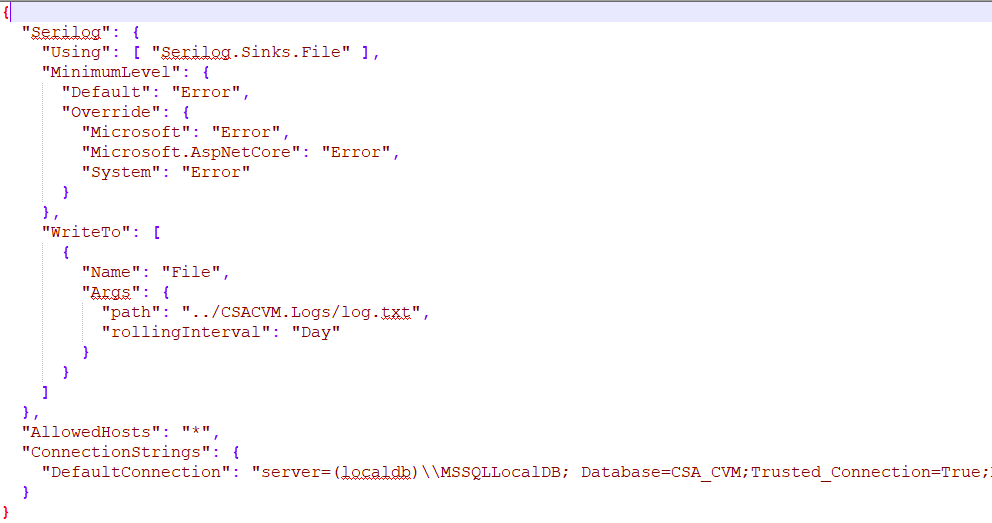
\includegraphics[width=\linewidth]{img/ManualProgramador/Settings.png}
    \caption{Cadena de conexión Programa - SQL Server}
    
\end{figure}

\newpage
Para compilar y ejecutar la aplicación, tenemos la configuración inicial. No obstante, podemos cambiar tanto el inicializador como el navegador que queramos utilizar.
\begin{figure}
    \centering
    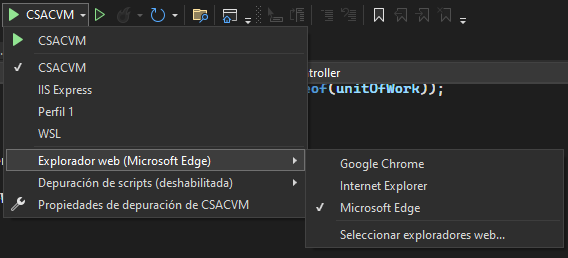
\includegraphics[width=\linewidth]{img/ManualProgramador/depuracion.png}
    \caption{Compilación y ejecución de la aplicación}
    
\end{figure}

\newpage
\section{Servicio web con máquina virtual}
Como se ha mencionado previamente, el despliegue del servidor web se realiza a través de una
máquina virtual de Windows 10.

Dentro de la máquina tenemos varias partes:
\begin{itemize}
\tightlist
    \item SQL Server: se instancia un servidor de base de datos en el que se aloja la database.
    \item IIS Express: configurador de los servicios web. En él se crea una instancia del proyecto, en el que se indica a qué directorio se apunta para obtener la configuración de la aplicación y lanzarla.
    \item Directorio web: en él guardamos los archivos de la publicación del proyecto.
\end{itemize}

\subsection{Configuración de los servicios}
Para crear la instancia de la web utilizaremos el IIS Manager.
\begin{figure}[H]
    \centering
    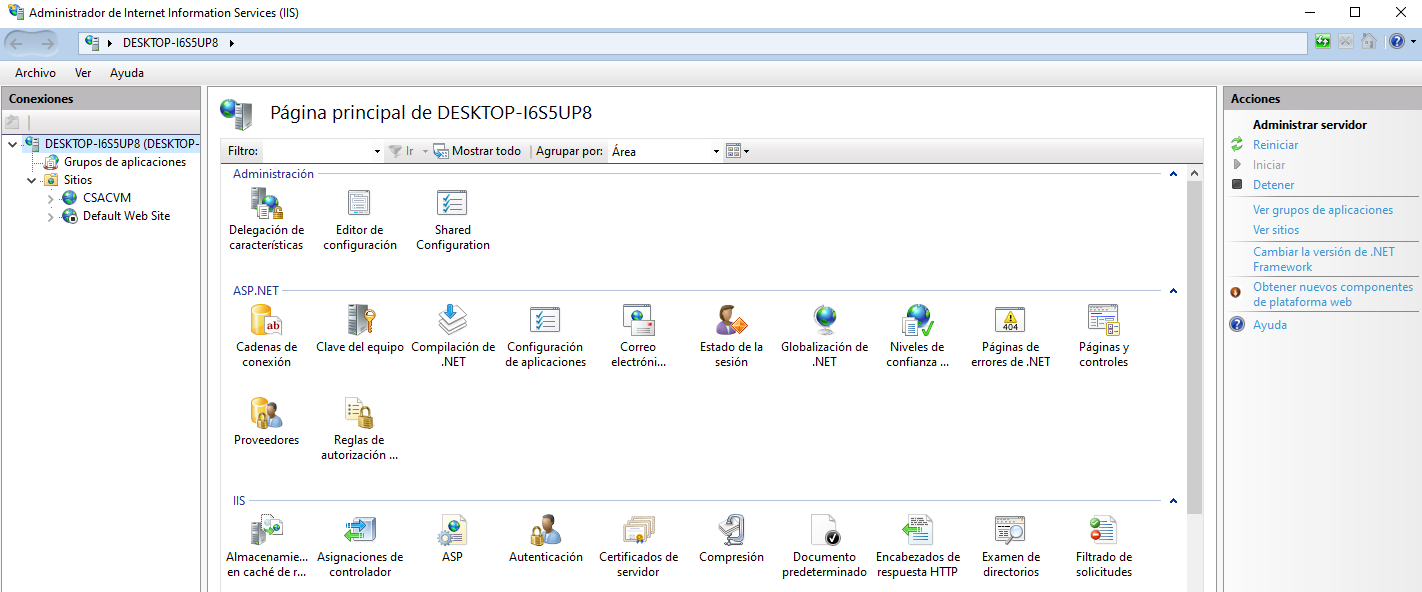
\includegraphics[width=\linewidth]{img/ManualProgramador/Despliegue01.png}
    \caption{IIS Manager - Página principal}
    
\end{figure}

Esta es la pantalla principal del configurador, en él se crean/instancian las aplicaciones web.
Como vemos en la parte de la izquierda, podemos configurar los grupos de aplicaciones y sus respectivos sitios web. 

\begin{figure}
    \centering
    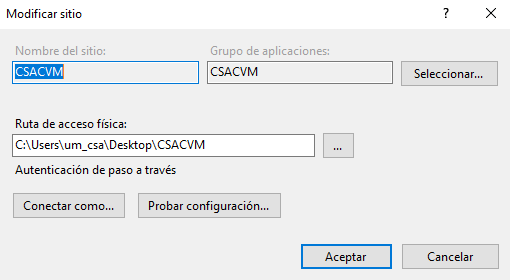
\includegraphics[width=\linewidth]{img/ManualProgramador/Despliegue02.png}
    \caption{IIS Manager - Configuración básica}
    \label{iisBasica}
\end{figure}

En la configuración básica (fig. \ref{iisBasica}), podemos indicar el nombre y la ruta de acceso directa al directorio donde se publica la aplicación, para que pueda obtener los archivos de configuración y desplegar la web.

\begin{figure}
    \centering
    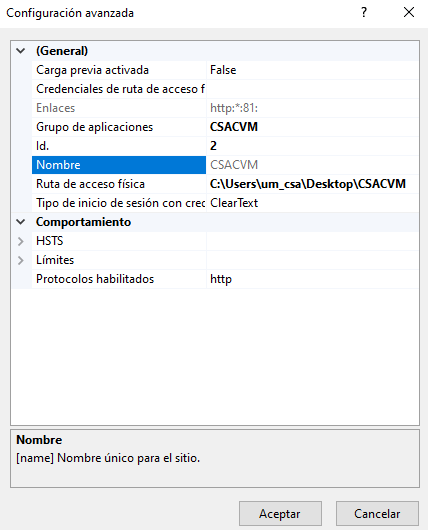
\includegraphics[width=\linewidth]{img/ManualProgramador/Despliegue03.png}
    \caption{IIS Manager - Configuración avanzada}
    \label{iisAvanzada}
\end{figure}

En la configuración avanzada (fig. \ref{iisAvanzada}) podemos indicar los hosts y los límites que vienen configurados. Normalmente estos atributos permanecen por defecto, pero se pueden personalizar. También es importante indicar el puerto en el que se despliega la web. Esto es importante porque el puerto es único para cada una de las páginas web que se van a alojar en el IIS.

Como la aplicación se ha desarrollado en Core, también ha hecho falta instalar un \href{https://learn.microsoft.com/en-us/aspnet/core/host-and-deploy/iis/hosting-bundle?view=aspnetcore-7.0}{``hosting bundle''}\footnote{Hosting Bundle para ASPNET Core: https://learn.microsoft.com/en-us/aspnet/core/host-and-deploy/iis/hosting-bundle?view=aspnetcore-7.0} que permite la ejecución de la web.

Finalmente, para la comunicación con la base de datos, se ha creado un usuario específico y se ha añadido directamente a la cadena de conexión de la aplicación, para que se pueda conectar con usuario y contraseña al servidor de base de datos.
\apendice{Documentación}

\section{Introducción}
En esta parte de la documentación se encuentra el manual de usuario, que será de utilidad para
el uso de la aplicación por parte de cualquier usuario. En él se enseña tanto a entrar en la aplicación a través de la máquina virtual, como de usar la aplicación en su totalidad.

\section{Manual de usuario}

\subsection{Acceder a la web}
Para acceder a la web, se puede hacer de dos formas:
\begin{itemize}
    \tightlist
    \item Si estamos utilizando el entorno virtual, el acceso es a través de cualquier navegador, introduciendo la dirección ``http://localhost:81''.
    \item Si estamos utilizando y lanzando la aplicación desde Visual Studio, al compilar y ejecutar nos carga la web directamente en el navegador que esté configurado (este se puede modificar desde el lanzador de Visual Studio).
\end{itemize}

\subsection{Inicio de sesión}
Una vez ejecutamos la aplicación, la primera pantalla que veremos es la de iniciar sesión.

\begin{figure}
    \centering
    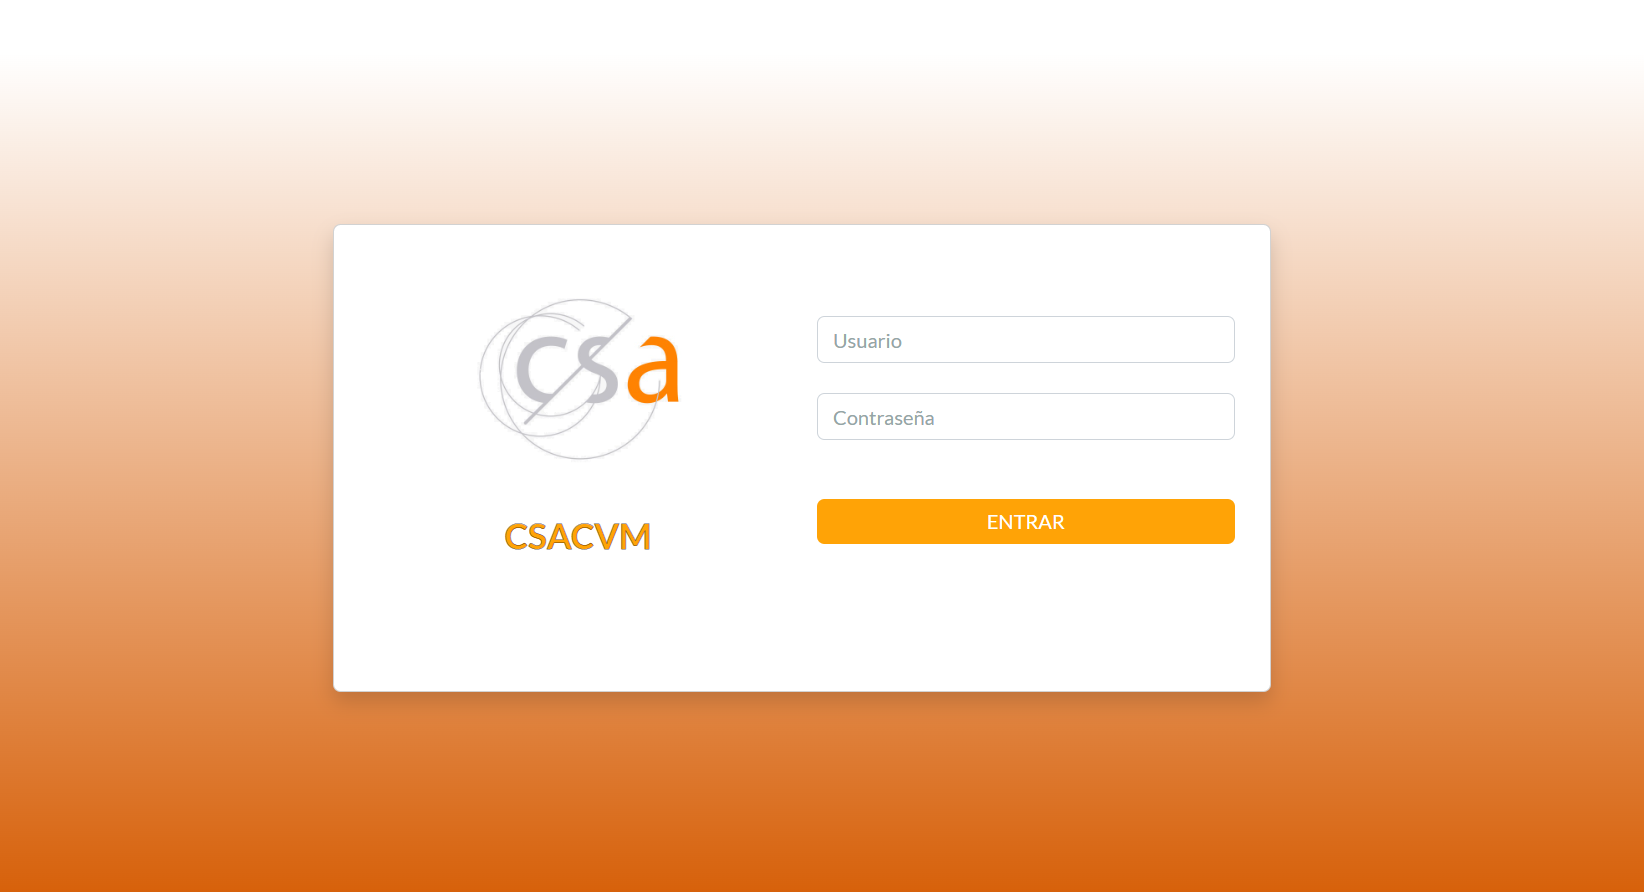
\includegraphics[width=\linewidth]{img/ManualUsuario/Manual01.png}
    \caption{Manual CSACVM - Inicio de sesión}
\end{figure}

Para entrar en la aplicación, debemos utilizar un usuario que esté registrado. Los usuarios se pueden crear a través de un administrador, pero actualmente, hay dos usuarios de prueba:
\begin{itemize}
    \tightlist
    \item Admin: admin.admin, contraseña = 1234.
    \item Usuario normal: userPrueba, contraseña = 2022.
\end{itemize}

Si la validación es correcta, se nos permitirá el acceso a la aplicación. 

\subsection{Página principal}
Una vez dentro de la aplicación, la pantalla principal tendrá el aspecto de la figura \ref{manualIndex}

\begin{figure}
    \centering
    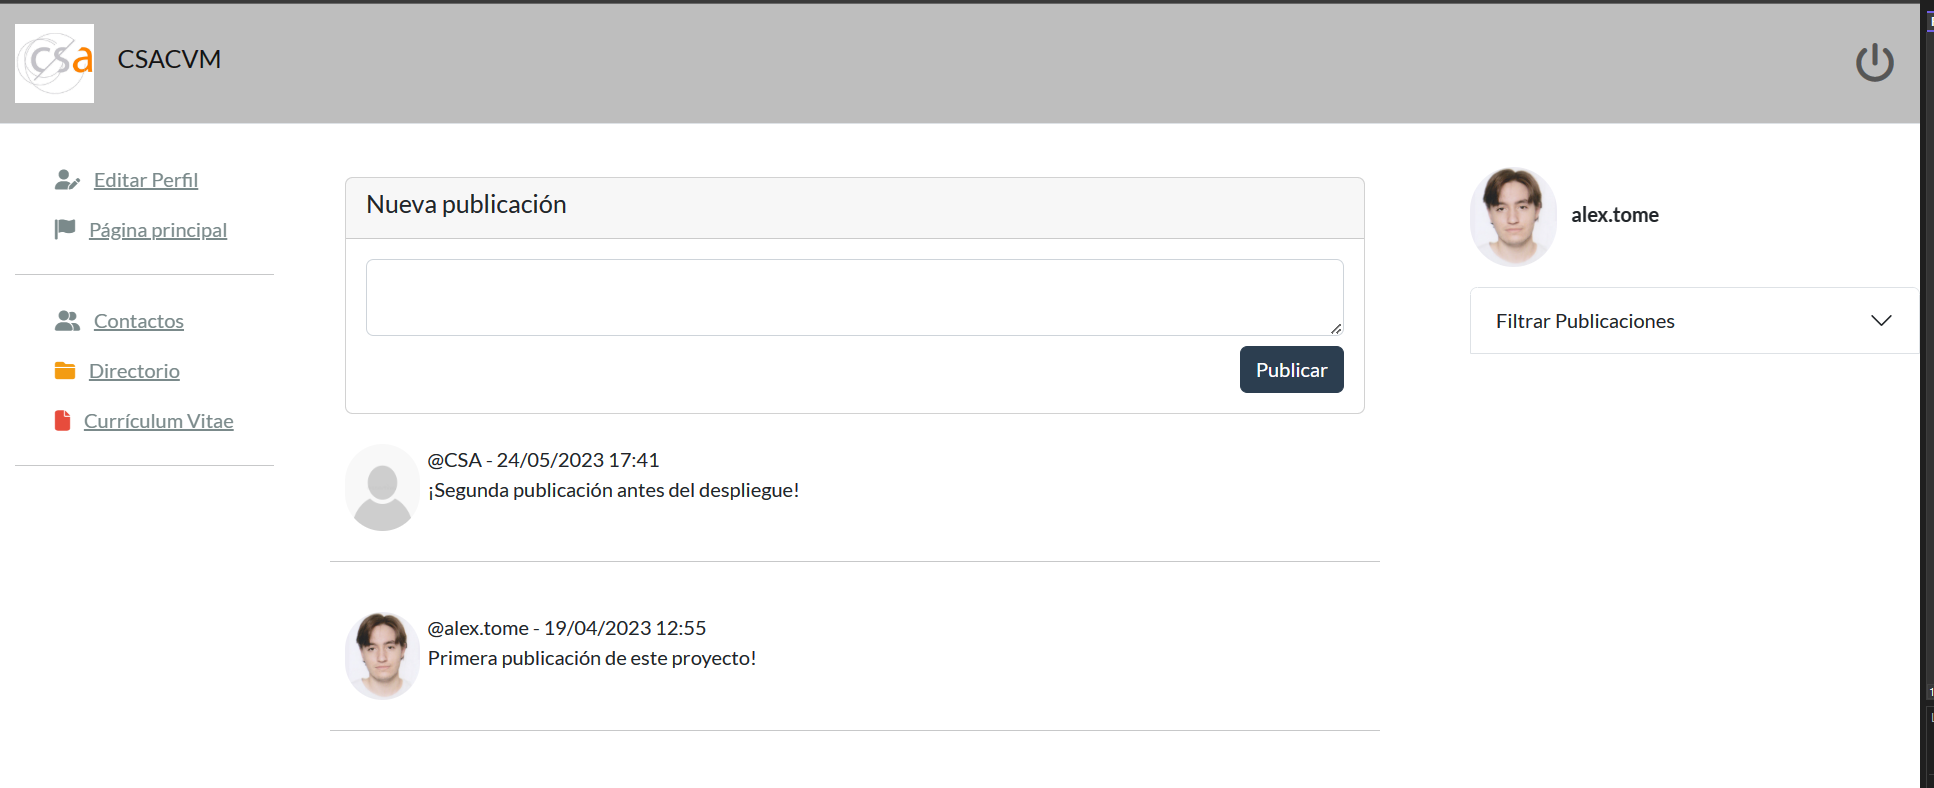
\includegraphics[width=\linewidth]{img/ManualUsuario/Manual02.png}
    \caption{Manual CSACVM - Layout y página principal} 
    \label{manualIndex}
\end{figure}

\begin{figure}
    \centering
    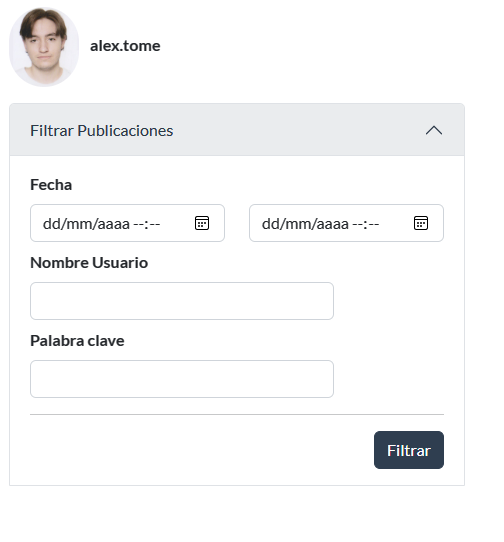
\includegraphics[width=.9\linewidth]{img/ManualUsuario/Manual03.png}
    \caption{Manual CSACVM - Filtros publicaciones} 
\end{figure}

En dicha pantalla podemos distinguir tres zonas distintas. A la izquierda, una barra con las distintas opciones para cada usuario, en el centro, las publicaciones de la aplicación y una zona para escribir un nuevo ``post'', y a la derecha, los filtros para la visualización de las publicaciones.

En los filtros de las publicaciones, podemos indicar el intervalo de fechas, el nombre de usuario o alguna palabra clave.

En el panel lateral izquierdo, las opciones dependerán del usuario con el que se haya iniciado sesión, tal y como se ve en la figura \ref{manualLayout}. 
\begin{figure}
    \centering
        \subfloat[Opciones no administrador]{
        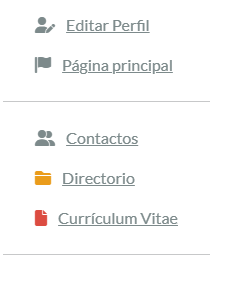
\includegraphics[width=0.4\textwidth]{img/ManualUsuario/Manual09.png}}
        \subfloat[Opciones administrador]{
        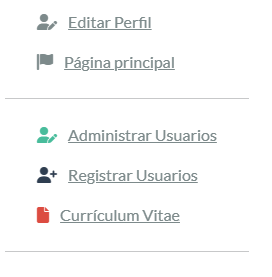
\includegraphics[width=0.4\textwidth]{img/ManualUsuario/Manual10.png}}
    \caption{Manual CSACVM - Panel lateral opciones}
    \label{manualLayout}
\end{figure}

Como vemos en la figura \ref{manualLayout}, dependiendo de si el usuario es administrador o no, nos saldrán unas opciones u otras, aunque haya varias que compartan ambos. Además, la vista de currículos también es distinta en cada caso.


\subsection{Perfil de usuario}
Si le damos en editar perfil, se nos mostrará nuestro perfil de usuario.
\begin{figure}
    \centering
    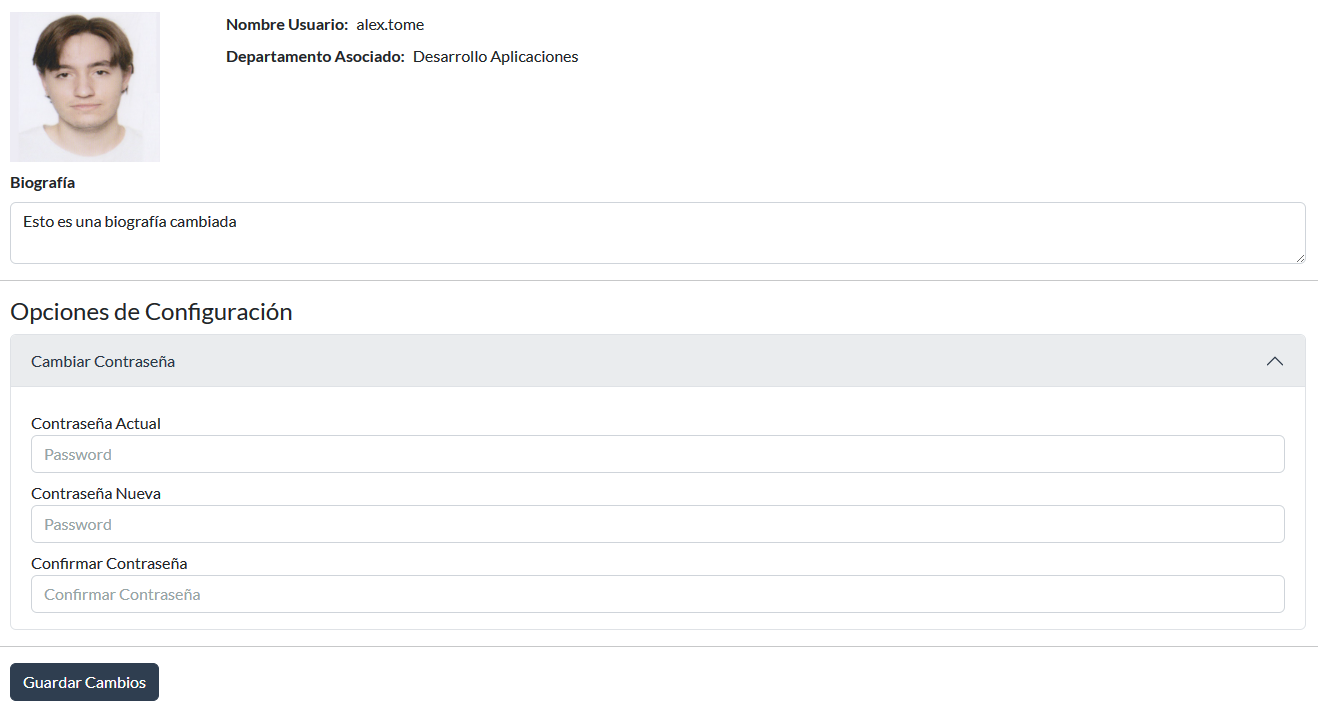
\includegraphics[width=\linewidth]{img/ManualUsuario/Manual04.png}
    \caption{Manual CSACVM - Perfil de usuario}
    \label{manualPerfil}
\end{figure}

En este apartado (fig. \ref{manualPerfil}), podremos hacer lo siguiente:
\begin{itemize}
    \item Cambiar la foto de perfil: al hacer click sobre la imagen, podemos subir una imagen desde nuestro directorio y cambiarla.
    \item Cambiar la biografía: al igual que cualquier red social, se permite añadir una biografía a modo de descripción del usuario.
    \item Cambiar contraseña: opción para cambiar la contraseña con la que entramos a la aplicación.
\end{itemize}

Para guardar los cambios, solo tenemos que pulsar al botón inferior.

\subsection{Contactos}
En el apartado de contactos, podemos buscar usuarios registrados en la aplicación y añadirlos como usuarios favoritos, similar a la funcionalidad que tiene skype.
\begin{figure}
    \centering
    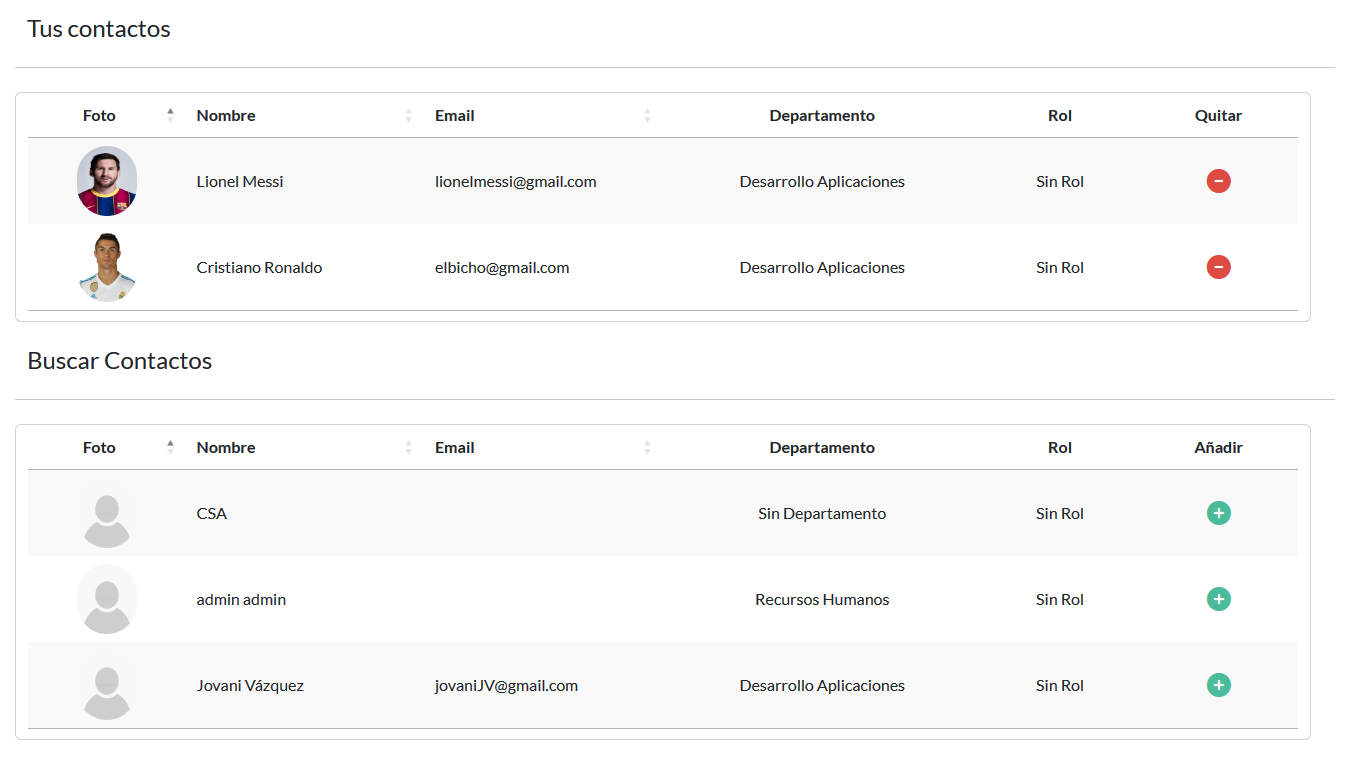
\includegraphics[width=\linewidth]{img/ManualUsuario/Manual05.png}
    \caption{Manual CSACVM - Contactos}
    
\end{figure}

De momento la funcionalidad es sencilla, en la tabla superior tenemos nuestros contactos, los cuales podemos quitar, y en la tabla inferior al revés.


\subsection{Directorio y notas}
En el directorio de usuario podemos crear notas. A través del botón superior, podemos darle título y contenido a una nota, la cual podremos ver, modificar o eliminar.
\begin{figure}
    \centering
    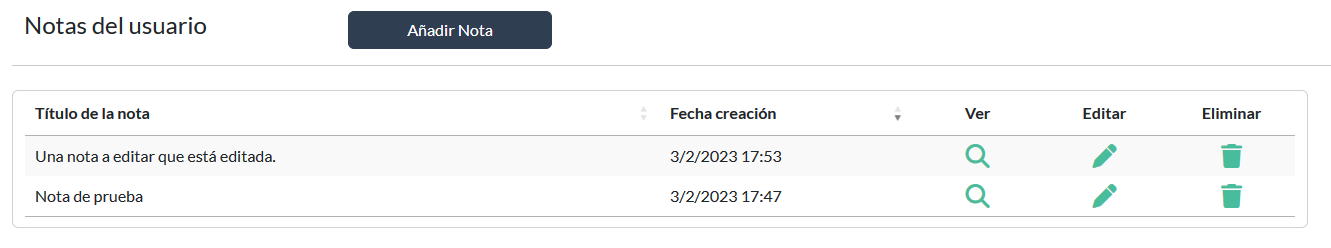
\includegraphics[width=\linewidth]{img/ManualUsuario/Manual06.png}
    \caption{Manual CSACVM - Directorio}  
\end{figure}

Para crear una nota, se nos abre la vista de la figura \ref{manualNotas}
\begin{figure}
    \centering
    \includegraphics[width=\linewidth]{img/ManualUsuario/Manual07.png}
    \caption{Manual CSACVM - Crear notas}
    \label{manualNotas}
\end{figure}

De esta forma podemos añadir un título que describirá el contexto de la nota y es lo que visualizaremos en la tabla, así como el contenido de la nota en sí.

\subsection{Currículum}
La vista de los currículos y la funcionalidad de cada uno de los apartados será distinta para cada tipo de usuario.
\subsubsection{Currículos para usuarios genéricos}
\begin{figure}
    \centering
    \includegraphics[width=\linewidth]{img/ManualUsuario/Manual11.png}
    \caption{Manual CSACVM - Currículos para no administradores}
    
\end{figure}

Esta es la vista para usuarios genéricos. La tabla contiene los currículos creados por el usuario que se encuentra en la aplicación. Para crear un nuevo currículum, solo tenemos que hacer click en el botón superior, e insertar el título del currículum.

También tenemos la opción de clonar a partir de otro currículum, de forma que se hará una copia de los datos de ese currículum a uno nuevo.

Una vez creado, tenemos las siguientes posibilidades:
\begin{itemize}
    \item \textbf{Editar}: es la funcionalidad principal, al hacer click en este botón, accederemos a una vista en la que tendremos las distintas opciones para rellenar el currículum.
    \item \textbf{Eliminar}: se hace un borrado completo del currículum.
    \item \textbf{PDF}: se hace una exportación del currículum a formato PDF.
\end{itemize}

Al hacer click en editar currículum, se nos mostrará la vista de la figura \ref{manualEditar}. Dentro de la vista tenemos varias etapas a rellenar:
\begin{figure}
    \centering
    \includegraphics[width=\linewidth]{img/ManualUsuario/Manual12.png}
    \caption{Manual CSACVM - Editar currículum}
    \label{manualEditar}
\end{figure}

\begin{itemize}
    \item \textbf{Información del usuario}: datos principales del usuario.
    \item \textbf{Formación Académica}: estudios del usuario.
    \item \textbf{Idiomas}: si se ha obtenido un título de un idioma.
    \item \textbf{Experiencia laboral}: los diferentes empleos que ha tenido el usuario.
    \item \textbf{Aptitudes y logros}: a modo de añadir información de carácter personal.
\end{itemize}


\begin{figure}
    \centering
    \includegraphics[width=\linewidth]{img/ManualUsuario/Manual13.png}
    \caption{Manual CSACVM - Editar currículum: formación académica}
    
\end{figure}

En este apartado podemos añadir tantas entradas como queramos, al igual que en los siguientes. 

En la formación podemos indicar el tipo de formación, qué estudios se han realizado, dónde y un campo de observaciones opcional de carácter informativo. 

Además de eso se indica cuándo se realizó.

\begin{figure}
    \centering
    \includegraphics[width=\linewidth]{img/ManualUsuario/Manual14.png}
    \caption{Manual CSACVM - Editar currículum: Idiomas} 
\end{figure}
En la parte de los idiomas, nos permite elegir el idioma, el nivel, la descripción o el título que se ha obtenido y dónde se realiza, además de indicar cuándo se realizó o se obtuvo el título.

\begin{figure}
    \centering
    \includegraphics[width=\linewidth]{img/ManualUsuario/Manual15.png}
    \caption{Manual CSACVM - Editar currículum: Experiencia laboral}
\end{figure}
En el apartado de la experiencia laboral se debe indicar el puesto principal de trabajo, la empresa en la que se realizó y su ubicación (esto último opcional), y un campo de observaciones para añadir más información sobre el puesto de trabajo, así como los años que se estuvo trabajando.

 
\begin{figure}
    \centering
    \includegraphics[width=\linewidth]{img/ManualUsuario/Manual16.png}
    \caption{Manual CSACVM - Editar currículum: Aptitudes y Logros} 
    \label{manualLogros}
\end{figure}
Finalmente tenemos los apartados de aptitudes y logros (fig. \ref{manualLogros}), que añaden información auxiliar para completar el currículum. Estos apartados son de carácter personal, en los que se indican atributos del trabajador como modelo de trabajo, personalidad, carácter, etc.

\subsubsection{Exportación a PDF}
\begin{figure}
    \centering
    \includegraphics[width=\linewidth]{img/ManualUsuario/Manual17.png}
    \caption{Manual CSACVM - Exportación PDF}
    \label{manualPDF}
\end{figure}
Los PDF's tienen el formato europeo de currículos (fig. \ref{manualPDF}), de modo que se encuentran, por un lado, la foto y los datos principales y más personales del usuario a la izquierda, y por otro, la experiencia laboral y la formación académica a la derecha (junto con el acerca de).

Al hacer un formato específico y estandarizado, todos los usuarios de la aplicación tendrán el mismo tipo de PDF y será más fácil para extraer datos y organizarlos por parte de la administración de la empresa.

\subsection{Currículum de administradores}
La vista de currículos para administradores es algo distinta (fig. \ref{manualCNA}). En primer lugar, los currículos que se ven en la tabla son todos los que están en el sistema de los diferentes usuarios.

\begin{figure}
    \centering
    \includegraphics[width=\linewidth]{img/ManualUsuario/Manual19.png}
    \caption{Manual CSACVM - Currículos para administradores}
    \label{manualCNA}
\end{figure}
En la parte superior tenemos los filtros, por los que podemos buscar los currículos en profundidad a través de los campos que queramos (idiomas, año nacimiento del usuario, nombre...). 

En la parte inferior tenemos la tabla con todos los currículos del sistema. Dentro podremos ver el contenido de los currículos o imprimirlos.

\begin{figure}
    \centering
    \includegraphics[width=\linewidth]{img/ManualUsuario/Manual20.png}
    \caption{Manual CSACVM - Ver currículum}  
\end{figure}

\subsection{Registro de usuarios}
\begin{figure}
    \centering
    \includegraphics[width=\linewidth]{img/ManualUsuario/Manual21.png}
    \caption{Manual CSACVM - Registro de usuarios}
    \label{manualRegistro}
\end{figure}
En la pantalla del registro de usuarios (fig. \ref{manualRegistro}), un administrador podrá añadir un usuario al sistema.
Para ello, debe completar los diferentes campos que se marcan. 

Hay varios de ellos que son obligatorios, como por ejemplo el nombre de usuario o la contraseña, que son con los que podrá entrar a la aplicación. Después tenemos campos opcionales como el email, el nombre y apellido, el departamento, el rol o el grupo.

Además de esto, podemos indicar si el usuario es administrador o no.

\subsection{Administración de usuarios}
\begin{figure}
    \centering
    \includegraphics[width=\linewidth]{img/ManualUsuario/Manual18.png}
    \caption{Manual CSACVM - Administración de usuarios}
    \label{manualAU}
\end{figure}

En la parte superior de la figura \ref{manualAU} tenemos los datos del usuario que elijamos a través del botón de ver de la tabla y podremos modificar sus campos. En la parte inferior tenemos la tabla con los usuarios del sistema y un sistema de filtros por los que buscar a los usuarios.








\nocite{*}
\bibliographystyle{plain}
\bibliography{bibliografiaAnexos}

\end{document}
